\documentclass[a4paper,11pt,twoside,openright]{book}							% COMANDI INIZIALI
\usepackage[italian]{babel}								% sillabazione italiana
\usepackage[utf8]{inputenc}								% Per le lettere accentate IN UNIX E IN WINDOWS
\usepackage{ragged2e}					 				% giustifica
\usepackage{amsmath}									% Per allineare le equazioni
\usepackage{amssymb}									% Per le lettere dell'indicatrice (mathbb)

\usepackage[sc]{mathpazo}
%Options: Sonny, Lenny, Glenn, Conny, Rejne, Bjarne, Bjornstrup
\usepackage[Sonny]{fncychap}
\usepackage{fancyhdr}
\pagestyle{fancy}
\fancyhead{} % cancella tutti i campi
\fancyfoot{}
\fancyhead[RE,LO]{\slshape \leftmark}
\fancyhead[LE,RO]{\thepage}
\renewcommand{\headrulewidth}{0.4pt}
%\renewcommand{\footrulewidth}{0.4pt}
\renewcommand{\chaptermark}[1]{%
\markboth{\thechapter.\ #1}{}}



\usepackage{graphicx}
\usepackage{amsthm}
\usepackage{amssymb}
\usepackage{amsmath}
\usepackage{mathtools}
\usepackage{caption}
\usepackage{booktabs}
\usepackage[linktocpage=true]{hyperref}
\usepackage{float}
\usepackage{subfigure}
\usepackage{multirow}
\usepackage{array}
\usepackage{lscape}	% Per la pagina di grafici
\usepackage[export]{adjustbox}
\usepackage{array,multirow,graphicx}
\usepackage[misc,geometry]{ifsym}


\DeclarePairedDelimiter{\abs}{\lvert}{\rvert}
\DeclarePairedDelimiter{\norma}{\lVert}{\rVert}
\DeclareMathOperator*{\argmin}{arg\,min}

\justifying 										% giustifica

\date{28 Luglio 2014}
\author{Gabriele Mazza}
\title{}

\begin{document}



\thispagestyle{empty}
\enlargethispage{60mm}
\begin{center}
\Huge{\textsc{Politecnico di Milano}}\\
\vspace{5mm}
\large{Scuola di Ingegneria Industriale e dell'Informazione}\\
\vspace{5mm}
\large{Corso di Studi in Ingegneria Matematica}\\
\vspace{10mm}
\begin{figure}[h]
	\begin{center}
	
\includegraphics[width=35mm]{Immagini/Logo.png}
	\end{center}
	\end{figure}
\vspace{5mm}
\large{Tesi di Laurea Magistrale}\\
\vspace{10mm}

\begin{LARGE}
TITOLO
\end{LARGE}
\vspace{30mm}

\begin{flushleft}
\begin{tabular}{l l }
Relatore:    & Prof. Laura SANGALLI \\
Correlatore: & Dott. Ing. Mara BERNARDI
\end{tabular}
\end{flushleft}
\vspace{12mm}
\begin{flushright}
\begin{tabular}{l l }
Tesi di Laurea di: & \\
Gabriele Mazza & Matr. 798794 \\
\end{tabular}
\end{flushright}
\vspace{12mm}
{\large{\bf Anno Accademico 2013-2014}}
\end{center}
\newpage
\thispagestyle{empty}

\chapter*{Sommario}
\label{Cap:sommario}
\thispagestyle{empty}
Il presente lavoro di tesi propone un modello separabile per l'analisi funzionale di dati distribuiti in spazio e tempo. Il modello è particolarmente adatto allo studio di problemi con domini spaziali complessi, con concavità o buchi. La capacità di tener conto della geometria spaziale rappresenta un forte vantaggio per questo modello, che sarà paragonato alle altre tecniche già esistenti, comprese quelle che non presentano tale particolarità. Oltre allo sviluppo analitico è stato creato un algoritmo e un codice R per il calcolo computazionale della stima. La principale applicazione studiata in questa tesi riguarda la produzione di rifiuti urbani pro capite nei comuni della provincia di Venezia tra il 1997 e il 2011, con un'attenzione speciale agli effetti legati al turismo.

\newpage
\thispagestyle{empty}
\chapter*{Abstract}
\label{Cap:abstract}
\thispagestyle{empty}
The present work of thesis proposes a separable model for the functional analysis of data distributed in space and time. The model is particularly appropriate to the study of problems with complex spatial domains, with concavities or holes. The ability to consider the spatial geometry is a strong advantage of this model, which will be compared to other existing techniques, including those that haven't this peculiarity. In addition to the analitical definition, an algorithm ad an R code for the computation of the estimate has been created. The main application studied in this thesis regards the production of urban waste per capita in the municipalities of Venice province between 1997 and 2011, with a special attention to the effects related to tourism.
\newpage
\thispagestyle{empty}

\chapter*{Ringraziamenti}
\thispagestyle{empty}
da fare
\newpage
\thispagestyle{empty}

%INIZIO DELLA NUMERAZIONE
\frontmatter
\tableofcontents
\markboth{Indice}{Indice}
\listoffigures
\markboth{Elenco delle figure}{Elenco delle figure}
\listoftables
\markboth{Elenco delle tabelle}{Elenco delle tabelle}
\newpage
\thispagestyle{empty}
\mainmatter

\chapter*{Introduzione}
\label{Cap:intro}
\addcontentsline{toc}{chapter}{Introduzione}
\markboth{Introduzione}{Introduzione}
\thispagestyle{empty}

Il presente lavoro di tesi si occupa della costruzione e dell'applicazione di un modello statistico per l'analisi funzionale di dati tempo-varianti e distribuiti su un dominio spaziale. Questa ricerca è motivata dalla necessità di avere un buon metodo d'analisi per i dati riguardanti la produzione dei rifiuti urbani pro capite nei comuni della provincia di Venezia. I dati sono stati raccolti ed elaborati dall'Agenzia Regionale per la Prevenzione e Protezione Ambientale del Veneto (Arpav) e sono disponibili sul sito di Open Data Veneto\footnote{\href{http://dati.veneto.it/dataset/produzione-annua-di-rifiuti-urbani-totale-e-pro-capite-1997-2011}{http://dati.veneto.it/dataset/produzione-annua-di-rifiuti-urbani-totale-e-pro-capite-1997-2011}}. Le misurazioni sono state registrate per comune. In fig. \ref{fig:intro} è stata tracciata la descrizione del dominio con i punti in cui i dati sono localizzati. Il problema presenta anche la dipendenza dal tempo, poiché i dati sono riportati annualmente dal 1997 al 2011.

\begin{figure}[h]
	\centering
	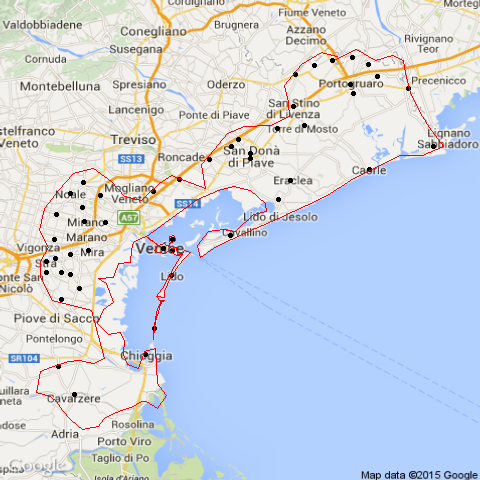
\includegraphics[width=0.46\textwidth]{Immagini/Ven_punti.png}   
   	\caption{Dominio spaziale e locazioni dei dati}
	\label{fig:intro}
\end{figure}
\newpage
\begin{figure}[t]
	\centering
	\subfigure[Rifiuti pro capite nel 2011]
   {
	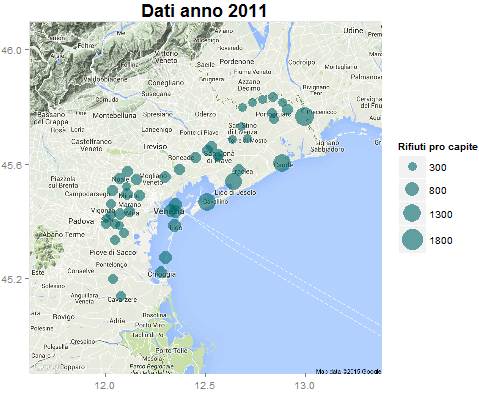
\includegraphics[width=0.46\textwidth]{Immagini/venezia_dati/Dati2011.png}   
   }
	\subfigure[Posti letto pro capite nel 2011]
   {
	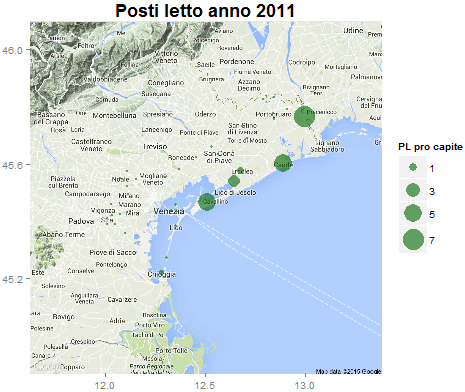
\includegraphics[width=0.46\textwidth]{Immagini/venezia_dati/PL2011.png}
   }
	\caption{Rifiuti e posti letto pro capite}
	\label{fig:intro2}
\end{figure}
La produzione di rifiuti urbani sarà certamente influenzata anche dal turismo. Per questo motivo sarà considerato nel modello anche questo effetto, non trascurabile nella stima, attraverso il numero di posti letto pro capite nei comuni (maggiori dettagli saranno forniti in seguito). In fig. \ref{fig:intro2} sono visualizzati i valori dei rifiuti e dei posti letto pro capite nel 2011, anno più recente nel dataset, come esempio di ciò che si ha a disposizione.

Il problema della produzione dei rifiuti nella provincia di Venezia richiede la formulazione di un modello per l'analisi funzionale di dati definiti in spazio e tempo particolarmente adatto. Sono già disponibili in letteratura tecniche per dati di questo tipo ma non tutte sono adatte al trattamento di questi dati. La geometria del dominio, infatti, è complessa. In alcuni punti essa ha una definizione per nulla grossolana e presenta una grossa concavità nella laguna di Venezia, oltre alle numerose isole. Pertanto non si può evitare di considerare le particolarità del dominio spaziale.

Si consideri ad esempio quanto riportato in \ref{fig:intro3}. Sono stati riportati i comuni di Quarto d'Altino e Cavallino-Treporti, tra di loro non eccessivamente distanti in linea d'aria ma con valori di produzione dei rifiuti decisamente diversi (come si può notare dagli andamenti temporali). Se i dati fossero analizzati con una tecnica che non tiene conto della geometria spaziale i due comuni sarebbero ritenuti vicini tra loro, quando in realtà si ha una grande separazione dovuta alla laguna di Venezia. Tecniche che trascurano la forma del dominio non sono appropriate poiché porterebbero ad una cattiva stima del fenomeno.
\newpage
\begin{figure}[t]
	\centering
	\subfigure[Comuni selezionati]
   {
	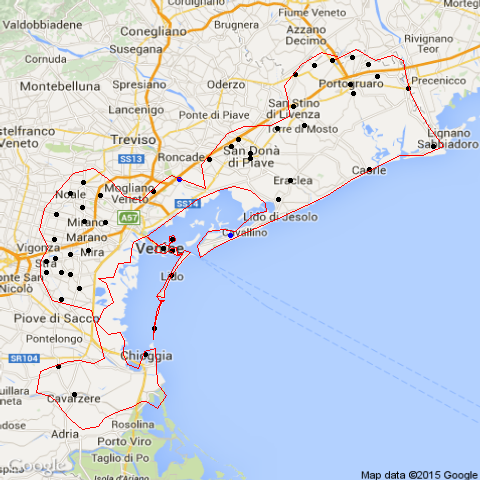
\includegraphics[width=0.43\textwidth]{Immagini/CTQDA.png}   
   }
	\subfigure[Andamenti temporali]
   {
	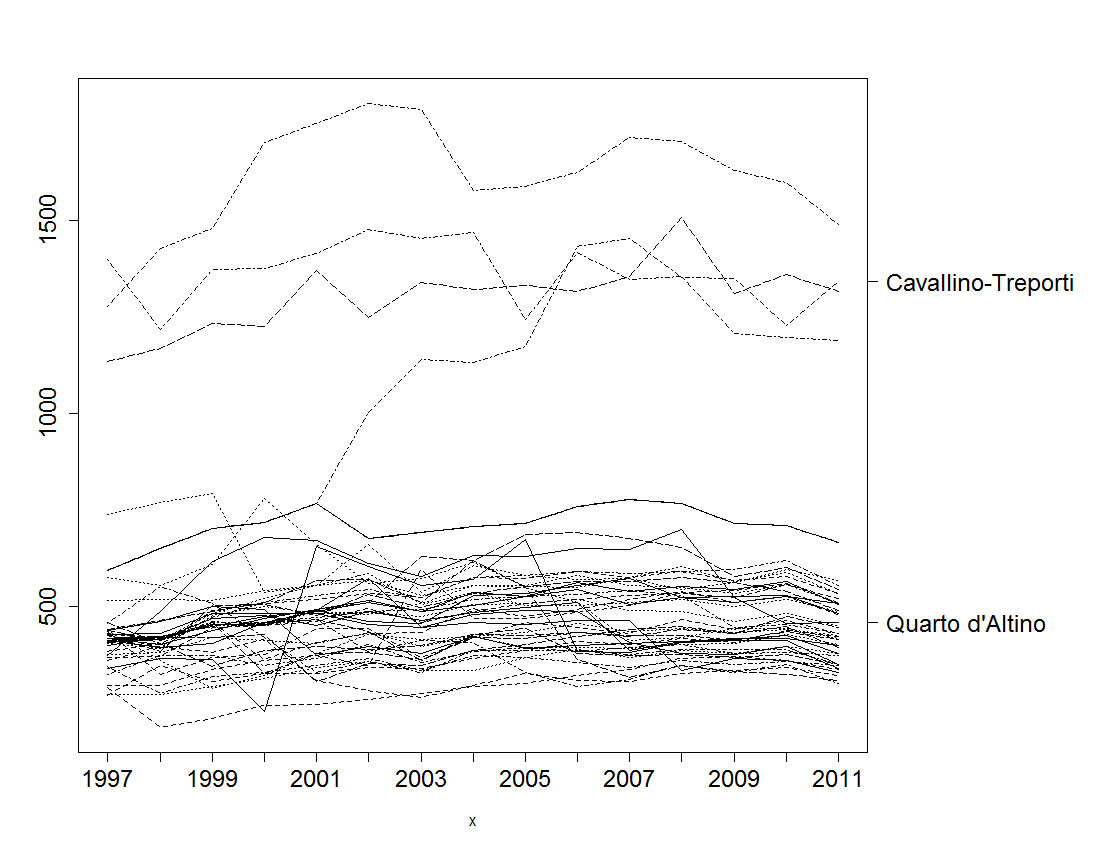
\includegraphics[width=0.49\textwidth]{Immagini/andamenti_temporali.png}
   }
	\caption{Differenza tra i dati nei comuni di Cavallino-Treporti e Quarto d'Altino}
	\label{fig:intro3}
\end{figure}
In questa tesi sarà illustrato il modello statistico \textit{Spatio-Temporal Regression model with PDE penalization} (ST-PDE) per l'analisi funzionale di dati distribuiti in spazio e tempo. Questo modello si dimostrerà in grado di assolvere pienamente questo compito e di fornire una buona stima dell'andamento della produzione di rifiuti urbani nella provincia di Venezia. La funzione sarà stimata dalla minimizzazione di un funzionale di penalizzazione con termini differenziali, quindi sarà garantita anche la regolarità della stima. La funzione stimata sarà espressa secondo opportune funzioni di base (elementi finiti in spazio, B-splines in tempo) capaci di tener conto della geometria spaziale. Tramite l'aggiunta di un termine con covariata sarà possibile introdurre anche dell'effetto del turismo. Dalla modellizzazione matematica è stato sviluppato un algoritmo e il conseguente codice R per il calcolo della soluzione numerica della stima. 

Il lavoro di tesi sarà strutturato come segue. Nel capitolo \ref{cap:panoramica} è riportato una panoramica dei metodi già esistenti in letteratura. Nel capitolo \ref{cap:modello} è presentata la costruzione del modello matematico ST-PDE, seguita dallo sviluppo del codice R descritto nel capitolo \ref{cap:Codice}. Nel capitolo \ref{cap:domC} si hanno i primi risultati, derivanti dall'applicazione del modello e del codice R a simulazioni eseguite sul dominio a forma di C descritto in \cite{art:ramsay} e \cite{art:wood}, per il quale è possibile valutare la bontà delle stime ottenute grazie alla perfetta conoscenza del fenomeno reale in ogni punto e in ogni istante. Nel capitolo \ref{cap:confronto} il modello ST-PDE sarà paragonato ad altri metodi già esistenti per il confronto delle stime ottenute. Nel capitolo \ref{cap:rifiuti} si ha l'applicazione allo studio della produzione dei rifiuti nella provincia di Venezia e infine, nel capitolo \ref{cap:conclusione}, sono raccolte le conclusioni e i possibili sviluppi futuri.
\newpage
\thispagestyle{empty}

\chapter{Panoramica sui modelli già esistenti}
\label{cap:panoramica}

Il modello ST-PDE si inserisce nell'ambito dell'analisi funzionale di dati distribuiti in spazio e tempo. Sia $\underline p = (x,y) \in \Omega$ il vettore con le coordinate del punto spaziale, $t \in [T_1,T_2]$ l'istante temporale e $z \in \mathbb{R}$ la variabile risposta. Le metodologie classiche di analisi funzionale, esposte ad esempio in \cite{art:ramsaysilverman}, possono essere applicate per la stima di un dato tempo-variante. Tuttavia in questo caso si ha anche la dipendenza spaziale, pertanto la funzione da stimare sarà:
$$
z=f(\underline p,t) \ .
$$
Secondo quanto è solitamente fatto per problemi di analisi di dati funzionali, sarà necessario minimizzare un funzionale di penalizzazione che contenga non soltanto gli scarti tra valori osservati e stimati ma anche termini differenziali per la regolarità della stima.

La letteratura su modelli spazio-temporali è già ampia, come è esposto in \cite{art:cressie}. Tuttavia le metodologie già disponibili presentano tra loro delle differenze. Non tutti i modelli sono adatti ad essere applicati alla stima della produzione di rifiuti urbani nella provincia di Venezia a causa della forte dipendenza dalla geometria del problema. Per questo motivo, dopo la definizione del modello ST-PDE, sarà dedicato anche uno spazio al al confronto delle stime dai tra i diversi metodi a disposizione su dati appositamente generati.

Ad esempio, il kriging spazio-temporale, descritto in \cite{art:caballero}, \cite{art:menafoglio1} e \cite{art:menafoglio1}, non è in grado di tener conto del dominio spaziale. Questa tecnica sarà considerata negli studi di simulazione e nei confronti ma non potrà garantire risultati ottimali per questo tipo di analisi.

Le pubblicazioni \cite{art:augustin} e \cite{art:marra} studiano metodi per l'analisi funzionale di dati distribuiti in spazio e tempo. Questo lavori, però, si basano su modelli che possono assumere una forma più complessa, ipotizzando che una funzione del valore atteso della risposta (nel loro caso il logaritmo) possa essere spiegato da uno o più termini funzionali (quest'ultima possibilità è riportata solo in \cite{art:augustin}):
$$
\log(\mathbb{E}[z_i])= f_1+f_2+ \ldots f_N .
$$
Ognuna di queste funzioni può avere dipendenza solo spaziale, solo temporale o entrambe. Queste complicazioni rispetto al modello che sarà studiato da ST-PDE possono essere risolte molto velocemente ipotizzando che la risposta dipenda da un solo termine spazio-temporale. Le tecniche proposte dagli autori sono un ottimo termine di paragone per il modello ST-PDE. La loro applicabilità per un problema con forte dipendenza dalla forma del dominio, come sarà spiegato più nel dettaglio in \ref{cap:confronto}, dipende dalla scelta delle funzioni di base. 

Particolare attenzione deve essere posta riguardo a quanto fatto in \cite{art:sangalli}. In questa pubblicazione è studiato un modello solamente spaziale, definito su un dominio $\Omega$. Tale dominio può assumere le stesse caratteristiche che saranno studiate in questa tesi: definizione complessa, concavità o buchi. La risposta è espressa dal seguente modello:
$$
z=f(\underline{p})
$$
Per poter stimare la funzione $f$ è introdotto il seguente funzionale di penalizzazione da minimizzare:
$$
J_{\lambda }(f(\underline p))=\sum_{i=1}^n \bigl( z_{i} - f(\underline p_i) \bigr)^2 \ + \\
+\lambda\int_{\Omega} ( \Delta(  f(\underline p)  ) \Bigr)^2 d \Omega \ .
$$
Il problema di minimo è risolto attraverso il passaggio ad una forma variazionale che, a seguito dell'introduzione di un'opportuna espansione in elementi finiti per $f$, è ridotta ad un problema discreto risolvibile con un sistema lineare. L'articolo \cite{art:sangalli} non contempla la variazione temporale per $f$ ma può essere considerato il punto di partenza per il modello ST-PDE. Non sarà ricavata una forma variazionale per la stima della soluzione, ma l'attenzione alla geometria del problema e l'uso degli elementi finiti rappresentano un forte legame con il modello ST-PDE.

\chapter{Presentazione del modello ST-PDE}
\label{cap:modello}
In questo capitolo è descritto nel dettaglio il modello ST-PDE per l'analisi di dati distribuiti in spazio e tempo ed è calcolata la soluzione al problema di stima.


\section{Caso senza covariate}

\subsection{Dati e modello}

Sia $\{\underline p_i = (x_i,y_i); i=1, \ldots , n\}$ un insieme di $n$ punti spaziali in un dominio limitato $\Omega \subset \mathbb R^2$ e sia $\{t_j ; j=1, \ldots , m\}$ un insieme di $m$ istanti temporali in un intervallo $[T_1,T_2]\subset \mathbb R$. In questi punti ed istanti si osservano i dati: siano quindi $\{ z_{ij};i=1, \ldots , n; j=1, \ldots , m \}$ i valori della variabile risposta nel punto $\underline p_i$ al tempo $t_j$.

Come già riportato nel capitolo precedente, l'obiettivo sarà la stima di un campo spazio-temporale che rappresenti il fenomeno da cui sono stati raccolti i dati. Quindi si ipotizza che le osservazioni $z_{ij}$ siano generate da tale campo spazio-temporale con l'aggiunta di rumore:
\begin{equation}
\label{eq:modellobase}
z_{ij}=f(\underline p_i,t_j)+\varepsilon_{ij}\ \ \ \ i = 1,\ldots,n\ \ j=1,\ldots,m \ \ ,
\end{equation}
dove $\{ \varepsilon_{ij}; i = 1,\ldots ,n; j=1,\ldots m\}$ sono residui indipendenti identicamente distribuiti di media nulla e varianza $\sigma^2$. L'obiettivo del modello ST-PDE sarà la stima della funzione $f(\underline p,t)$ dalle $nm$ osservazioni a disposizione, minimizzando un funzionale $J_{\underline \lambda }(f(\underline p,t))$ con la somma degli scarti quadratici tra le osservazioni e valori stimati e termini di penalizzazione delle derivate per la regolarità della funzione.



\subsection{Definizione delle funzioni di base}
\label{subs:basi}

Dall'analisi della letteratura già disponibile per modelli simili, anche se solo spaziali, si può dedurre che non è possibile dare una stima della funzione se essa non risulta espressa in una espansione di opportune funzioni di base. Infatti l'infinita possibilità di variazione di una funzione in un qualsiasi spazio funzionale non renderebbe possibile una stima computazionale del risultato. L'approccio scelto per la costruzione di $f(\underline p,t)$ si basa sulla generalizzazione delle espansioni in funzione di base dei casi puramente spaziali o temporali.

Siano 
$$
\{ \varphi_k(t);k=1, \ldots , M \} \subset H^2([T_1,T_2])
$$
un insieme di $M$ funzioni di base definite sull'intervallo temporale $[T_1,T_2]$ e
$$
\{ \psi_l(\underline p);l=1, \ldots , N \} \subset H^1(\Omega)
$$
in insieme di $N$ funzioni di base definite sul dominio spaziale $\Omega$. Con le combinazioni lineari
$$
\sum_{k=1}^M a_k\varphi_k(t) \qquad \sum_{l=1}^N b_l\psi_l(\underline p)
$$
è possibile costruire, rispettivamente, funzioni varianti soltanto in tempo e in spazio. La funzione $f(\underline p,t)$ nasce ipotizzando che i coefficienti costanti delle espansioni in base precedenti possano variare secondo la variabile che non è espressa dalle funzioni di base:
\begin{equation} 
\label{eq:f_temp}
f(\underline p, t) = \sum_{k=1}^M a_k(\underline p)\varphi_k(t)
\end{equation}
\begin{equation}
\label{eq:f_space}
f(\underline p, t) = \sum_{l=1}^N b_l(t)\psi_l(\underline p) \ .
\end{equation}
Si ha quindi che $\{ a_k(\underline p);k=1, \ldots , M \}$ sono i coefficienti spazio-varianti dell'espansione in basi di temporali e $\{ b_l(t);l=1, \ldots , N \}$ sono i coefficienti tempo-varianti dell'espansione in basi spaziali. In questa costruzione la funzione $f(\underline p,t)$ possiede entrambe queste rappresentazioni.

Sono state ricavate due espressioni equivalenti per $f$ ma, come si potrà notare in seguito, questo è coerente (sarà ricavata un'espressione più specifica). Per una corretta definizione del funzionale di penalizzazione $J_{\underline \lambda }(f(\underline p,t))$ è necessario introdurre, per tali coefficienti, le seguenti condizioni:
$$
a_k(\underline p) \in H_{n_0}^2(\Omega) \qquad \forall k=1, \ldots , M
$$
e
$$
b_l(t) \in H^2([T_1,T_2]) \qquad \forall l=1, \ldots , N \ ,
$$
dove $H^2_{n_0}(\Omega) = \{h \in H^2(\Omega) | \partial _{\nu}h=0 \mbox{ su } \partial \Omega\}$, spazio incluso in $H^2(\Omega)$ con condizioni di Neumann alla frontiera. Altre condizioni possono essere poste (a patto che garantiscano l'applicabilità del funzionale di penalizzazione) ma, per semplicità, saranno ipotizzate queste.


\subsection{Funzionale di penalizzazione}

Per poter stimare $f(\underline p,t)$ si introduce la minimizzazione di un funzionale non formato solamente dagli scarti quadratici tra le osservazioni e le stime negli $nm$ punti disponibili. Sono inclusi in esso anche altri due termini, che derivano dalla penalizzazione di opportune derivate in spazio e tempo per poter garantire regolarità alla funzione. Analogamente a quanto fatto il \ref{subs:basi}, per costruire tale funzionale si considerano innanzitutto i problemi marginali in spazio e tempo.

Per garantire una buona regolarità spaziale alla funzione è necessario penalizzare il quadrato della norma $L^2$ del laplaciano (dove per laplaciano si intenderà, da ora in avanti, rispetto alle variabili in spazio $\underline p$). La stessa scelta è stata fatta in altre pubblicazioni come \cite{art:ramsay}, \cite{art:sangalli} e \cite{art:wood}. Quindi se $g(\underline p): \Omega \mapsto \mathbb{R}$ è una funzione spazio-variante, allora si può definire la penalizzazione della regolarità in spazio tramite:
$$
J_S(g(\underline p))=\int_{\Omega} \Bigl( \Delta  g(\underline p  ) \Bigr)^2 d \underline p \ .
$$
Analogamente in tempo si avrà la penalizzazione del quadrato della norma $L^2$ della derivata seconda. Se $h(t): [T_1,T_2] \mapsto \mathbb{R}$, allora si avrà
$$
J_T\left(h(t)\right)=\int_{T_1}^{T_2} \Bigl( \frac{\partial^2   h(t)   }{\partial t ^2} \Bigr)^2 dt\ .
$$
Grazie alle ipotesi di regolarità introdotte in sez. \ref{subs:basi} tali penalizzazioni possono essere applicate ai coefficienti degli sviluppi delle eq. \ref{eq:f_temp} e \ref{eq:f_space}. Per questo motivo si definisce:
\begin{multline*}
J_{\underline \lambda }(f(\underline p,t))=\sum_{i=1}^n \sum_{j=1}^m \bigl( z_{ij} - f(\underline p_i,t_j) \bigr)^2 \ + \\
+\lambda_S  \sum_{k=1}^M J_S( a_k(\underline p)) + \lambda_T \sum_{l=1}^N J_T ( b_l(t)) \ ,
\end{multline*}
cioè
\begin{multline}
\label{eq:penalizzdisc}
J_{\underline \lambda }(f(\underline p,t))=\sum_{i=1}^n \sum_{j=1}^m \bigl( z_{ij} - f(\underline p_i,t_j) \bigr)^2 \ + \\
+\lambda_S  \sum_{k=1}^M \int_{\Omega} \Bigl( \Delta(  a_k(\underline p)  ) \Bigr)^2 d \underline p + \lambda_T \sum_{l=1}^N\int_{T_1}^{T_2} \Bigl( \frac{\partial^2   b_l(t)   }{\partial t ^2} \Bigr)^2 dt \ ,
\end{multline}
dove $\lambda_S>0$ e $\lambda_T>0$ sono i parametri di smoothing che stabiliscono il peso della penalizzazione della regolarità della funzione rispettivamente in spazio e tempo. Se troppo alti, la funzione stimata tenderà ad essere quasi liscia e distante dai dati. Al contrario, se troppo bassi, la funzione stimata sarà vicina all'interpolazione dei dati e per nulla liscia. Sebbene quest'ultimo caso possa sembrare molto buono poiché vicino ai valori osservati, non è ciò che si desidera, poiché crea una stima troppo dipendente dai dati e spesso con variazioni eccessivamente repentine. Un corretto bilanciamento di questi casi garantisce una buona descrizione del fenomeno.



\subsection{Modello ideale}
Il funzionale di penalizzazione riportato in eq. \ref{eq:penalizzdisc} è il risultato di una costruzione derivante dalle penalizzazioni marginali in spazio e tempo, ma idealmente si può ricondurre al seguente:
\begin{multline}
\label{eq:Jfunc_cont}
\tilde J_{\underline \lambda }(f) = \sum_{i=1}^n \sum_{j=1}^m \bigl( z_{ij} - f(\underline p_i,t_j) \bigr)^2 \ + \\+\   \lambda_S \int_{T_1}^{T_2} \int_\Omega \Bigl( \Delta f(\underline p, t)  \Bigr)^2 d\underline p\ dt \ +\  \lambda_T \int_\Omega \int_{T_1}^{T_2} \Bigl( \frac{\partial^2 f(\underline p, t) }{\partial t ^2} \Bigr)^2 dt\ d\underline p ,
\end{multline}
dove $J_S$ e $J_T$ sono applicati direttamente alla funzione $f(\underline p, t)$ e sono integrati, rispettivamente, sull'intervallo spaziale e il dominio spaziale. Se si applica la forma di $f(\underline p,t)$ dell'eq. \ref{eq:f_temp} nel termine di penalizzazione del laplaciano in spazio, allora si può ritrovare:
\begin{equation} 
\label{eq:espansione_funzinf_t}
\begin{split}
\int_{T_1}^{T_2} \int_\Omega \Bigl( \Delta f(\underline p, t)  \Bigr)^2 d\underline p\ dt 
&=\int_{T_1}^{T_2} \int_\Omega \Bigl( \Delta \bigl( \sum_{k=1}^M a_k(\underline p) \varphi_k(t) \bigr)  \Bigr)^2 d\underline p\ dt \\
&=\int_{T_1}^{T_2} \int_\Omega \Bigl( \sum_{k=1}^M \Delta a_k(\underline p) \varphi_k(t)  \Bigr)^2 d\underline p\ dt \\
&=\int_{T_1}^{T_2} \int_\Omega \Bigl( \sum_{k=1}^M \Delta a_k(\underline p) \varphi_k(t)  \Bigr)\Bigl( \sum_{h=1}^M \Delta a_h(\underline p) \varphi_h(t)  \Bigr) d\underline p\ dt \\
&=\int_{T_1}^{T_2} \int_\Omega \Bigl( \sum_{k=1}^M \sum_{h=1}^M \Delta a_k(\underline p)\Delta a_h(\underline p)\ \varphi_k(t)  \varphi_h(t)  \Bigr) d\underline p\ dt \\
&=\sum_{k=1}^M \sum_{h=1}^M \int_\Omega   \Delta a_k(\underline p) \Delta a_h(\underline p)d\underline p \ \int_{T_1}^{T_2} \varphi_k(t)\varphi_h(t)   \ dt .
\end{split}
\end{equation}
Questo termine è equivalente a quello proposto in \ref{eq:penalizzdisc} se le basi temporali siano ortonormali, poichè in tal caso l'ultimo integrale in eq. \ref{eq:espansione_funzinf_t} vale 1 se $k=h$ e 0 altrimenti.

Allo stesso modo, se si sostituisce la forma di $f(\underline p,t)$ dell'eq. \ref{eq:f_space} nella penalizzazione ideale dell'eq. \ref{eq:Jfunc_cont} si ottiene:
\begin{equation} 
\label{eq:espansione_funzinf_sp}
\begin{split}
\int_\Omega \int_{T_1}^{T_2} \Bigl( \frac{\partial^2 f(\underline p, t) }{\partial t ^2} \Bigr)^2 dt\ d\underline p 
&=\int_\Omega \int_{T_1}^{T_2} \Bigl( \frac{\partial^2 \sum_{l=1}^N b_l(t)\psi_l(\underline p) }{\partial t ^2} \Bigr)^2 dt\ d\underline p \\
&=\int_\Omega \int_{T_1}^{T_2} \Bigl( \sum_{l=1}^N \frac{ \partial^2b_l(t)}{\partial t ^2}\psi_l(\underline p)  \Bigr)^2 dt\ d\underline p  \\
&=\int_\Omega \int_{T_1}^{T_2} \Bigl( \sum_{l=1}^N \frac{ \partial^2b_l(t)}{\partial t ^2}\psi_l(\underline p)  \Bigr)\Bigl( \sum_{h=1}^N \frac{ \partial^2b_h(t)}{\partial t ^2}\psi_h(\underline p)  \Bigr) dt\ d\underline p \\
&= \int_\Omega \int_{T_1}^{T_2} \Bigl( \sum_{l=1}^N \sum_{h=1}^N \frac{ \partial^2b_l(t)}{\partial t ^2}\frac{ \partial^2b_h(t)}{\partial t ^2}\   \psi_l(\underline p)  \psi_h(\underline p)  \Bigr) dt\ d\underline p \\
&=\sum_{l=1}^N \sum_{h=1}^N  \int_{T_1}^{T_2}  \frac{ \partial^2b_l(t)}{\partial t ^2}\frac{ \partial^2b_h(t)}{\partial t ^2}dt\  \int_\Omega \psi_l(\underline p)  \psi_h(\underline p)    d\underline p .
\end{split}
\end{equation}
La stessa osservazione del caso precedente vale anche ora: se le basi in spazio sono ortonormali, si ritrova la penalizzazione proposta in \ref{eq:penalizzdisc}. 

In questo lavoro di tesi, quindi, è proposto un modello che risulterà essere computazionalmente semplice ma non perfettamente equivalente a questo modello ideale. In generale le funzioni di base non sono ortonormali. Comunque sia, gli insiemi di basi che saranno adattati sono sparsi, cioè i termini $ \int_{T_1}^{T_2} \varphi_k(t)\varphi_l(t)\ dt $ e $\int_\Omega \psi_l(\underline p)  \psi_k(\underline p)d\underline p$ sono diversi da zero solo per poche coppie di indici.






\subsection{Discretizzazione dei termini di penalizzazione delle derivate}
Così come è scritto in \ref{eq:penalizzdisc}, il funzionale $J_{\underline \lambda }(f(\underline{p},t))$ non è ancora adatto ad essere trattato computazionalmente. Per poter avere una forma che renda semplice la stima, $f(\underline{p},t)$ e $J_{\underline \lambda }(f(\underline{p},t))$ saranno nuovamente discretizzati. 

Il primo caso da trattare è l'integrale del laplaciano dei coefficienti spazio-varianti dell'eq. \ref{eq:f_temp} in modo analogo a quanto fatto in \cite{art:sangalli}. Fissato $k$, l'integrale
$$
\int_{\Omega} \Bigl( \Delta(  a_k(\underline p)  ) \Bigr)^2 d \underline p
$$
può essere semplificato introducendo la funzione $g_k(\underline p) \in L^2(\Omega)$ come segue:
\begin{equation}
\label{eq:ps1}
\int_\Omega g_k(\underline{p}) v(\underline{p}) d \Omega= \int_\Omega \Delta (a_k(\underline p)) v(\underline p) d \Omega\qquad \forall v(\underline{p}) \in L^2(\Omega) \ .
\end{equation}
Non è difficile verificare che, se $g_k(\underline p)$ rispetta l'equazione precedente, per l'arbitrarietà di $v$ allora:
\begin{equation}
\label{eq:ps2}
\int_{\Omega} \Bigl( \Delta(  a_k(\underline p)  ) \Bigr)^2 d \underline p = \int_{\Omega}  \Delta(  a_k(\underline p))g_k(\underline p)d \underline p \ .
\end{equation}
Applicando la la formula di Green e tenendo conto delle condizioni di Neumann per $a_k(\underline p)$, si possono semplificare gli integrali eliminando l'uso del laplaciano:
$$
\int_{\Omega}  \Delta(  a_k(\underline p))g_k(\underline p)d \underline p \ = -\int_{\Omega} \nabla  a_k(\underline p)\nabla g_k(\underline p)d \underline p
$$
$$
\int_{\Omega}  \Delta(  a_k(\underline p))v(\underline p)d \underline p \ = -\int_{\Omega} \nabla  a_k(\underline p)\nabla v(\underline p)d \underline p \ .
$$
Per poter calcolare analiticamente questi integrali è necessario introdurre l'uso delle basi spaziali $\{ \psi_l(\underline p);l=1, \ldots , N \}$ per le funzioni $a_k$, $g_k$ e $v$. Siano quindi:
$$
a_k(\underline p)=\sum_{l=1}^N c_{lk}\psi_l(\underline p) \qquad 
g_k(\underline p)=\sum_{l=1}^N g_{lk}\psi_l(\underline p) \qquad
v(\underline p)=\sum_{l=1}^N v_{l}\psi_l(\underline p) \ .
$$
Per semplificare le notazioni saranno usati i seguenti vettori:
$$
\underline c_k =
\begin{bmatrix}
c_{1k} \\ c_{2k} \\ \hdots \\ c_{Nk}
\end{bmatrix}
\qquad
\underline g_k =
\begin{bmatrix}
g_{1k} \\ g_{2k} \\ \hdots \\ g_{Nk}
\end{bmatrix}
\qquad
\underline v =
\begin{bmatrix}
v_1 \\ v_2 \\ \hdots \\ v_N
\end{bmatrix} 
$$
e gli analoghi per le funzioni di base e le loro derivate parziali:
$$
\underline \psi =
\begin{bmatrix}
\psi_{1}  \\
\psi_{2}  \\
\vdots\\
\psi_{N}
\end{bmatrix}
$$
\begin{equation}
\underline \psi_x=  \begin{bmatrix}
\partial \psi_{1}/\partial x \\
\partial \psi_{2}/\partial x  \\
\vdots\\
\partial \psi_{N}/\partial x \end{bmatrix} 
\qquad
\underline \psi_x=  \begin{bmatrix}
\partial \psi_{1}/\partial y  \\
\partial \psi_{2}/\partial y  \\
\vdots\\
\partial \psi_{N}/\partial y\end{bmatrix} \ .
\end{equation}
Mediante l'uso delle funzioni di base e di ciò che è stato ottenuto dall'applicazione della formula di Green, le relazioni \ref{eq:ps1} e \ref{eq:ps2} diventano:
$$
\underline{g}_k \Bigl(\int_\Omega \underline \psi \underline \psi^T \Bigr)\underline{v}=
-\underline{c}_k \Bigl(\int_\Omega (\underline \psi_x \underline \psi_x^T + \underline \psi_y \underline \psi_y^T)\Bigr) \underline{v} \qquad \forall \underline{v} \in \mathbb{R}^N
$$
$$
\int_{\Omega} \Bigl( \Delta(  a_k(\underline p)  ) \Bigr)^2 d \underline p = -\underline{c}_k \Bigl(\int_\Omega (\underline \psi_x \underline \psi_x^T + \underline \psi_y \underline \psi_y^T) \Bigr)\underline{g}_k \ .
$$
Quindi, se si introducono le matrici (analogamente a quanto fatto in \cite{art:sangalli})
$$ R_0 = \int_\Omega \underline \psi \underline \psi^T $$
$$ R_1 = \int_\Omega (\underline \psi_x \underline \psi_x^T + \underline \psi_y \underline \psi_y^T) \ ,$$
si trova, per l'arbitrarietà di $\underline v$:
\begin{equation}
\label{eq:pspace}
\int_{\Omega} \Bigl( \Delta(  a_k(\underline p)  ) \Bigr)^2 d \underline p = \underline{c}_k^T R_1 R_0^{-1} R_1 \underline{c}_k=\underline{c}_k^T P_S \underline{c}_k
\end{equation}
Si noti che la matrice $P_S$ non dipende da $k$, pertanto è la stessa per tutte le funzioni $a_k(\underline{p})$. Inoltre è simmetrica, poichè $R_0$ e $R_1$ lo sono.

Grazie all'introduzione della discretizzazione in basi spaziali
$$
a_k(\underline p)=\sum_{l=1}^N c_{lk}\psi_l(\underline p)
$$
è stato possibile ridurre la penalizzazione con l'integrale del quadrato di $\Delta a_k(\underline p)$
alla valutazione di una forma quadratica che non cambia con le funzioni $a_k$. Si ha anche un'altra conseguenza: per l'equivalenza ipotizzata tra le espressioni di $f(\underline{p},t)$ in \ref{eq:f_temp} e \ref{eq:f_space}, allora è necessario che i coefficienti tempo-varianti dell'espansione in basi spaziali assumano la seguente forma:
$$
b_l(t)=\sum_{k=1}^M c_{lk}\varphi_k(t) \ .
$$
Si ritrova quindi anche in questo caso l'espansione in funzioni di base.

Non resta altro che discretizzare anche $\int_{T_1}^{T_2} \Bigl( \frac{\partial^2   b_l(t)   }{\partial t ^2} \Bigr)^2 dt$. Dopo aver introdotto l'uso delle funzioni di base, se si definisce 
 $$ P_T = \begin{bmatrix}
\int_{T_1}^{T_2} \varphi_1''(t) \varphi_1''(t) dt  & \int_{T_1}^{T_2} \varphi_1''(t) \varphi_2''(t) dt & \hdots & \int_{T_1}^{T_2} \varphi_1''(t) \varphi_M''(t) dt  \\
\int_{T_1}^{T_2} \varphi_2''(t) \varphi_1''(t) dt  & \int_{T_1}^{T_2} \varphi_2''(t) \varphi_2''(t) dt & \hdots & \int_{T_1}^{T_2} \varphi_2''(t) \varphi_M''(t) dt  \\
\vdots & \vdots & \hdots & \vdots \\
\int_{T_1}^{T_2} \varphi_M''(t) \varphi_1''(t) dt  & \int_{T_1}^{T_2} \varphi_M''(t) \varphi_2''(t) dt & \hdots & \int_{T_1}^{T_2} \varphi_M''(t) \varphi_M''(t) dt  \\
\end{bmatrix} $$
e il vettore $$
\underline{c}_l =
\begin{bmatrix}
c_{l1} \\ c_{l2} \\ \hdots \\ c_{lM}
\end{bmatrix} \ ,$$ si ritrova:
$$
\int_{T_1}^{T_2} \Bigl( \frac{\partial^2   b_l(t)   }{\partial t ^2} \Bigr)^2 dt = \underline{c}_l^T  P_T \underline{c}_l \ .
$$
Anche la matrice $P_T$ è simmetrica.

Le forme quadratiche con $P_S$ e $P_T$ possono essere ulteriormente sviluppate per dimostrare che la parte di penalizzazione per la regolarizzazione di $f$ in \ref{eq:penalizzdisc} è rappresentabile con un'unica forma quadratica. Per mostrarlo, si introduce il vettore
$$\underline c =
\begin{bmatrix}
c_{11}  \\
\vdots\\
c_{1M}  \\
c_{21}  \\
\vdots\\
c_{2M}  \\
\vdots\\
c_{NM}
\end{bmatrix}
$$
e la matrice $P$, definita con opportuni prodotti di Kronecker come segue:
$$
P = \lambda_S\    (P_S \otimes I_M)   \ +\  \lambda_T\   (I_N \otimes P_T) \ ,
$$
dove $I_M$ and $I_N$ sono matrici identità di dimensioni $M \times M$ e $N \times N$ rispettivamente. Allora si avrà:
\begin{multline}
\lambda_S  \sum_{k=1}^M \int_{\Omega} \Bigl( \Delta(  a_k(\underline p)  ) \Bigr)^2 d \underline p + \lambda_T \sum_{l=1}^N\int_{T_1}^{T_2} \Bigl( \frac{\partial^2   b_l(t)   }{\partial t ^2} \Bigr)^2 dt =
\\ = \lambda_S\sum_{k=1}^M\underline{c}_k^T P_S \underline{c}_k + \lambda_T\sum_{l=1}^N\underline{c}_l^T P_T \underline{c}_l = \underline{c}^T P \underline{c} \ .
\end{multline}
A causa della simmetria dei termini con cui è costruita, anche la matrice $P$ è simmetrica.


\subsection{Soluzione del problema di stima}
Grazie a quanto ricavato nel paragrafo precedente, la parte di penalizzazione delle derivate del funzionale $J_{\underline \lambda }(f(\underline p,t))$ si è ridotta ad un'unica forma quadratica. Ma questo è stato possibile grazie all'espressione in funzione di base per i coefficienti delle eq. \ref{eq:f_temp} e \ref{eq:f_space}:
$$
a_k(\underline p)=\sum_{l=1}^N c_{lk}\psi_l(\underline p) \qquad b_l(t)=\sum_{k=1}^M c_{lk}\varphi_k(t) \ .
$$
Essendo \ref{eq:f_temp} e \ref{eq:f_space} equivalenti, allora in definitiva:
\begin{equation} 
\label{eq:basisexp}
f(\underline p,t)=\sum_{l=1}^N \sum_{k=1}^M c_{lk}\ \psi_l(\underline p)\ \varphi_k(t) ,
\end{equation}
cioè la funzione da stimare è la combinazione lineare di tutti i possibili prodotti incrociati tra le funzioni di base in tempo e spazio. Questa formulazione può essere considerata la definitiva per la funzione $f(\underline p,t)$ e permette di poter identificare la funzione con il vettore dei suoi coefficienti $\underline{c}$. Ne consegue anche la possibilità di scrivere in modo più agevole il funzionale $J_{\underline \lambda }(f(\underline p,t))$. Siano definiti il vettore dei valori osservati
\begin{equation}
\underline z =
\begin{bmatrix}
z_{11}  \\
\vdots\\
z_{1m}  \\
z_{21}  \\
\vdots\\
z_{2m}  \\
\vdots\\
z_{nm}
\end{bmatrix}
\end{equation}
e le matrici $\Psi$ (con le valutazioni delle basi spaziali nei punti $\{\underline p_i; i = 1,\ldots,n\}$) e $\Phi$ (con le valutazioni delle basi temporali $\{t_j; j = 1,\ldots,m\}$):
$$
\Psi =
\begin{bmatrix}
\psi_{1}(\underline p_1) & \psi_{2}(\underline p_1) & \hdots & \psi_{N}(\underline p_1)  \\
\psi_{1}(\underline p_2) & \psi_{2}(\underline p_2) & \hdots & \psi_{N}(\underline p_2)  \\
\vdots & \vdots & \hdots & \vdots \\
\psi_{1}(\underline p_n) & \psi_{2}(\underline p_n) & \hdots & \psi_{N}(\underline p_n)  \\
\end{bmatrix}
$$
$$
\Phi = 
\begin{bmatrix}
\varphi_{1}( t_1) & \varphi_{2}( t_1) & \hdots & \varphi_{M}( t_1)  \\
\varphi_{1}( t_2) & \varphi_{2}( t_2) & \hdots & \varphi_{M}( t_2)  \\
\vdots & \vdots & \hdots & \vdots \\
\varphi_{1}( t_m) & \varphi_{2}( t_m) & \hdots & \varphi_{M}( t_m)  \\
\end{bmatrix} \ .
$$
Le ultime due matrici non sono utili da sole, ma moltiplicate tra loro con prodotto di Kronecker, poichè se
$$ B = \Psi \otimes \Phi \ ,$$
allora si può facilmente dire che:
$$
\begin{bmatrix}
f(\underline p_1,t_1)  \\
\vdots\\
f(\underline p_1,t_m)  \\
f(\underline p_2,t_1)  \\
\vdots\\
f(\underline p_2,t_m)  \\
\vdots\\
f(\underline p_n,t_m)
\end{bmatrix}= B \underline c \ .
$$
Quindi è possibile dare una forma definitiva al funzionale di penalizzazione:
\begin{equation} 
\label{eq:Jmatr}
J_{\underline \lambda }(\underline c) = (\underline z - B \underline c)^T (\underline z - B \underline c) + \underline c^T P \underline c \ ,
\end{equation}
e per trovare la stima $\hat{f}(\underline{p},t)$ sarà sufficiente ricavare il vettore dei coefficienti $\underline c$ risolvendo il problema di minimo:
$$
\hat{\underline{c}}=\argmin_{c \in \mathbb{R}^{NM}} J_{\underline \lambda }(\underline c) \ .
$$
Mediante la formulazione ottenuta in \ref{eq:Jmatr} basta derivare per ottenere la soluzione al problema di stima. Grazie alla simmetria di $P$, si ha:
$$
\frac{\partial}{\partial \underline c}J= -2 B^T \underline z + 2(B^T B + P) \underline c \ \ ,
$$
che posta uguale a zero porta all'equazione
$$
(B^T B + P) \underline c = B^T\underline z
$$ 
e in conclusione
\begin{equation}
\label{eq:sysnocovar}
\hat  {\underline c} = (B^T B + P)^{-1}B^T \underline z \ .
\end{equation} 

Il problema di stima è stato risolto e la soluzione si può trovare risolvendo un sistema lineare, seppur di grandi dimensioni (la matrice $B^T B + P$ ha dimensioni $NM \times NM$ e già negli esempi si avranno dimensioni elevate).

L'ultimo elemento da definire è la \textit{smoothing matrix} $S$, che permette di derivare i valori stimati dal modello direttamente da quelli osservati:
$$
\hat  {\underline z} =B\hat  {\underline c} = B(B^T B + P)^{-1}B^T \underline z = S\underline{z} \ .
$$



\subsection{Proprietà statistiche dello stimatore}
Il modello di partenza indicato in \ref{eq:modellobase} può essere scritto anche in forma matriciale
\begin{equation}
\label{eq:modellobasematric}
\underline z=B \underline c + \underline \varepsilon .
\end{equation}
A causa delle proprietà statistiche di $\underline \varepsilon$
$$
\mathbb{E}[\underline \varepsilon] = \underline 0 \qquad \mathrm{Var}[\underline \varepsilon] = \sigma^2 I_{nm}
$$
si ha
$$
\mathbb{E}[\underline z] = B \underline c \qquad \mathrm{Var}[\underline z] = \sigma^2 I_{nm}
$$
e quindi è immediato ricavare per lo stimatore $\hat  {\underline c}$ (grazie alle proprietà simmetria di $P$):
$$
\mathbb{E}[\hat  {\underline c}] = (B^T B + P)^{-1}B^TB \underline c \qquad \mathrm{Var}[\hat  {\underline c}] = \sigma^2 (B^T B + P)^{-1}B^TB(B^T B + P)^{-1} .
$$
Non è stata ipotizzata la gaussianità per $\underline \varepsilon$, ma se così fosse anche $\hat  {\underline c}$ sarebbe gaussiano. Grazie a quanto appena ricavato è possibile elaborare (con una data significatività) una regione di confidenza per $\hat  {\underline c}$ e quindi una banda di confidenza per la funzione stimata $f$.


\section{Caso con covariate}
\label{sez:beta}
Il modello si estende facilmente se si prevede che il dato possa essere influenzato da covariate. La forma in eq. \ref{eq:modellobase} diventa:
\begin{equation}
\label{eq:modellobasecovar}
z_{ij}= \underline w_{ij}^T\  \underline \beta   \ + \  f(\underline p_i,t_j)\ +\ \varepsilon_{ij}\ \ \ \ i = 1,\ldots,n\ \ j=1,\ldots,m \ \ ,
\end{equation}
dove $\underline w_{ij}$ è il vettore delle $p$ covariate associate a $z_{ij}$ e $\underline \beta$ è il vettore dei coefficienti di regressione. Di conseguenza il funzionale discreto di \ref{eq:Jmatr} diventa:
$$ J_{\underline \lambda }(\underline c) = (\underline z - W \underline \beta - B \underline c)^T (\underline z - W \underline \beta - B \underline c) + \underline c^t S \underline c  \ ,$$
dove $W$ è la matrice $nm \times p$ con i vettori $ \{\underline w_{ij}; i=1,\ldots,n;j=1,\ldots,m\}$.

Per trovare la soluzione occorre derivare questa espressione rispetto a $\underline \beta$ e $\underline c$:
$$
\frac{\partial}{\partial \underline \beta}J= -2W^T \underline z + 2W^T B \underline c + 2 W^TW \underline \beta \ \ ,
$$
$$
\frac{\partial}{\partial \underline c}J= -2 B^T \underline z + 2 B^T W \underline \beta + 2(B^T B + P) \underline c \ \ .
$$
Imponendo che le derivate siano uguali a zero si ha:
$$
\begin{cases}
W^TW \hat{\underline \beta} = W^T(\underline z - B \hat{\underline c})  \\
(B^T B + P) \hat{\underline c}=B^T(\underline z -W \hat{\underline \beta})
\end{cases}.
$$
Queste due equazioni ricordano quelle usate per la regressione lineare e per il modello senza covariate, con la differenza che in questo caso a $\underline z$ è sottratta, in entrambi i casi, la parte spiegata dal termine di modello a cui non si riferiscono $\hat{\underline \beta}$ e $\hat{\underline c}$ rispettivamente.

A questo punto si possono ricavare le stime dei parametri. Per i coefficienti della funzione si trova:

\begin{eqnarray}
 \label{eq:syscovar1}
\hat  {\underline c} &=& [B^TB+P+B^TW(W^TW)^{-1}W^TB]^{-1}B^T[I-W(W^TW)^{-1}W^T]\underline z  \nonumber \\
 &=& AQ \underline z
\end{eqnarray} 
con $A=[B^TB+P+B^TW(W^TW)^{-1}W^TB]^{-1}B^T$ e $Q=[I-W(W^TW)^{-1}W^T]$, matrice molto importante nel caso di regressione lineare, poiché essa proietta il vettore dei dati nel sottospazio ortogonale allo spazio generato dalle colonne della matrice disegno, ricavando così il vettore dei residui. Questa matrice si ritrova anche in questo caso e sono valide le sue proprietà:
\begin{itemize}
\item $Q$ è idempotente, cioè $QQ=Q$;
\item $Q$ è simmetrica;
\item a causa del fatto che proietta nel sottospazio ortogonale di $\mathrm{Col}(W)$, $QW$ risulta essere la matrice nulla di opportune dimensioni. 
\end{itemize}
Infine, la stima di $\hat  {\underline \beta}$ si ottiene dalla stima ottenuta per $\hat  {\underline c}$:
\begin{equation}
\label{eq:syscovar2}
\hat{\underline{\beta}}=(W^TW)^{-1}W^T(I-B AQ)\underline z
\end{equation}

In modo analogo al caso senza covariate, è necessario ricavare la \textit{smoothing matrix}, poiché sarà utile in seguito:
$$
\hat  {\underline z} =B\hat  {\underline c} + W \hat  {\underline \beta} = [B AQ + W(W^TW)^{-1}W^T(I-B AQ)]\underline z = S\underline z .
$$

\subsection{Proprietà statistiche degli stimatori}
\label{sec:IC}
Anche in questo caso è possibile calcolare valore atteso e varianza degli stimatori ottenuti. Questo è particolarmente utile in presenza di covariate, poichè consente di calcolare intervalli di confidenza o effettuare test per verificarne la sisignificatività. Per farlo, però, è necessario avere la forma matriciale del modello indicato in \ref{eq:modellobasecovar}:

\begin{equation}
\label{eq:modellobasecovarmatric}
\underline z=B \underline c + W \underline \beta + \underline \varepsilon .
\end{equation}
Di nuovo si ha 
$$
\mathbb{E}[\underline \varepsilon] = \underline 0 \qquad \mathrm{Var}[\underline \varepsilon] = \sigma^2 I_{nm}
$$
e di conseguenza
$$
\mathbb{E}[\underline z] = B \underline c + W \underline \beta \qquad \mathrm{Var}[\underline z] = \sigma^2 I_{nm} .
$$
Mediate questo risultato e le proprietà ricavate per la matrice $Q$ è possibile ottenere che:
$$
\mathbb{E}[\hat  {\underline c}] = AQB \underline c \qquad \mathrm{Var}[\hat  {\underline c}] = \sigma^2 AQA^T .
$$
Per $\hat  {\underline \beta}$ i calcoli sono più complessi, ma si semplificano grazie alle proprietà indicate in precedenza per la matrice $Q$. Si ritrova:
$$
\mathbb{E}[\hat  {\underline \beta}] = \underline \beta + (W^TW)^{-1}W^T(I-B AB)\underline c
$$
$$ \mathrm{Var}[\hat  {\underline \beta}] = \sigma^2 (W^TW)^{-1} + \sigma^2 (W^TW)^{-1}W^T B A Q A^T B^T W(W^TW)^{-1}.
$$
Come nel caso senza covariate, anche ora si avrebbe la gaussianità degli stimatori se fosse ipotizzata per $\underline \varepsilon$. Come si può notare da quanto ricavato, lo stimatore per $\hat{\beta}$ è distorto.


\section{Stima della varianza di modello e scelta dei parametri di smoothing}
\label{sez:GCV}

Quanto riportato di seguito è valido indipendentemente dal fatto che siano inserite nel modello le covariate, quindi per entrambi i modelli proposti in precedenza.

\subsection{Varianza di modello}
Stimare la varianza dell'errore è necessario se si vuole fare inferenza sugli stimatori ed è molto semplice se si conoscono i gradi di libertà equivalenti del modello. Ma questi si ricavano dalla \textit{smoothing matrix}:
$$
\mathrm{EDF}=\mathrm{tr}(S) \ .
$$
Con questo valore si calcola la stima della varianza, usando i residui e il numero totale di dati:
$$
\hat{\sigma}^2=\frac{1}{nm-tr(S)}(\underline z - \hat  {\underline z})^T(\underline z - \hat  {\underline z})
$$

\subsection{Parametri di smoothing}
I parametri $\lambda_S$ e $\lambda_T$ hanno un ruolo rilevante nella stima della soluzione, poichè scelgono quanto peso dare alla regolarità della funzione in spazio e tempo. Quindi è opportuno che siano fissati accuratamente prima della stima della soluzione.

Secondo quanto indicato in \cite{art:marra}, la scelta corretta si ha con il valore di $\underline \lambda$ che realizza il minimo dell'indice di \textit{generalized cross validation}
$$
\mathrm{GCV}(\underline \lambda) =\frac{nm}{nm-\text{tr}(S)}  D(\hat  {\underline c},\hat  {\underline \beta}) \ ,
$$
dove $D$ è la devianza del modello. Essa è così definita:
$$
D(\hat  {\underline c},\hat  {\underline \beta})=2\sigma^2(l_{\mathrm{sat}}-l(\hat  {\underline c},\hat  {\underline \beta})) \ ,
$$
dove $l$ è la logverosimiglianza del modello, che si ipotizza gaussiano, valutata rispettivamente nel suo massimo (valore di saturazione) e in corrispondenza dei valori stimati. Non è difficile dimostrare che, sia nel caso con covariate che senza covariate, si ha: 
$$
D(\hat  {\underline c},\hat  {\underline \beta}) = (\underline z - \hat  {\underline z})^T(\underline z - \hat  {\underline z})
$$
Di conseguenza, il miglior $\underline \lambda$ può essere scelto come valore che minimizza
\begin{equation}
\label{eq:GCV}
\mathrm{GCV}(\underline \lambda) =\frac{nm}{nm-\text{tr}(S)}  (\underline z - \hat  {\underline z})^T(\underline z - \hat  {\underline z}) \ .
\end{equation}
\newpage
\thispagestyle{empty}


\chapter{Sviluppo del codice R}
\label{cap:Codice}
Il modello descritto nel capitolo precedente è stato associato ad un algoritmo e ha portato allo sviluppo di un codice R per l'analisi dei dati. In questo capitolo saranno spiegate alcune delle scelte adottate o imposte durante la fase di sviluppo computazionale.

Il linguaggio di programmazione adottato è R. Questa decisione ha permesso di sfruttare le numerose funzioni statistiche che in altri linguaggi non sarebbero disponibili. Ma, come si potrà notare in seguito, sono anche emersi i lati negativi di questo linguaggio. Durante l'implementazione si è fatto uso del pacchetto \textit{fda} e di alcune funzioni già disponibili per il caso puramente spaziale descritto in \cite{art:sangalli}.

\section{Funzioni di base considerate}
Sono stati implementati solo alcuni tipi di funzione di base in spazio e tempo, che si sono rivelate utili alle applicazioni che saranno riportate nei capitoli successivi. 

Per quanto riguarda lo spazio, il codice è stato pensato per dati distribuiti su un dominio dalla complessa definizione (con bordi irregolari o buchi). Quindi un'ottima scelta di funzioni di base sono gli elementi finiti descritti in \cite{art:quarteroni}, analogamente a quanto fatto in \cite{art:sangalli}. Queste funzioni sono definite su $\Omega_{\tau}$, triangolazione di Delaunay del dominio $\Omega$, costruita con i vertici del poligono che descrive la frontiera e con i punti interni (solitamente quelli in cui sono disponibili i dati). Ognuno di questi punti diventa un nodo della triangolazione e ad ogni nodo è associata una funzione lineare a tratti come quella in \ref{fig:basisp}, che vale 1 sul nodo selezionato, decresce linearmente sui triangoli adiacenti e si annulla su tutti gli altri nodi e triangoli. Per l'implementazione di queste funzioni è stato riutilizzata una parte del codice del caso puramente spaziale. Anche gli elementi finiti quadratici sono stati implementati, ma non sono stati scelti nelle applicazioni poiché rallentano l'esecuzione a causa della maggiore precisione che richiedono.

\begin{figure}[t]
	\centering
	\subfigure[Elemento finito lineare (spazio)]
	{
	\label{fig:basisp}
	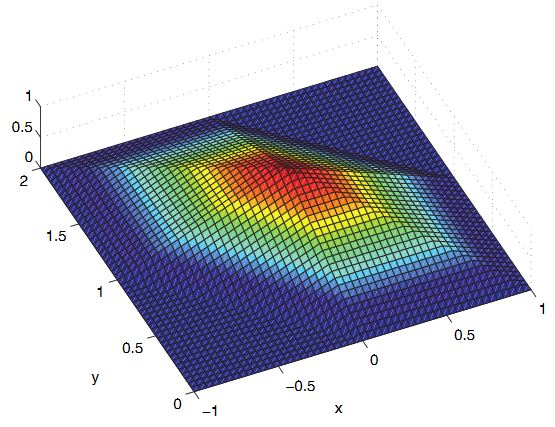
\includegraphics[width=0.46\textwidth]{Immagini/elementofinito.jpg}  
   }
	\subfigure[B-splines (tempo)]
   {
   \label{fig:basit}
	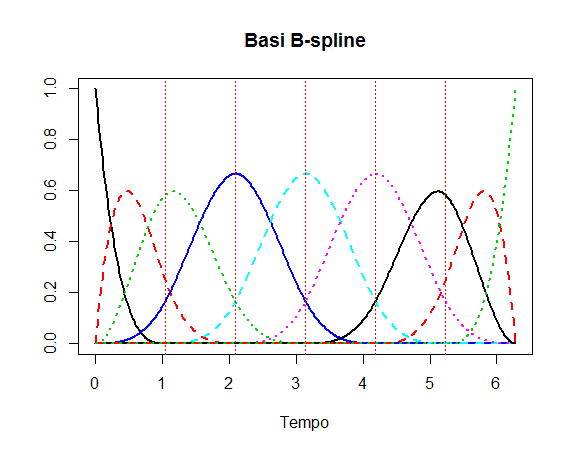
\includegraphics[width=0.46\textwidth]{Immagini/Bsplines.png}
   }
	\caption{Funzioni di base implementate nel codice}
	\label{fig:basi}
\end{figure}

Le basi in tempo a disposizione sono le B-splines, funzioni che, fissato un intervallo temporale e alcuni nodi in esso contenuti (nel nostro caso equispaziati), sono usate per l'espansione in base delle \textit{funzioni spline}. Il codice necessario è già stato implementato ed ottimizzato nel pacchetto \textit{fda} ed è stato riciclato per il codice del modello ST-PDE. In fig. \ref{fig:basit} sono riportate le 9 B-splines cubiche definite sull'intervallo $[0,2\pi]$ (che sarà usato per l'applicazione al dominio a forma di C). L'unico vincolo imposto a queste funzioni di base è il grado, che deve essere almeno 3 per avere la derivata seconda delle basi necessaria per la penalizzazione.

\section{Schematizzazione dell'algoritmo di stima}
L'esecuzione del codice è stata divisa in alcuni passi per poter permettere all'utente di inserire gradualmente gli oggetti in ingresso e fissare i parametri che servono per ottenere la stima finale. In più punti si è cercato di nascondere all'utente le variabili temporanee e di includere in opportune classi di R tutte le informazioni riguardanti concetti tra di loro comuni. 

Innanzitutto si ha l'acquisizione dei dati (e delle eventuali covariate) e la creazione della triangolazione. In questo caso non sono state implementate funzioni apposite poiché ci sono già pacchetti specializzati (nelle applicazioni che saranno presentate in seguito si è fatto uso di \textit{RTriangle} per la triangolazione).

Dopo aver definito i punti, la triangolazione e gli istanti di tempo occorre fissare le funzioni di base. Sono state implementate due funzioni di R, una per lo spazio e una per il tempo, che in base ai parametri in ingresso e agli ordini scelti per le funzioni di base creano appositi oggetti che memorizzano tutte le informazioni necessarie.  

A questo punto si ha la ricerca i migliori parametri di smoothing: definiti un insieme discreto di valori per $\lambda_S$ ed uno analogo su $\lambda_T$, l'indice in eq. \ref{eq:GCV} è minimizzato sul prodotto cartesiano di tali insiemi. Per una corretta applicazione del modello questa operazione deve essere ripetuta più volte, fino al raggiungimento di una accettabile precisione nella stima di $\underline{\lambda}$. Sono state implementate due funzioni, una per il caso senza covariate e una per il caso con covariate, a causa della diversità della \textit{smoothing matrix}. Questo è il passaggio più lento dell'algoritmo.

Dopo aver fissato i parametri di smoothing si arriva al cuore dell'algoritmo, poiché è calcolata la stima della soluzione. Ciò che eseguono le apposite funzioni è calcolare tutte le matrici di passaggio ($P$ e $B$) nascondendole all'utente e risolvere gli appositi sistemi lineari (eq. \ref{eq:sysnocovar}, \ref{eq:syscovar1} e \ref{eq:syscovar2}). In uscita è restituito un oggetto che racchiude i vettori ricavati e le funzioni di base, in modo da poter immagazzinare insieme tutti gli elementi necessari per tracciare grafici riguardanti la soluzione.

Terminata la stima, ciò che resta da fare è analizzare i risultati. Sono state create più funzioni, da scegliere in base a quello che si vuole visualizzare: calcolo della soluzione in punti ed istanti scelti, plot della funzione ad un istante fissato o ad un punto spaziale fissato, calcolo degli intervalli di confidenza approssimati (senza il termine di distorsione) per le componenti di $\underline{\beta}$.

\section{Strutture dati adottate}
Al momento dell'implementazione del codice corrispondente alle eq. \ref{eq:GCV}, \ref{eq:sysnocovar}, \ref{eq:syscovar1} e \ref{eq:syscovar2} è stato necessario decidere la corretta struttura dati per le matrici e una buona tecnica di inversione. In generale, quando si studiano dati distribuiti in spazio e tempo su domini complessi, le dimensioni delle matrici da invertire per calcolare $\hat{\underline{c}}$ sono di grandi dimensioni. Inoltre, a causa delle funzioni di base scelte in precedenza, le matrici $\Psi$, $\Phi$, $P_S$, $R_0$ e $R_1$ risulteranno sparse con molta facilità. Quindi la scelta di una struttura dati efficiente tra quelle disponibili in R è abbastanza delicata.

Sono stati analizzati quattro casi, in base al tipo di matrici (le matrici base di R o le sparse del pacchetto \textit{Matrix}) o alla tecnica di inversione (classica di R o con fattorizzazione QR). Sono stati misurati i tempi di calcolo della stima con queste quattro modalità nell'applicazione del dominio a forma di C senza covariate (sarà discusso nel dettaglio nel prossimo capitolo) e in tab. \ref{tab:tempo} sono riportati i risultati. Sono stati eseguiti più tentativi, al variare del numero di punti interni del dominio (e quindi della dimensione della matrice da invertire in \ref{eq:sysnocovar}), per poter controllare la velocità di esecuzione a difficoltà crescente.
\newline
\begin{table}[h]
\renewcommand{\arraystretch}{1.3}
\setlength{\tabcolsep}{2mm}
\centering
	\begin{tabular}{!{\vrule width 1.2pt}c!{\vrule width 1.2pt}c!{\vrule width 1pt}c!{\vrule width 1pt}c!{\vrule width 1pt}c!{\vrule width 1.2pt}}
	\noalign{\hrule height 1.2pt}
	Dimensione  & Classico & Classico+QR & Sparse & Sparse+QR \\
	\noalign{\hrule height 1pt}
	1446 & 11.89 & 15.33 & 31.48 & 1508.63 \\
	\noalign{\hrule height 1pt}
	2124 & 36.68 & 46.04 & 141.11 &  \\
	\noalign{\hrule height 1pt}
	3672 & 211.32 & 248.36 & 1369.21 & \\
	\noalign{\hrule height 1pt}
	7086 & 1592.88 & 1840.64 &  & \\
	\noalign{\hrule height 1.2pt}
	\end{tabular}
\caption{Tempo di calcolo della stima di $\protect\hat{\protect\underline{c}}$ (in secondi) nelle simulazioni eseguite sul dominio a forma di C}
\label{tab:tempo}
\end{table}
\newline
Non sono state eseguite più misurazioni per caso perchè già da queste è chiaro quale sia la miglior scelta. L'uso delle matrici sparse è stato progressivamente abbandonato poichè nettamente più lento. Anche la fattorizzazione QR non ha portato ad un miglioramento, perciò è stato adottata l'inversione base di R.

Il motivo di questa lentezza è legato al linguaggio di programmazione. Non è una novità che R non sia uno dei linguaggi maggiormente efficienti. Inoltre, tra tutte le operazioni a disposizione, l'esecuzione dei cicli e di operazioni di accesso è un punto debole\footnote{si consultino le considerazioni in questa pagina: \href{http://adv-r.had.co.nz/Rcpp.html}{http://adv-r.had.co.nz/Rcpp.html}}. Quindi l'uso di fattorizzazione QR (e della risoluzione di un sistema tramite \textit{backward substitutions} che richiede) o di matrici sparse (implementate tramite tre vettori rispettivamente con indici di riga, colonna e valori non nulli) sono necessariamente lente per l'alto numero di cicli che richiedono. Le funzioni base di R, invece, sono certamente più ottimizzate. La conseguenza di questa analisi sarà riportata anche nel cap. \ref{cap:conclusione}, in cui si sottolinea che l'integrazione con linguaggi più efficienti nei colli di bottiglia del codice porterebbe a miglioramenti computazionali sicuri e alla possibilità di applicazione a dataset di grandi dimensioni.

\chapter{Simulazioni nel caso del dominio a forma di C}
\label{cap:domC}
Prima di applicare il modello ST-PDE all'analisi della produzione di rifiuti nella provincia di Venezia sono state eseguite simulazioni su un caso noto e più semplice. Si è scelto di analizzare il dominio a forma di C e la corrispondente funzione spaziale $g(\underline p)$ (riportata in fig. \ref{fig:domC_fstest}) descritti in \cite{art:ramsay}, \cite{art:sangalli}, \cite{art:wood} e implementata nel pacchetto R \textit{mgcv}. La funzione $g(\underline p)$ è solo spaziale, quindi è stata introdotta una variazione temporale deformando con il coseno:
$$
f(\underline p, t)=g(\underline p)cos(t)
$$
Su questo semplice caso sono stati eseguiti i primi tentativi per il modello ST-PDE sia senza covariate che con una covariata generata.
\begin{figure}[h]
	\centering
	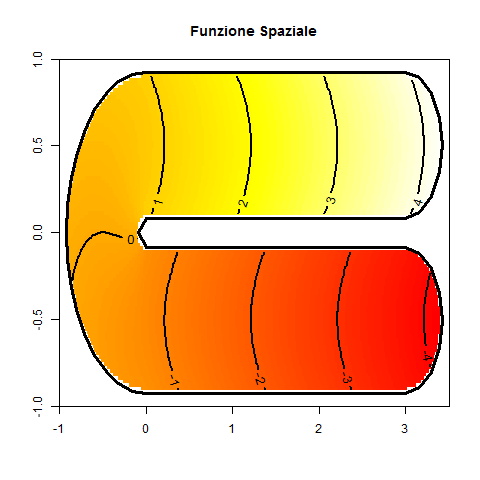
\includegraphics[width=0.44\textwidth]{Immagini/DomCinizio/DomC_fstest.png}   
	\caption{Funzione spaziale $g(\protect\underline{p})$}
	\label{fig:domC_fstest}
\end{figure}
\newpage
Dalla rappresentazione di $g(\underline p)$ si può notare come sia fondamentale la geometria del problema, come per il caso della produzione dei rifiuti nella provincia di Venezia. Infatti, i massimi e i minimi si trovano sulle estremità del dominio, tra di loro vicine ma non collegate se non attraverso tutto il dominio.

\section{Triangolazione e istanti temporali}
In questo caso non sono presenti punti spaziali definiti dalla natura del problema (come possono essere i comuni per la provincia di Venezia), quindi è stato necessario ricavarli. Sono stati generati casualmente 150 punti all'interno del rettangolo $[-1,+3.5] \times [-1,+1]$ e di questi sono stati considerati validi solo quelli che ricadevano all'interno del dominio. Non è stata usata la descrizione della frontiera presente in \textit{mgcv}, ma una versione diversa che permette di avere punti anche nella parte rettilinea del bordo.
\begin{figure}[t]
	\centering
	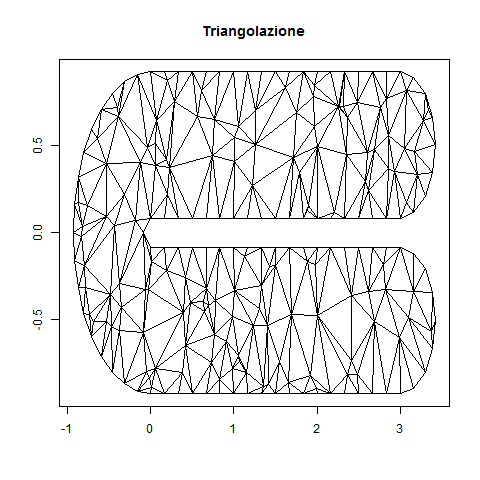
\includegraphics[width=0.44\textwidth]{Immagini/DomCinizio/DomC_Triangolazione.png}
	\caption{Triangolazione del dominio a forma di C}
	\label{fig:domC_triang}
\end{figure}
In fig. \ref{fig:domC_triang} è riportata la triangolazione di Delaunay ottenuta grazie al pacchetto R \textit{RTriangle}. Come basi in spazio sono stati usati gli elementi finiti lineari definiti su questa triangolazione. In tutti gli esempi che seguiranno sarà considerata questa descrizione del dominio, che è formata da 241 punti (pari anche al numero di basi spaziali $N$). Di questi, 108 sono di frontiera e i restanti 133 corrispondono agli $n$ punti sui quali saranno disponibili i dati.

Come intervallo temporale di variazione dei dati è stato scelto $[0,2\pi]$ per sfruttare la periodicità del coseno. All'interno di questo intervallo sono stati ricavati 9 istanti temporali equidistanti tra di loro, quindi uno ogni $\frac{\pi}{4}$. Sono state fissate come basi in tempo le B-splines cubiche. Il numero di basi $M$ è uguale al numero di istanti temporali a disposizione $m$, quindi 9. 
\newpage
\section{Caso senza covariata}

Nei punti e negli istanti temporali disponibili i dati sono stati ricavati dalla funzione esatta con l'aggiunta del rumore:
$$
z_{ij}=g(\underline p_{i})cos(t_j) + \varepsilon_{ij} \qquad \forall i \in 1\ldots n, \forall j \in 1\ldots m
$$
dove
$$
\varepsilon_{ij}\stackrel{\mathrm{iid}}{\sim}N(0,0.5^2) \qquad \forall i \in 1\ldots n, \forall j \in 1\ldots m \ .
$$

Per poter eseguire una analisi ottimale, come primo passo è necessario scegliere i valori dei parametri di smoothing ottimizzando l'indice $\mathrm{GCV}(\underline \lambda)$ riportato in eq. \ref{eq:GCV}. In queste analisi $\lambda_S$ e $\lambda_T$ saranno sempre espressi in potenze di 10. Per trovare dei buoni valori per i parametri sono stati eseguiti più tentativi, creando due insiemi discreti di variazione per $\log_{10}\lambda_S$ e $\log_{10}\lambda_T$ e minimizzando sui $\underline \lambda$ corrispondenti al prodotto cartesiano tra di essi. Il procedimento viene ripetuto qualche volta rendendo la griglia sempre più fitta. Dopo alcune iterazioni, è stato fissato $\underline \lambda = (10^{-0.375}, 10^{-3.25})$ come valore definitivo per questa analisi ed è stata calcolata computazionalmente la stima.

In fig. \ref{fig:DomC_ris} sono riportati i confronti tra funzione reale e stimata nei primi istanti di tempo (la scala di colori è stata resa uniforme tra tutti i grafici). Si può notare come la funzione stimata sia effettivamente molto simile a quella reale. La diversità tra le due estremità del dominio è stata colta, poiché il procedimento ha considerato correttamente la definizione della geometria spaziale.
\newpage
\begin{figure}[H]
\centering
	\subfigure[Funzione reale a $t=0$]
   {
	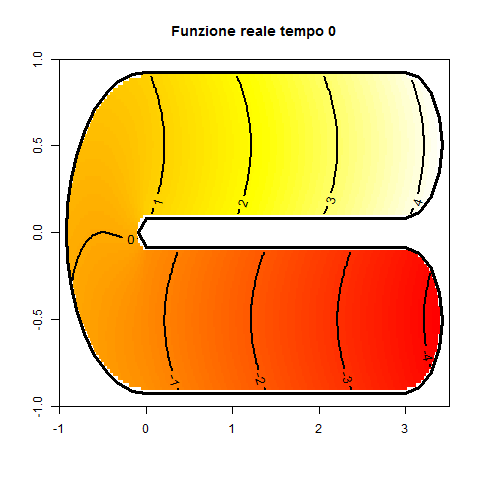
\includegraphics[width=0.40\textwidth]{Immagini/DomC/DomC_0reale.png}   
   }
	\subfigure[Funzione stimata a $t=0$]
   {
	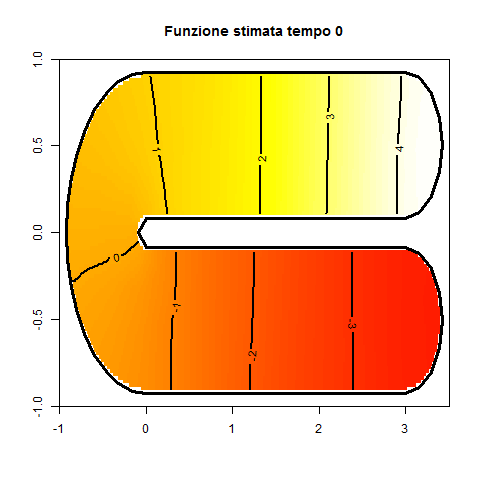
\includegraphics[width=0.40\textwidth]{Immagini/DomC/DomC_0stimata.png}
   }
   \subfigure[Funzione reale a $t=\frac{\pi}{4}$]
   {
	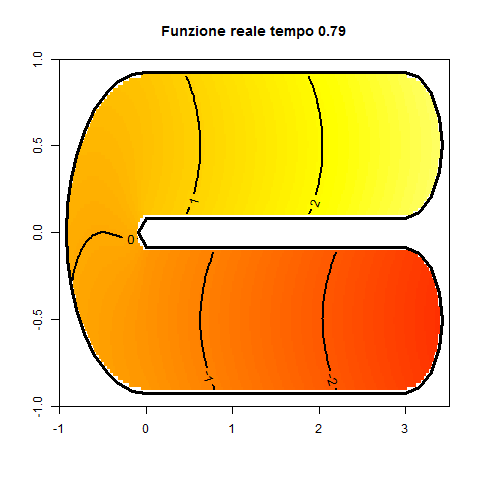
\includegraphics[width=0.40\textwidth]{Immagini/DomC/DomC_1reale.png}   
   }
	\subfigure[Funzione stimata a $t=\frac{\pi}{4}$]
   {
	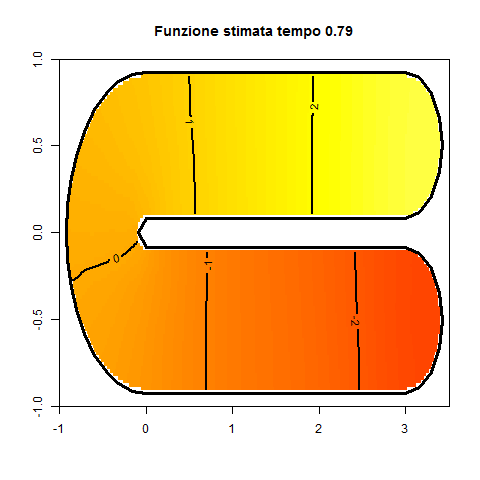
\includegraphics[width=0.40\textwidth]{Immagini/DomC/DomC_1stimata.png}
   }
   \subfigure[Funzione reale a $t=\frac{\pi}{2}$]
   {
	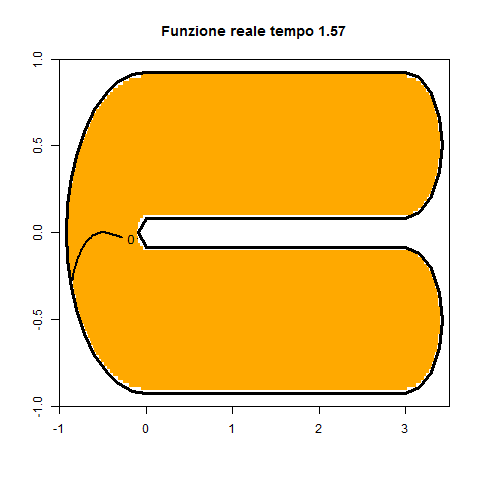
\includegraphics[width=0.40\textwidth]{Immagini/DomC/DomC_2reale.png}   
   }
	\subfigure[Funzione stimata a $t=\frac{\pi}{2}$]
   {
	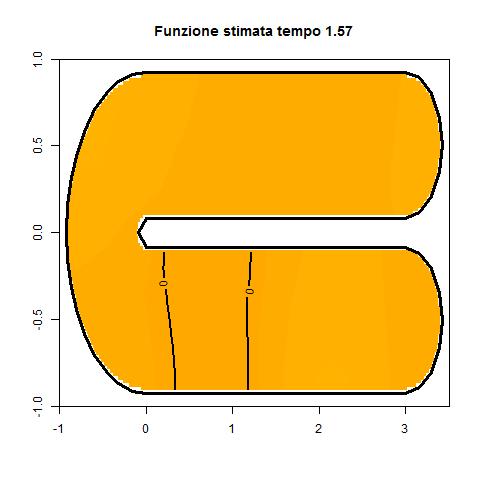
\includegraphics[width=0.40\textwidth]{Immagini/DomC/DomC_2stimata.png}
   }
	\caption{Stime della funzione $f(\protect\underline{p},t)$ ad alcuni istanti di tempo, caso senza covariata}
	\label{fig:DomC_ris}
\end{figure}
\newpage
In fig. \ref{fig:DomC_ris2} si ha il confronto dell'evoluzione temporale in alcuni nodi della triangolazione. Oltre alla curva stimata è stata tracciata la reale, che è una cosinusoide di ampiezza nota (grazie alla perfetta conoscenza di $g(\underline p)$) riportata con i grafici. I punti rossi corrispondono al dato generato (termine dovuto al rumore compreso). Tanto più è vicina a zero l'ampiezza della curva, tanto più il rumore influenza la stima poiché più rilevante (infatti, in fig. \ref{fig:DomC_ris}, le curve di livello della funzione stimata sono le più diverse da quelle reali quando la stima è vicina a zero). Tuttavia, anche nel caso di ampiezza vicina al valore massimo di $g(\underline p)$ in fig. \ref{fig:DomC_ris2C}, l'andamento del fenomeno è stato riconosciuto e non è stata ottenuta una stima troppo interpolante dei dati. Si può concludere che la stima è molto buona, sebbene leggermente più confusa nella parte centrale del dominio.

\begin{figure}[t]
	\centering
	\subfigure[Ampiezza $0.3486$]
	{
	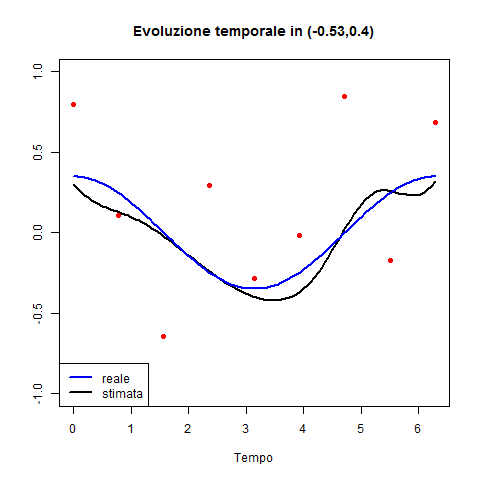
\includegraphics[width=0.31\textwidth]{Immagini/DomC/tfissato1.png}   
   }
	\subfigure[Ampiezza $1.3819$]
   {
	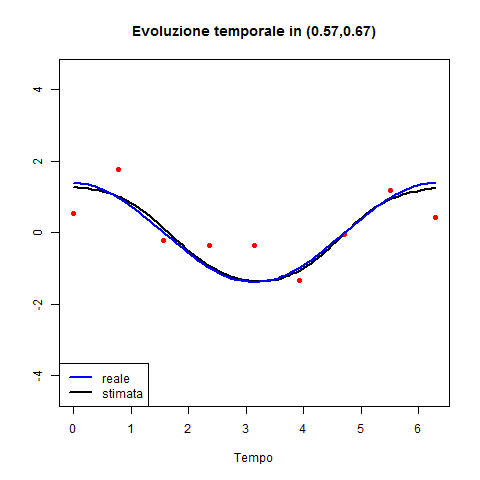
\includegraphics[width=0.31\textwidth]{Immagini/DomC/tfissato2.png}
   }
   \subfigure[Ampiezza $4.1648$]
   {
	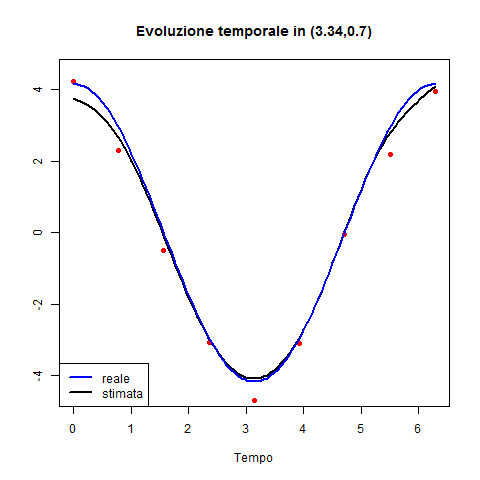
\includegraphics[width=0.31\textwidth]{Immagini/DomC/tfissato3.png}  
	\label{fig:DomC_ris2C} 
   } 
	\caption{Evoluzione temporale in alcuni nodi della triangolazione, caso senza covariata}
	\label{fig:DomC_ris2}
\end{figure}
\newpage
\section{Caso con covariata}

Nel problema della stima della funzione $f(\underline p,t)=g(\underline p)cos(t)$ non sono presenti covariate. Quindi per poter testare il modello anche in questo caso, è stato necessario generare valori da assumere come covariata in ogni punto spaziale ed istante temporale in cui si ha la risposta.
In definitiva i dati sono così formati:
$$
z_{ij}=g(\underline p_{i})cos(t_j) + \beta w_{ij} + \varepsilon_{ij} \qquad \forall i \in 1\ldots n, \forall j \in 1\ldots m
$$
dove covariata e rumore sono generate da due normali tra loro indipendenti:
$$
w_{ij}\stackrel{\mathrm{iid}}{\sim}N(0,1) \qquad \forall i \in 1\ldots n, \forall j \in 1\ldots m
$$
$$
\varepsilon_{ij}\stackrel{\mathrm{iid}}{\sim}N(0,0.5^2) \qquad \forall i \in 1\ldots n, \forall j \in 1\ldots m
$$
e $\beta$ è fissato a 1. Se il modello è buono, c'è da aspettarsi che la parte di funzione stimata senza covariata sia vicina a $f(\underline p,t)$ e che $\hat{\beta}$ si avvicini a 1.
 
Anche in questo caso è necessaria una analisi preliminare per fissare i valori di $\underline \lambda$ ottimizzando l'indice $\mathrm{GCV}(\underline \lambda)$, che nel caso con covariata si differenzia dal precedente solo per la forma della \textit{smoothing matrix}. Dopo alcuni tentativi su griglie discrete (esattamente come nel caso precedente) è stato ottenuto un minimo in corrispondenza di $\underline \lambda = (10^{-0.125}, 10^{-3.25})$. 
\newpage
\begin{figure}[H]
\centering
\subfigure[Funzione reale a $t=0$]
   {
	\includegraphics[width=0.40\textwidth]{Immagini/DomCCovar/DomCcovar_0reale.png}   
   }
\subfigure[Funzione stimata a $t=0$]
   {
	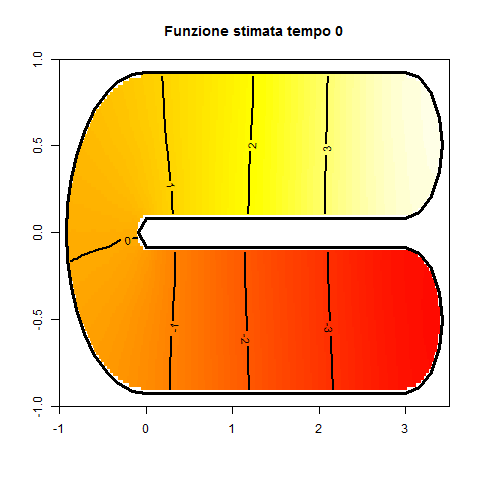
\includegraphics[width=0.40\textwidth]{Immagini/DomCCovar/DomCcovar_0stimata.png}
   }
\subfigure[Funzione reale a $t=\frac{\pi}{4}$]
   {
	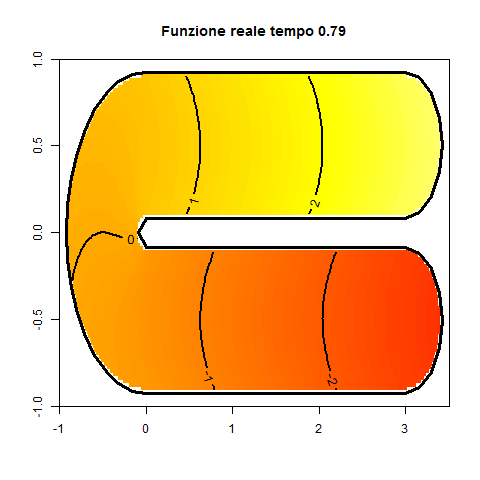
\includegraphics[width=0.40\textwidth]{Immagini/DomCCovar/DomCcovar_1reale.png}   
   }
\subfigure[Funzione stimata a $t=\frac{\pi}{4}$]
   {
	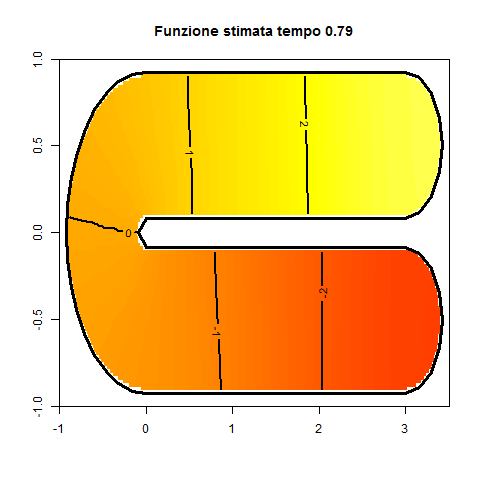
\includegraphics[width=0.40\textwidth]{Immagini/DomCCovar/DomCcovar_1stimata.png}
   }
\subfigure[Funzione reale a $t=\frac{\pi}{2}$]
   {
	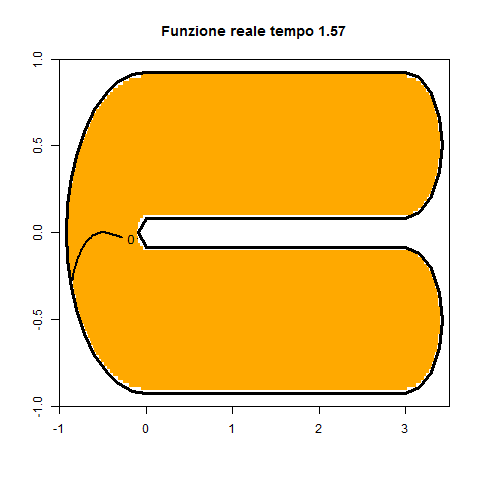
\includegraphics[width=0.40\textwidth]{Immagini/DomCCovar/DomCcovar_2reale.png}   
   }
\subfigure[Funzione stimata a $t=\frac{\pi}{2}$]
   {
	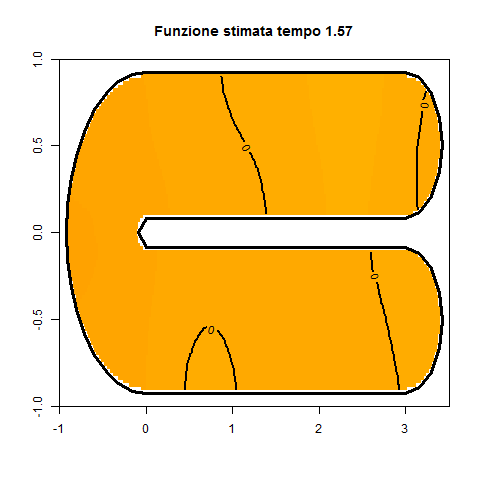
\includegraphics[width=0.40\textwidth]{Immagini/DomCCovar/DomCcovar_2stimata.png}
   }
\caption{Stime della funzione $f(\protect\underline{p},t)$ ad alcuni istanti di tempo, caso con covariata}
\label{fig:DomCcovar_ris}
\end{figure}
\newpage
In fig. \ref{fig:DomCcovar_ris2}, analogamente a quanto fatto nel caso senza covariata, si hanno i grafici dell'evoluzione temporale della funzione in alcuni punti spaziali. I punti rossi tracciati corrispondono alla parte di dato senza il termine dovuto alla covariata (ma con il rumore). Le conclusioni sono le stesse del caso senza covariata: la stima è ben riuscita e la vera variazione temporale è stata colta dal modello. Tuttavia, avvicinandosi alla parte centrale del dominio, si ha una maggiore influenza del rumore, in questo caso meno evidente a causa della presenza della covariata.

\begin{figure}[t]
	\centering
	\subfigure[Ampiezza $0.2810$]
	{
	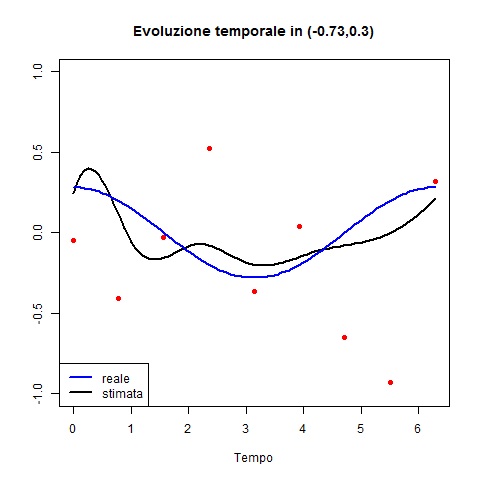
\includegraphics[width=0.31\textwidth]{Immagini/DomCCovar/tfissato1.png}   
   }
	\subfigure[Ampiezza $1.2761$]
   {
	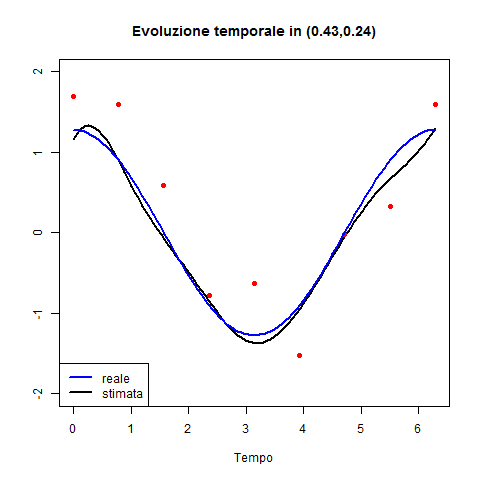
\includegraphics[width=0.31\textwidth]{Immagini/DomCCovar/tfissato2.png}
   }
   \subfigure[Ampiezza $3.8577$]
   {
	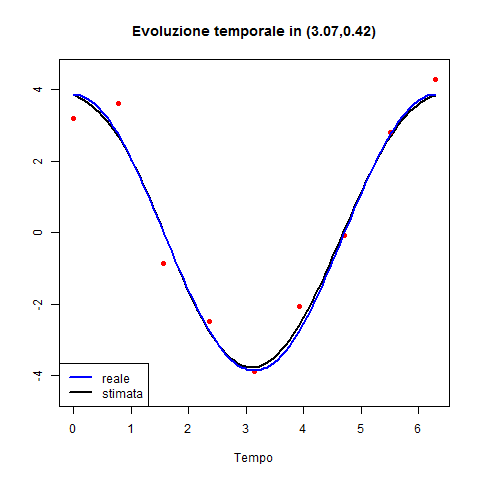
\includegraphics[width=0.31\textwidth]{Immagini/DomCCovar/tfissato3.png}   
   } 
	\caption{Evoluzione temporale in alcuni nodi della triangolazione, caso con covariata}
	\label{fig:DomCcovar_ris2}
\end{figure}

Dai grafici precedenti si può concludere che la stima della parte funzionale della risposta sia effettivamente una buona approssimazione della reale. Occorre verificare, però, anche che il contributo della covariata sia ben riconosciuto dal modello, controllando il valore stimato di $\beta$. Si ha:
$$
\hat{\beta} \approx 1.005 \ ,
$$
valore vicinissimo al reale. Pertanto è interessante validare questo risultato attraverso un test del tipo
$$
\begin{cases}
H_0: & \beta=1 \\
H_1: & \beta \not = 1
\end{cases} \ ,
$$
per poter verificare con una data significatività se il valore stimato corrisponde a quello reale. Per poter fare ciò si costruisce un un intervallo di confidenza approssimato al $95\%$ per $\beta$ (eliminando il termine di distorsione) con quanto ricavato in sez. \ref{sec:IC}. Ne risulta:
$$
\beta \in [0.9843;1.0259]
$$
che contiene 1. L'ipotesi $H_0$ può essere accettata.
\newpage
Concludendo, la simulazione esposta in questo capitolo ha permesso di verificare, in un caso dalle caratteristiche totalmente note e con una forte dipendenza dalla geometria spaziale, l'appropriata stima del campo spazio-temporale e del termine con covariata. Grazie a questi risultati (e alla possibilità di conoscere i valori reali su tutto il dominio) si può dedurre che questo esempio sia adatto per il confronto delle stime del modello ST-PDE con le altre tecniche disponibili in letteratura.
\newpage
\thispagestyle{empty}

\chapter{Confronto con altri metodi}
\label{cap:confronto}

Il modello ST-PDE, come è già stato evidenziato nel capitolo \ref{cap:panoramica}, non è l'unico modello disponibile per l'analisi funzionale di dati distribuiti sia in spazio che in tempo. Pertanto è necessario che sia confrontato con le altre principali metodologie presenti in letteratura, al fine di poter dire se e quanto tale modello possa rappresentare un miglioramento in questo campo. I confronti saranno eseguiti nel caso della simulazione sul dominio a forma di C, poiché la conoscenza della funzione reale permette il calcolo dell'errore di stima. 

Una tecnica da confrontare è senza dubbio il kriging spazio-temporale (KRIG). Le stime sono ottenute fissando un variogramma separabile e marginalmente esponenziale in spazio e tempo. I parametri del variogramma sono stimati dall'empirico e, successivamente, è possibile calcolare la stima grazie alle funzioni del pacchetto R \textit{gstat}. Per alcuni problemi con l'uso del pacchetto il kriging non sarà analizzato nel caso con covariata. Come è già stato evidenziato precedentemente, in questa tecnica non è preso in considerazione il dominio spaziale. Pertanto ci si aspettano stime peggiori rispetto ai metodi che possiedono questa caratteristica.

Assieme al modello costruito, in \cite{art:augustin} è possibile consultare il codice per il calcolo della stima, implementato nel pacchetto R \textit{mgcv}. Per un corretto confronto con il modello ST-PDE sarà considerato un solo termine funzionale per la risposta, costituito dal prodotto tensoriale dei modelli marginali in spazio e tempo (definiti dalle funzioni di base e dai termini di penalizzazione differenziali, analoghi a quelli proposti per ST-PDE). Saranno sempre considerate come basi in tempo le \textit{Regression splines} cubiche, mentre in spazio saranno
\newpage
\noindent analizzati due casi:
\begin{itemize}
\item basi spaziali per \textit{thin plate splines}, riportate in \cite{package:mgcv4}, che sono basi radiali non in grado di considerare la geometria spaziale (TPS);
\item basi spaziali per \textit{soap film smoothing}, analizzate nel dettaglio in \cite{art:wood} e utilizzate in \cite{art:marra} e \cite{art:augustin} e costituite da due insiemi di funzioni (rispettivamente per la parte interna del dominio e per la frontiera) appositamente pensate per casi con dominio spaziale complesso (SOAP).
\end{itemize}

La triangolazione e i dati sono gli stessi che sono stati usati nel capitolo \ref{cap:domC}. In aggiunta è stata costruita una griglia spazio-temporale di punti per la validazione, attraverso l'uso di 80 punti equispaziati in $[-1,+3.5]$, 40 punti in equispaziati $[-1,+1]$ e 20 istanti di tempo equispaziati in $[0,2\pi]$. Ovviamente l'errore è stato valutato soltanto sui punti che ricadevano all'interno del dominio a forma di C.

I modelli sono stati confrontati attraverso il Root Mean Square Error ($\mathrm{RMSE}$) calcolato nei punti di validazione. Quindi se se $V$ è l'insieme dei punti della griglia interni al dominio, fissato un modello si avrà:
$$
\mathrm{RMSE}_V=\sqrt{\frac{\sum_{(\underline p_i,t_i)\in V} (\hat{z}_{ij}-g(\underline p_i)cos(t_i))^2}{\mathrm{card}(V)}}
$$ 
Il procedimento è stato iterato 50 volte, per poter escludere possibili effetti particolari dovuti alla generazione del rumore.

\newpage
\section{Caso senza covariata}
Nel caso senza covariata si hanno i risultati riportati in fig. \ref{fig:cfr}, in cui sono stati tracciati i boxplot dei valori di $\mathrm{RMSE}$ ottenuti nelle 50 iterazioni per ogni metodo. Subito si nota che l'errore commesso è minore nel caso di ST-PDE, e quindi la stima ottenuta con il modello proposto è la migliore.

I risultati riflettono quanto è stato ipotizzato in precedenza: KRIG e TPS, che non considerano la geometria del problema, hanno prodotto gli errori più alti. Invece SOAP e ST-PDE commettono errori minori, ma tra i due il migliore è ST-PDE. Come ulteriore conferma di tutto ciò, in fig. \ref{fig:confronto_altri_metodi_nocov} sono riportate le stime ottenute dai differenti metodi per i primi istanti di tempo.  

\begin{figure}[t]
	\centering
	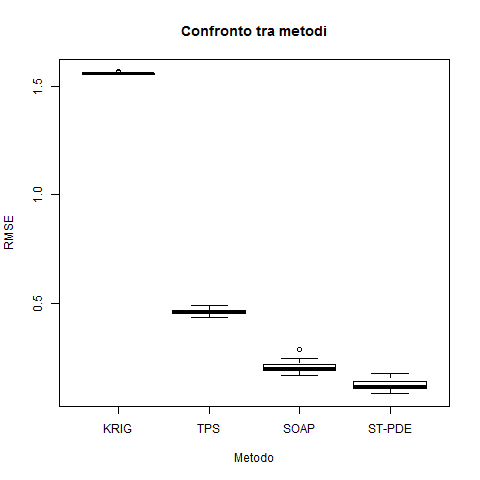
\includegraphics[width=0.60\textwidth]{Immagini/Confronto_metodi.png}   
	\caption{Confronto tra i metodi, caso senza covariata}
	\label{fig:cfr}
\end{figure}

\begin{landscape}
\begin{figure}
\centering
\begin{tabular}{lcccccc}
& Funzione reale & Dati generati & KRIG & TPS & SOAP & ST-PDE \\
&&&&&&\\
\parbox[t]{2mm}{\multirow{3}{*}{\rotatebox[origin=r]{90}{$t=0$}}}&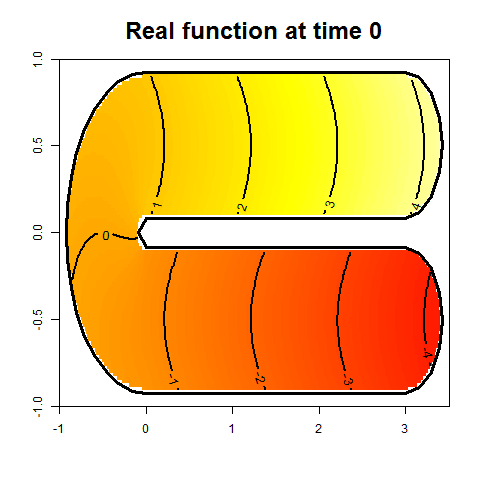
\includegraphics[trim=0cm 0cm 0cm 1.8cm,clip=true,width=0.19\textwidth,valign=t]{Immagini/simulazioni/REALEtempo1.png} &
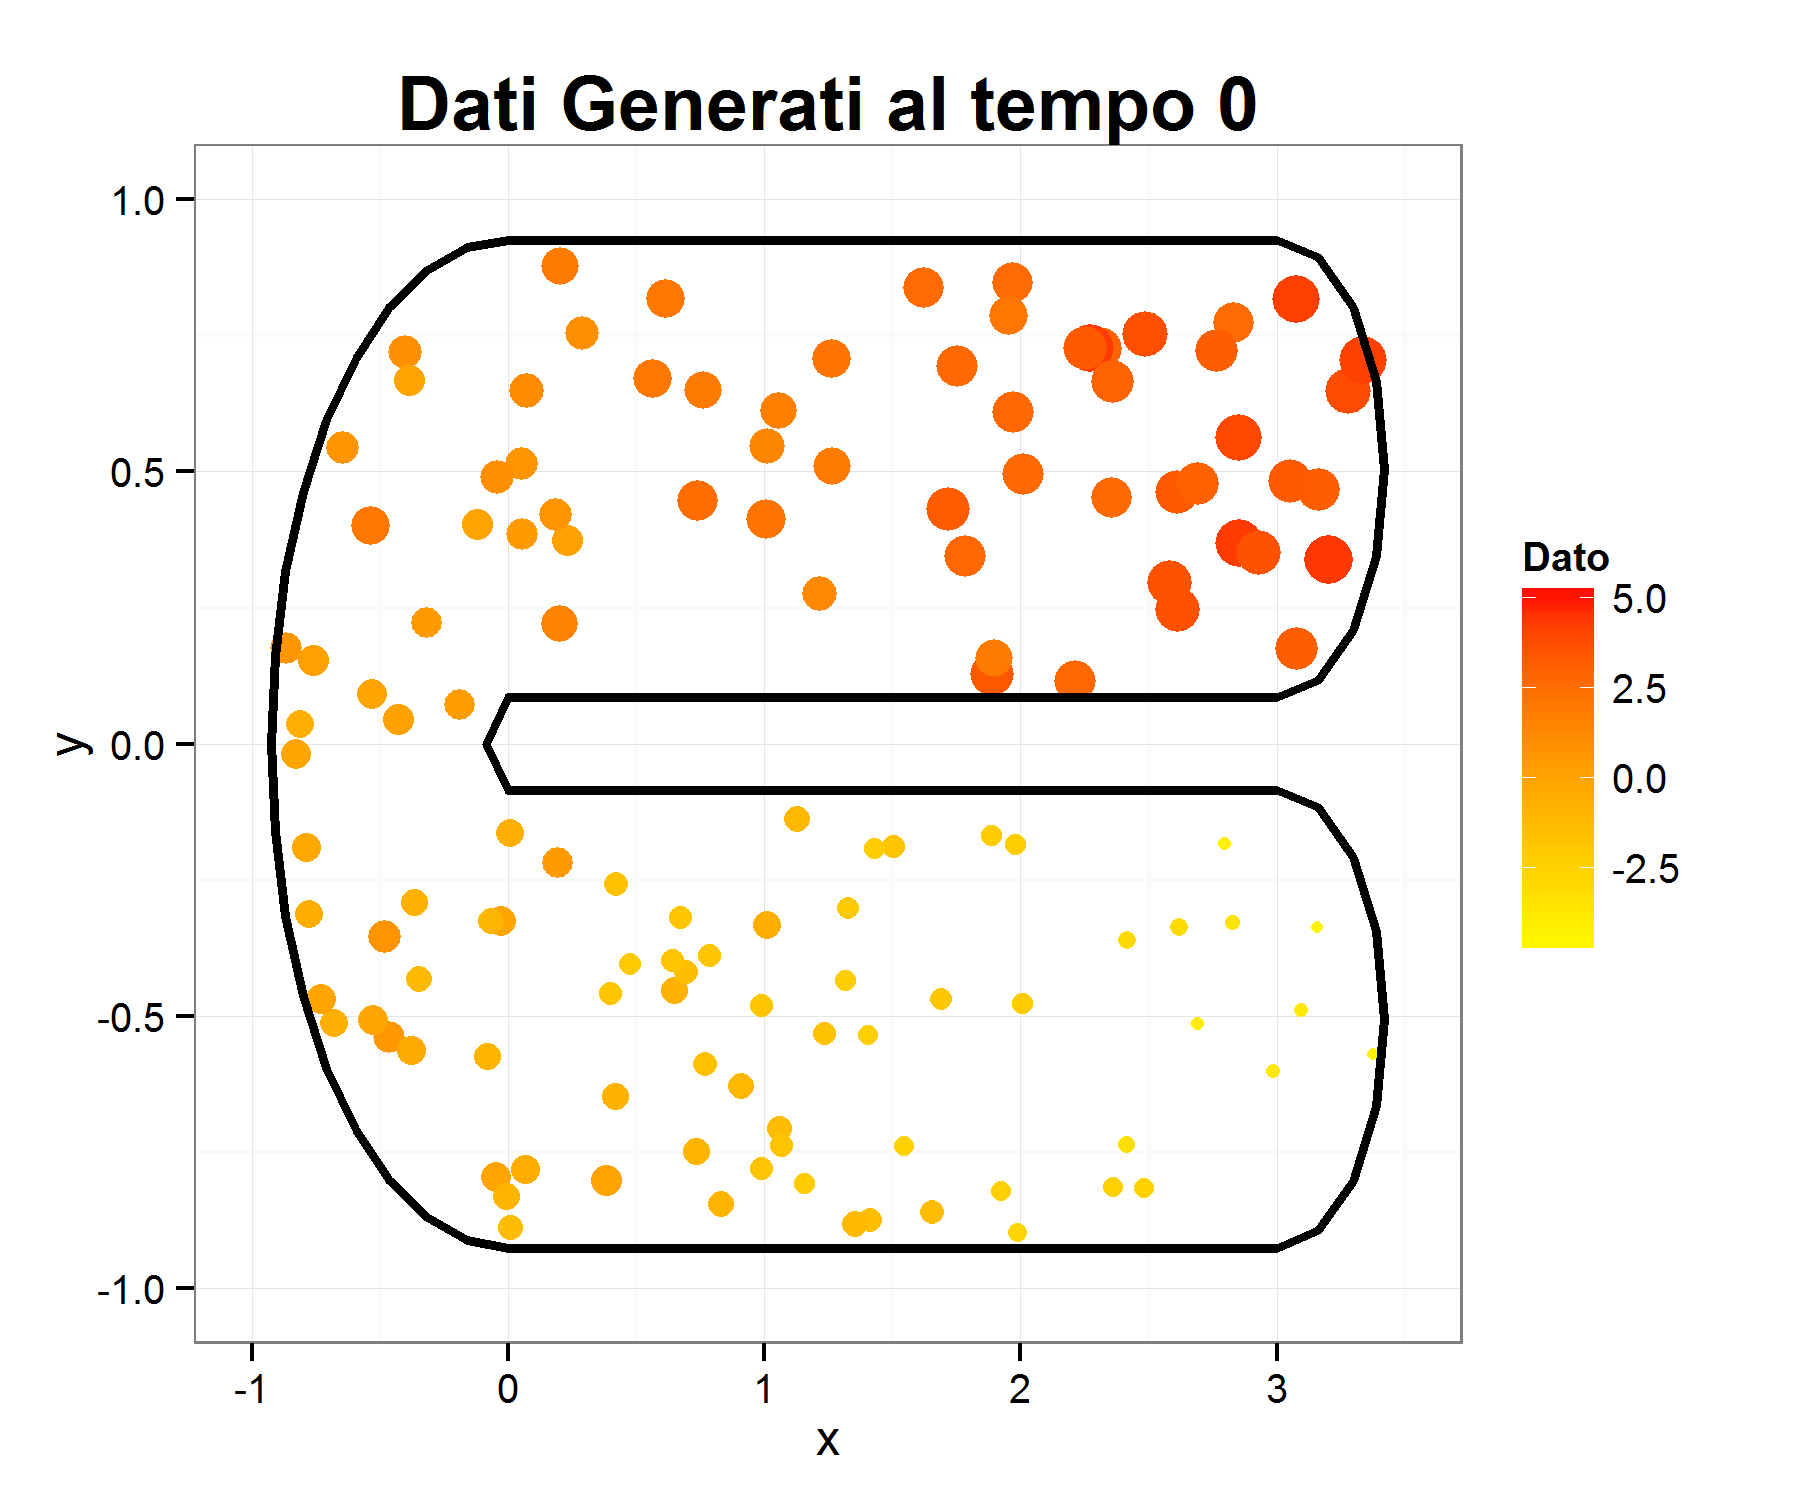
\includegraphics[trim=0.8cm 0.8cm 2.5cm 1.2cm,clip=true,width=0.19\textwidth,valign=t]{immagini/simulazioni/Dati_tempo1.png}&
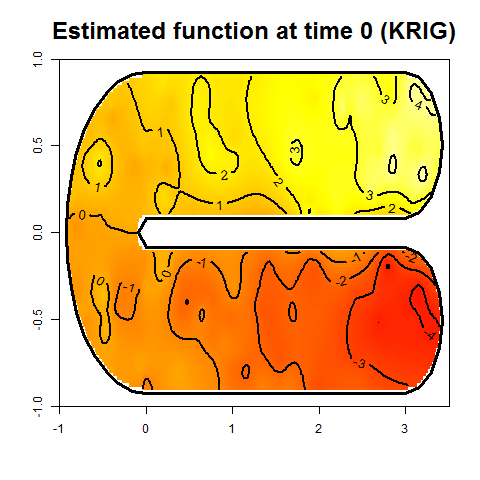
\includegraphics[trim=0cm 0cm 0cm 1.8cm,clip=true,width=0.19\textwidth,valign=t]{Immagini/simulazioni/KRIGtempo1.png}&
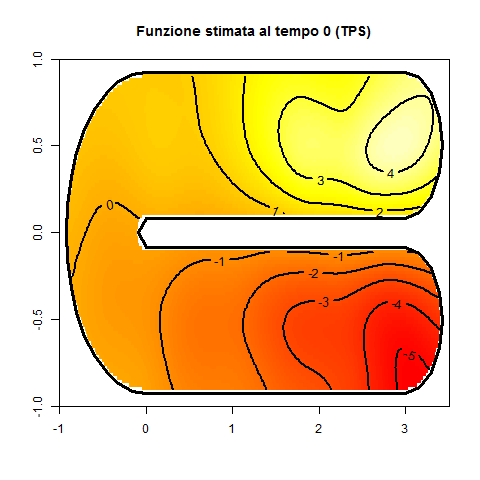
\includegraphics[trim=0cm 0cm 0cm 1.8cm,clip=true,width=0.19\textwidth,valign=t]{Immagini/simulazioni/TPStempo1.png}&
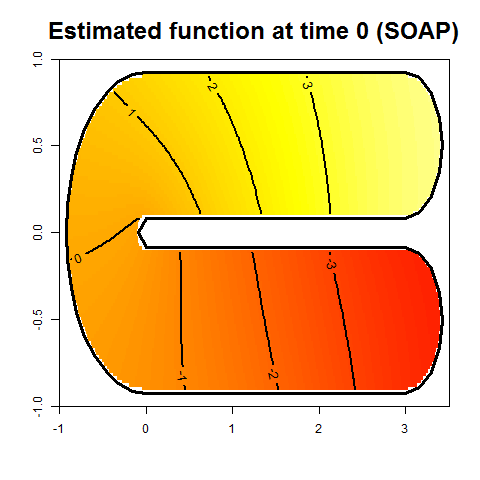
\includegraphics[trim=0cm 0cm 0cm 1.8cm,clip=true,width=0.19\textwidth,valign=t]{Immagini/simulazioni/SOAPtempo1.png}&
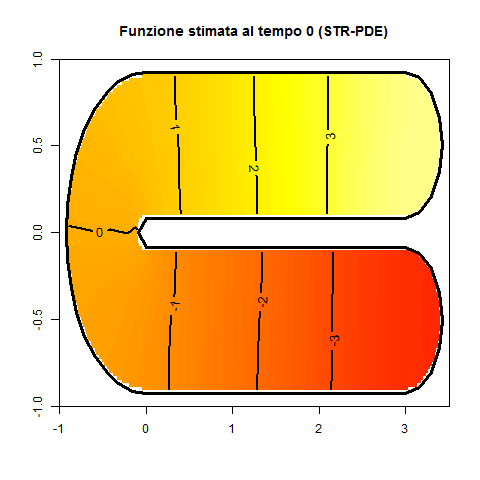
\includegraphics[trim=0cm 0cm 0cm 1.8cm,clip=true,width=0.19\textwidth,valign=t]{Immagini/simulazioni/STSRtempo1.png}\\
\parbox[t]{2mm}{\multirow{3}{*}{\rotatebox[origin=c]{90}{$t=0.785$}}}&
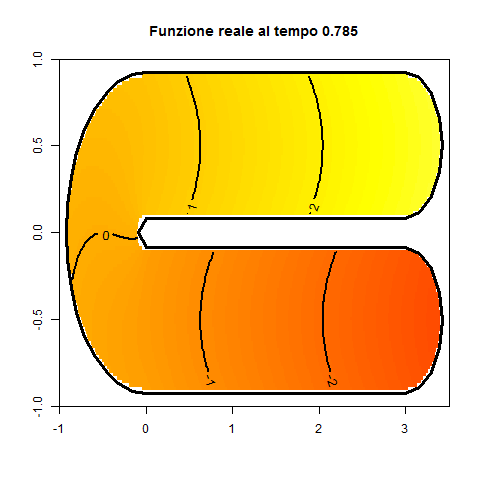
\includegraphics[trim=0cm 0cm 0cm 1.8cm,clip=true,width=0.19\textwidth,valign=t]{Immagini/simulazioni/REALEtempo2.png}&
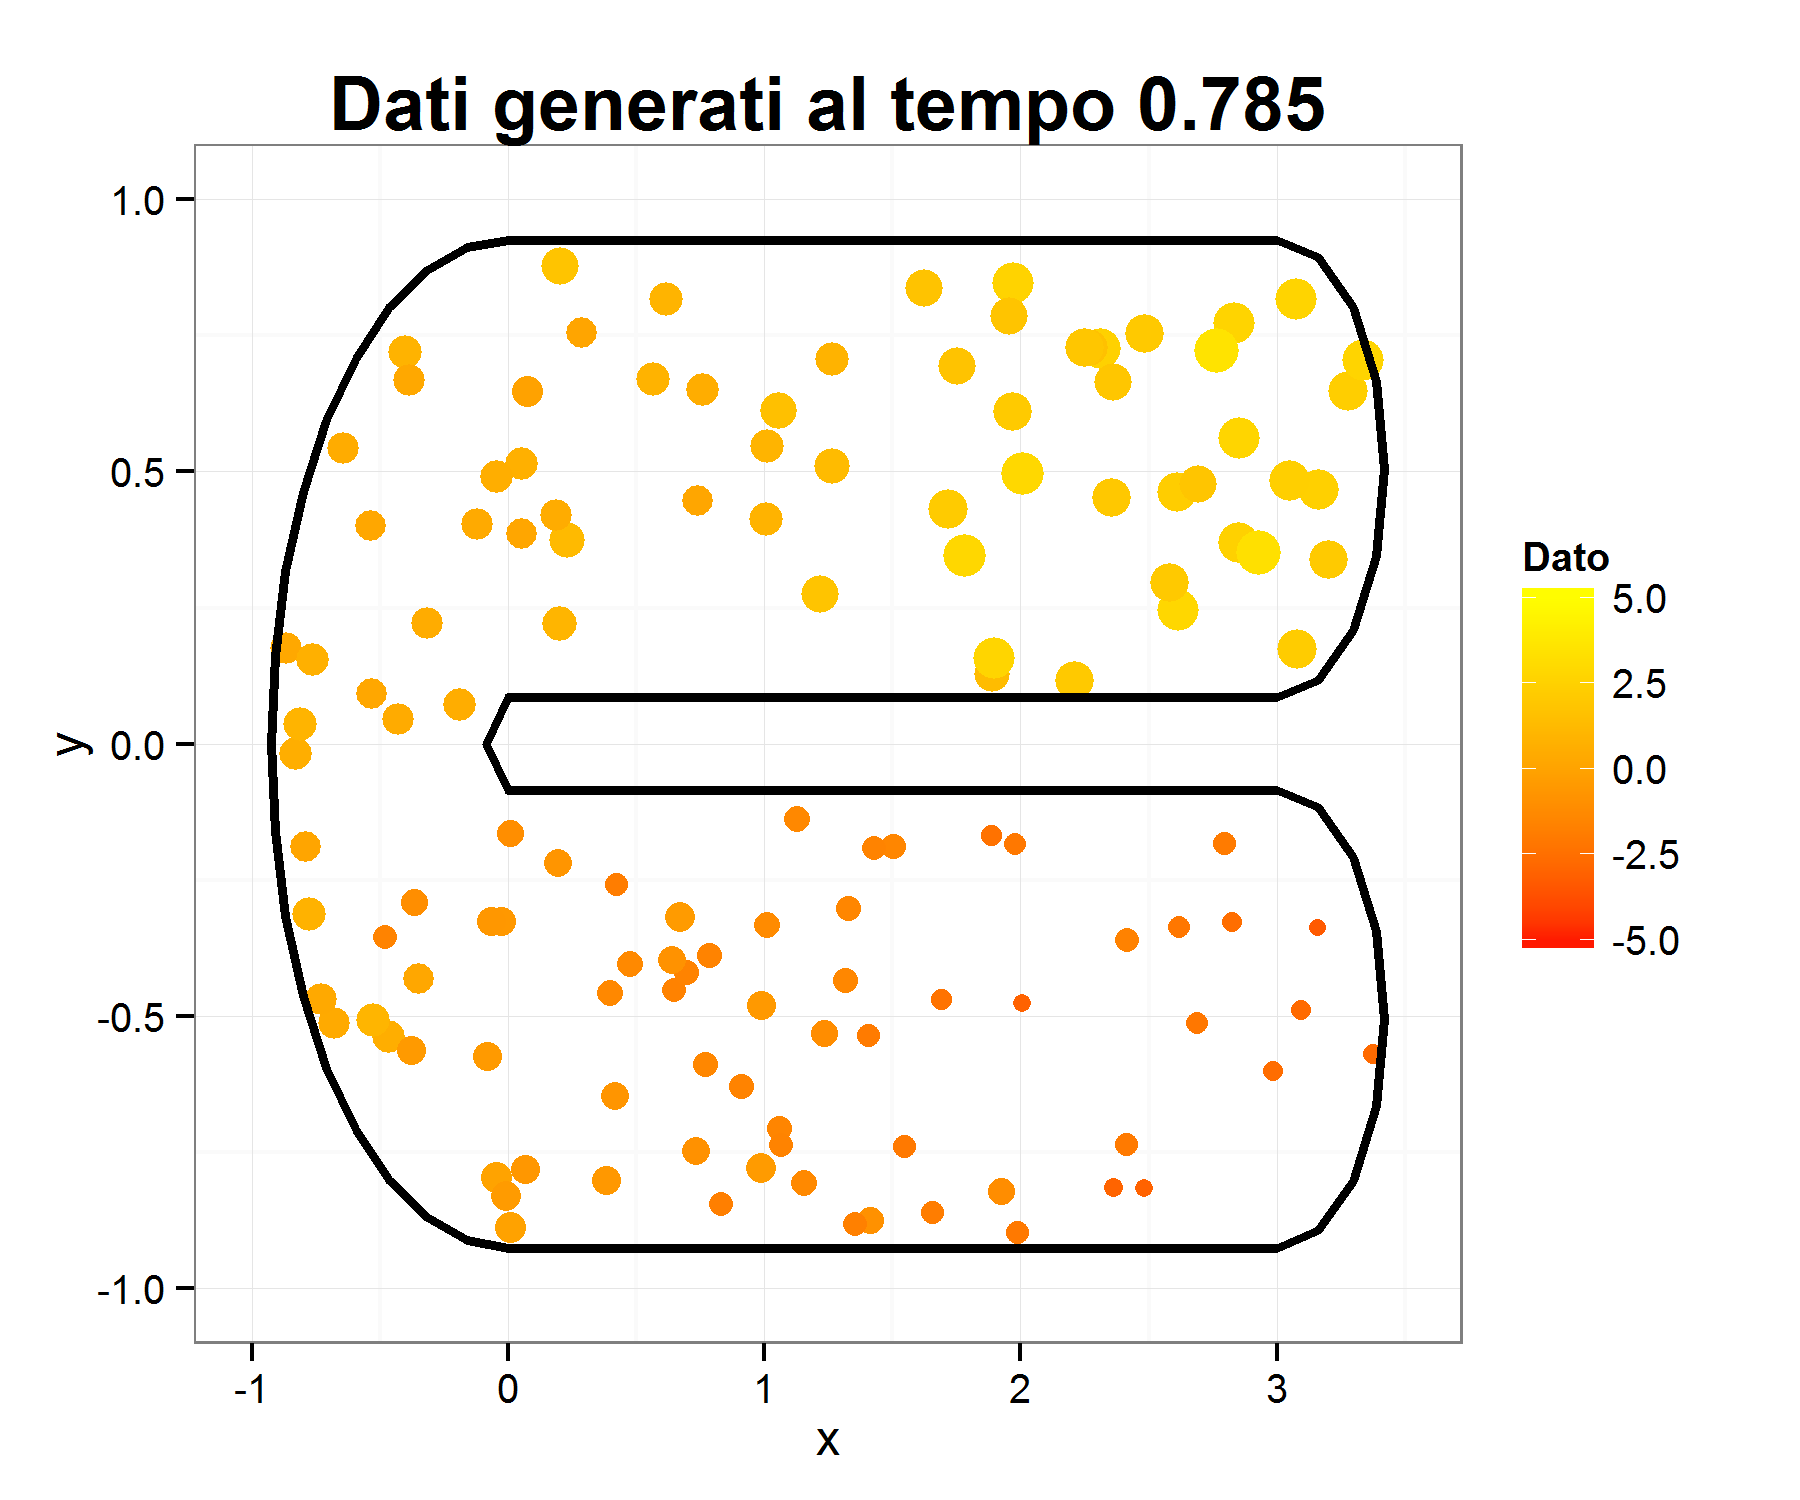
\includegraphics[trim=0.8cm 0.8cm 2.5cm 1.2cm,clip=true,width=0.19\textwidth,valign=t]{Immagini/simulazioni/Dati_tempo2.png}&
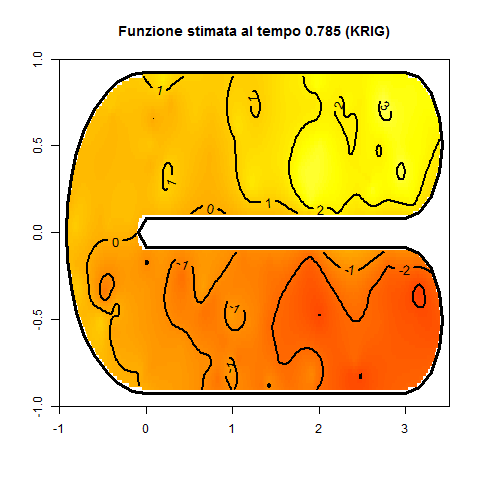
\includegraphics[trim=0cm 0cm 0cm 1.8cm,clip=true,width=0.19\textwidth,valign=t]{Immagini/simulazioni/KRIGtempo2.png}&
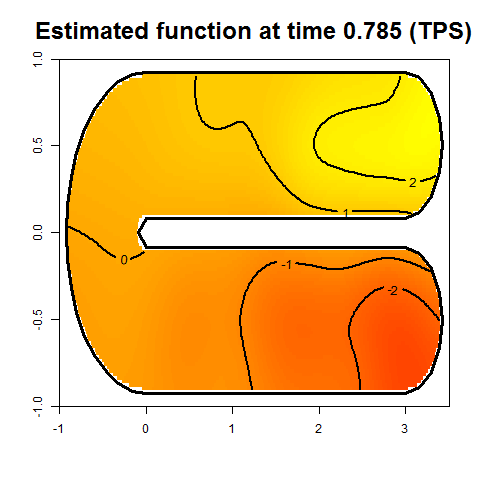
\includegraphics[trim=0cm 0cm 0cm 1.8cm,clip=true,width=0.19\textwidth,valign=t]{Immagini/simulazioni/TPStempo2.png}&
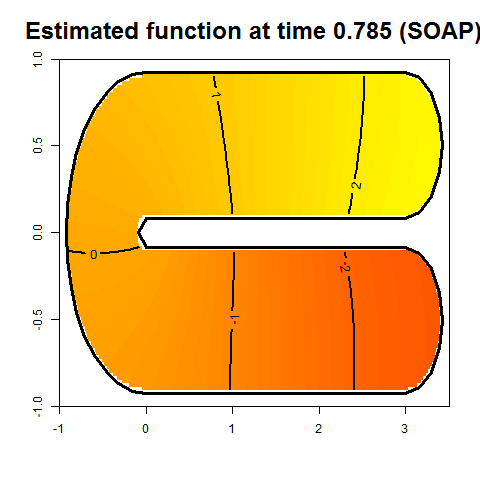
\includegraphics[trim=0cm 0cm 0cm 1.8cm,clip=true,width=0.19\textwidth,valign=t]{Immagini/simulazioni/SOAPtempo2.png}&
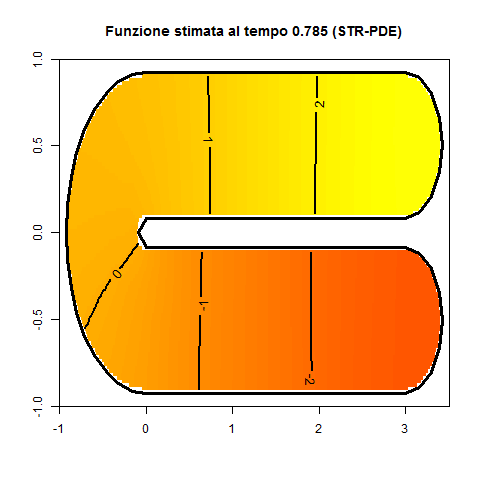
\includegraphics[trim=0cm 0cm 0cm 1.8cm,clip=true,width=0.19\textwidth,valign=t]{Immagini/simulazioni/STSRtempo2.png}\\
\parbox[t]{2mm}{\multirow{3}{*}{\rotatebox[origin=c]{90}{$t=\ 1.571$}}}&
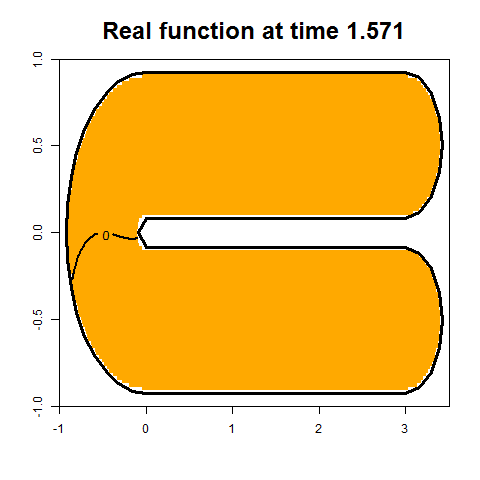
\includegraphics[trim=0cm 0cm 0cm 1.8cm,clip=true,width=0.19\textwidth,valign=t]{Immagini/simulazioni/REALEtempo3.png}&
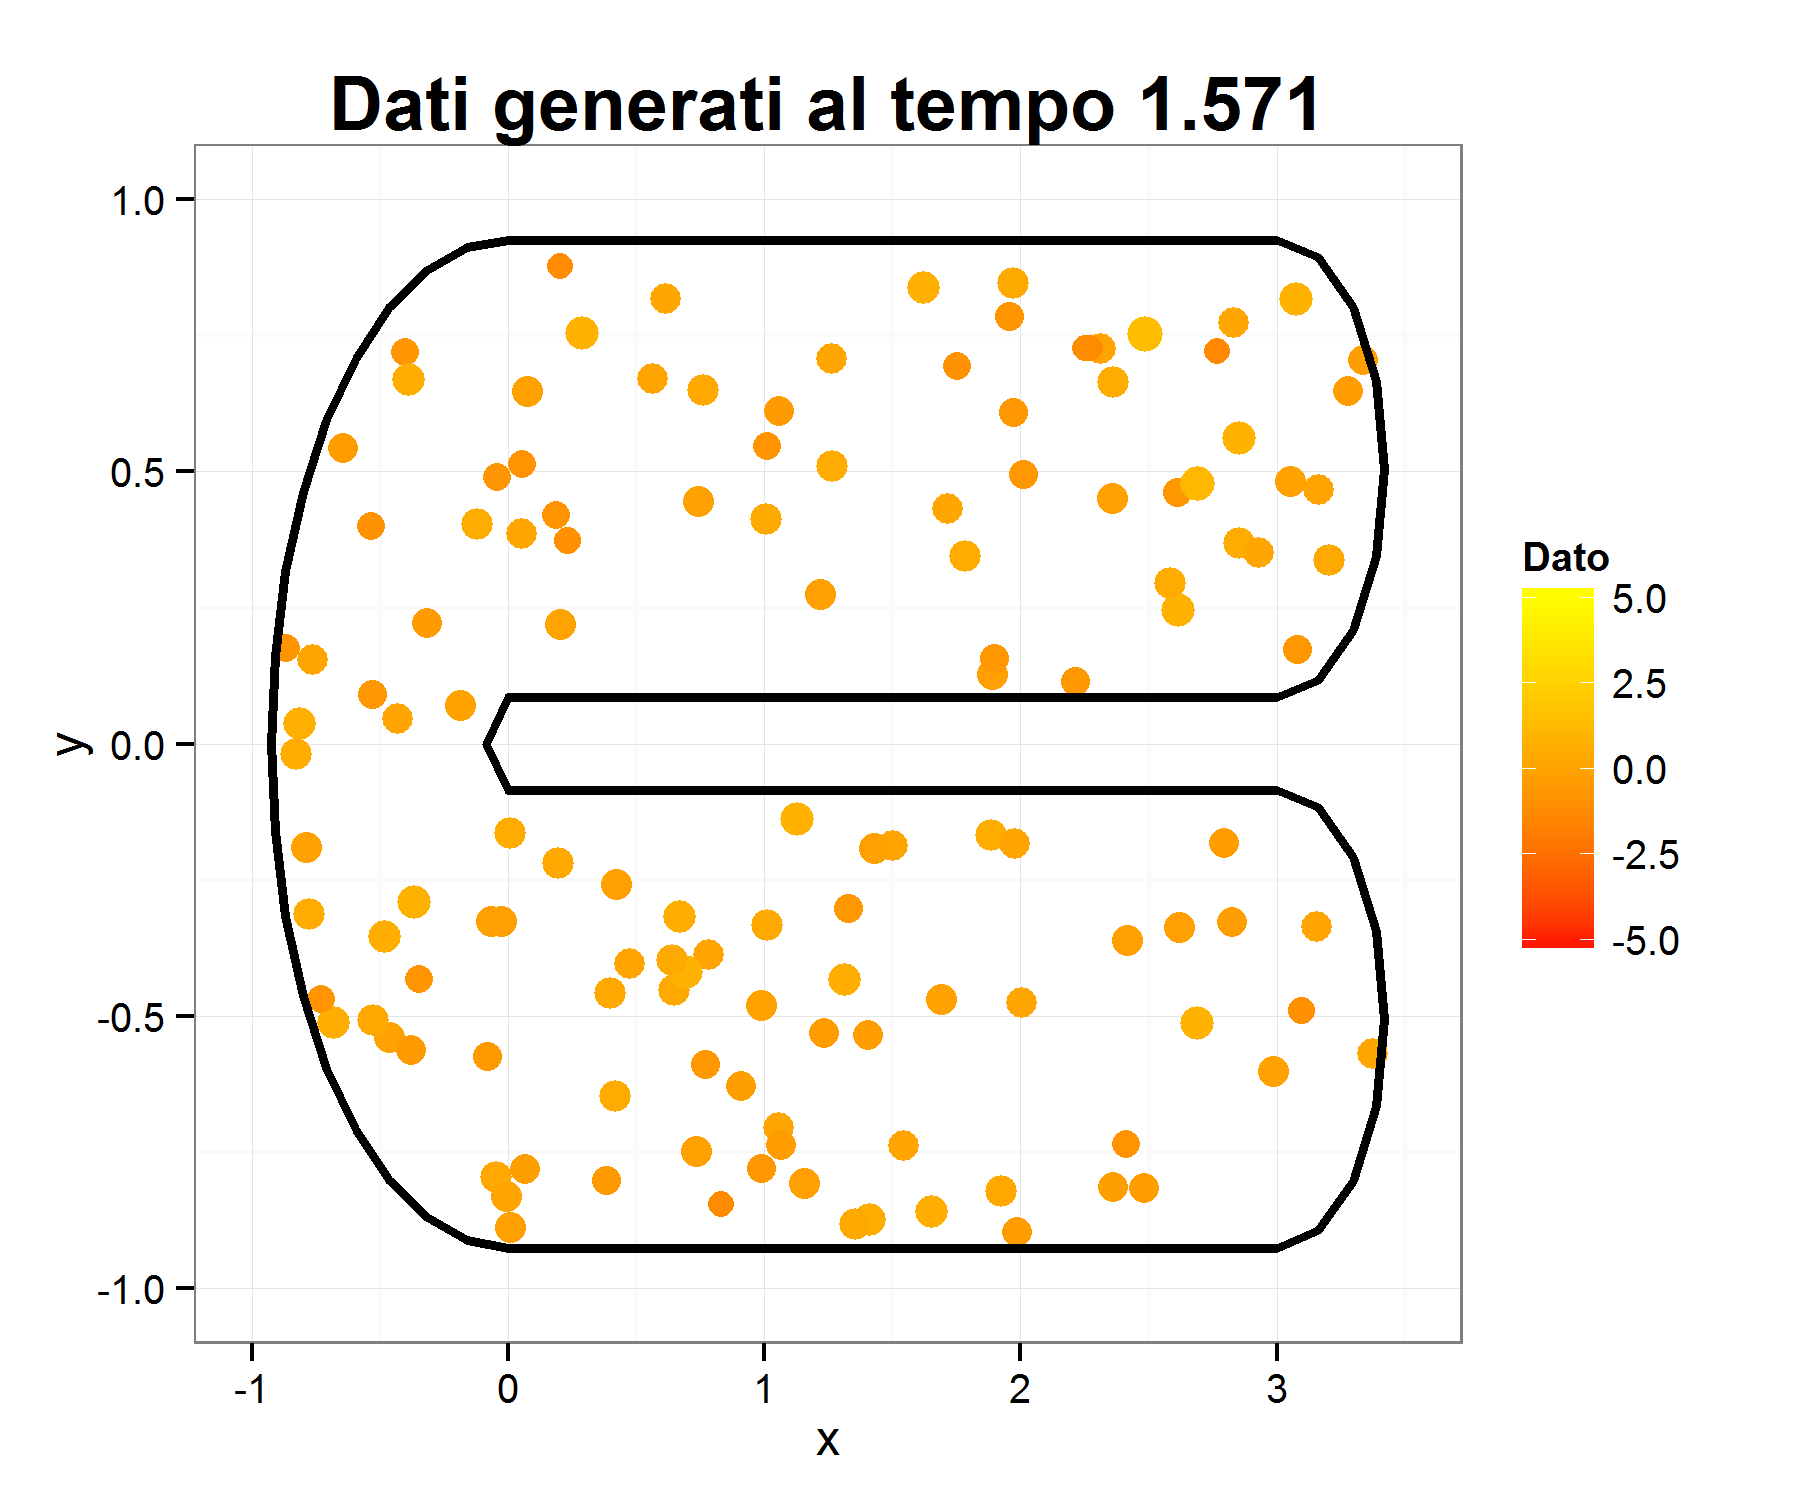
\includegraphics[trim=0.8cm 0.8cm 2.5cm 1.2cm,clip=true,width=0.19\textwidth,valign=t]{Immagini/simulazioni/Dati_tempo3.png}&
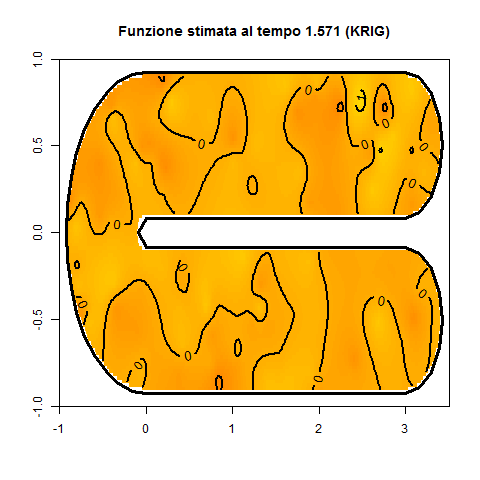
\includegraphics[trim=0cm 0cm 0cm 1.8cm,clip=true,width=0.19\textwidth,valign=t]{Immagini/simulazioni/KRIGtempo3.png}&
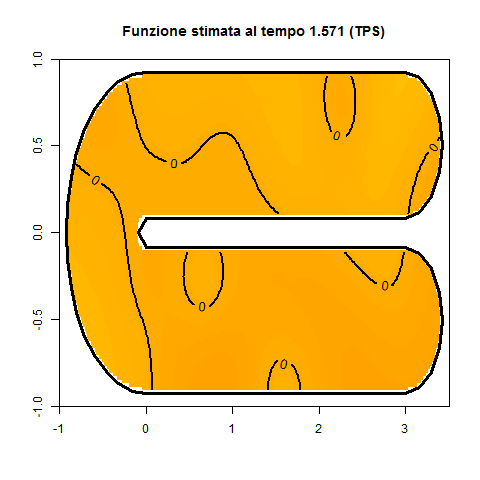
\includegraphics[trim=0cm 0cm 0cm 1.8cm,clip=true,width=0.19\textwidth,valign=t]{Immagini/simulazioni/TPStempo3.png}&
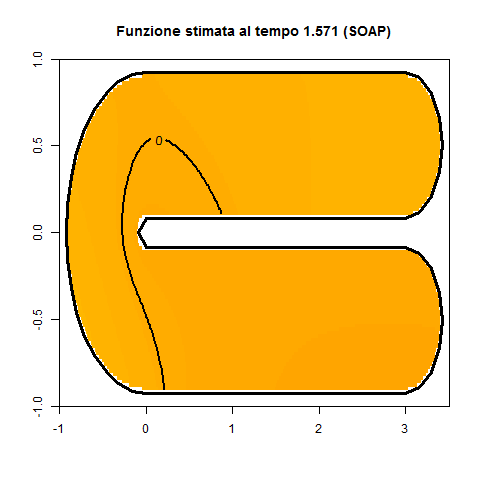
\includegraphics[trim=0cm 0cm 0cm 1.8cm,clip=true,width=0.19\textwidth,valign=t]{Immagini/simulazioni/SOAPtempo3.png}&
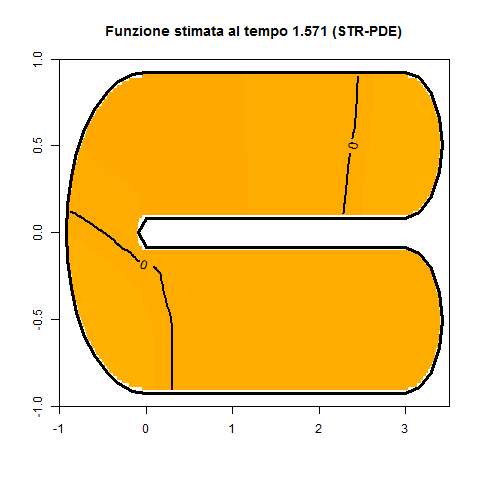
\includegraphics[trim=0cm 0cm 0cm 1.8cm,clip=true,width=0.19\textwidth,valign=t]{Immagini/simulazioni/STSRtempo3.png}\\
\parbox[t]{2mm}{\multirow{3}{*}{\rotatebox[origin=c]{90}{$t=2.356$}}}&
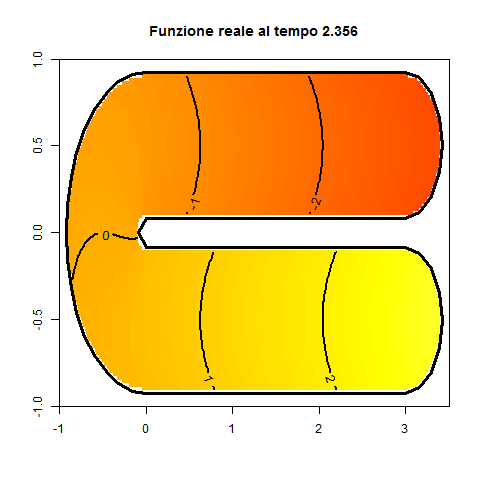
\includegraphics[trim=0cm 0cm 0cm 1.8cm,clip=true,width=0.19\textwidth,valign=t]{Immagini/simulazioni/REALEtempo4.png}&
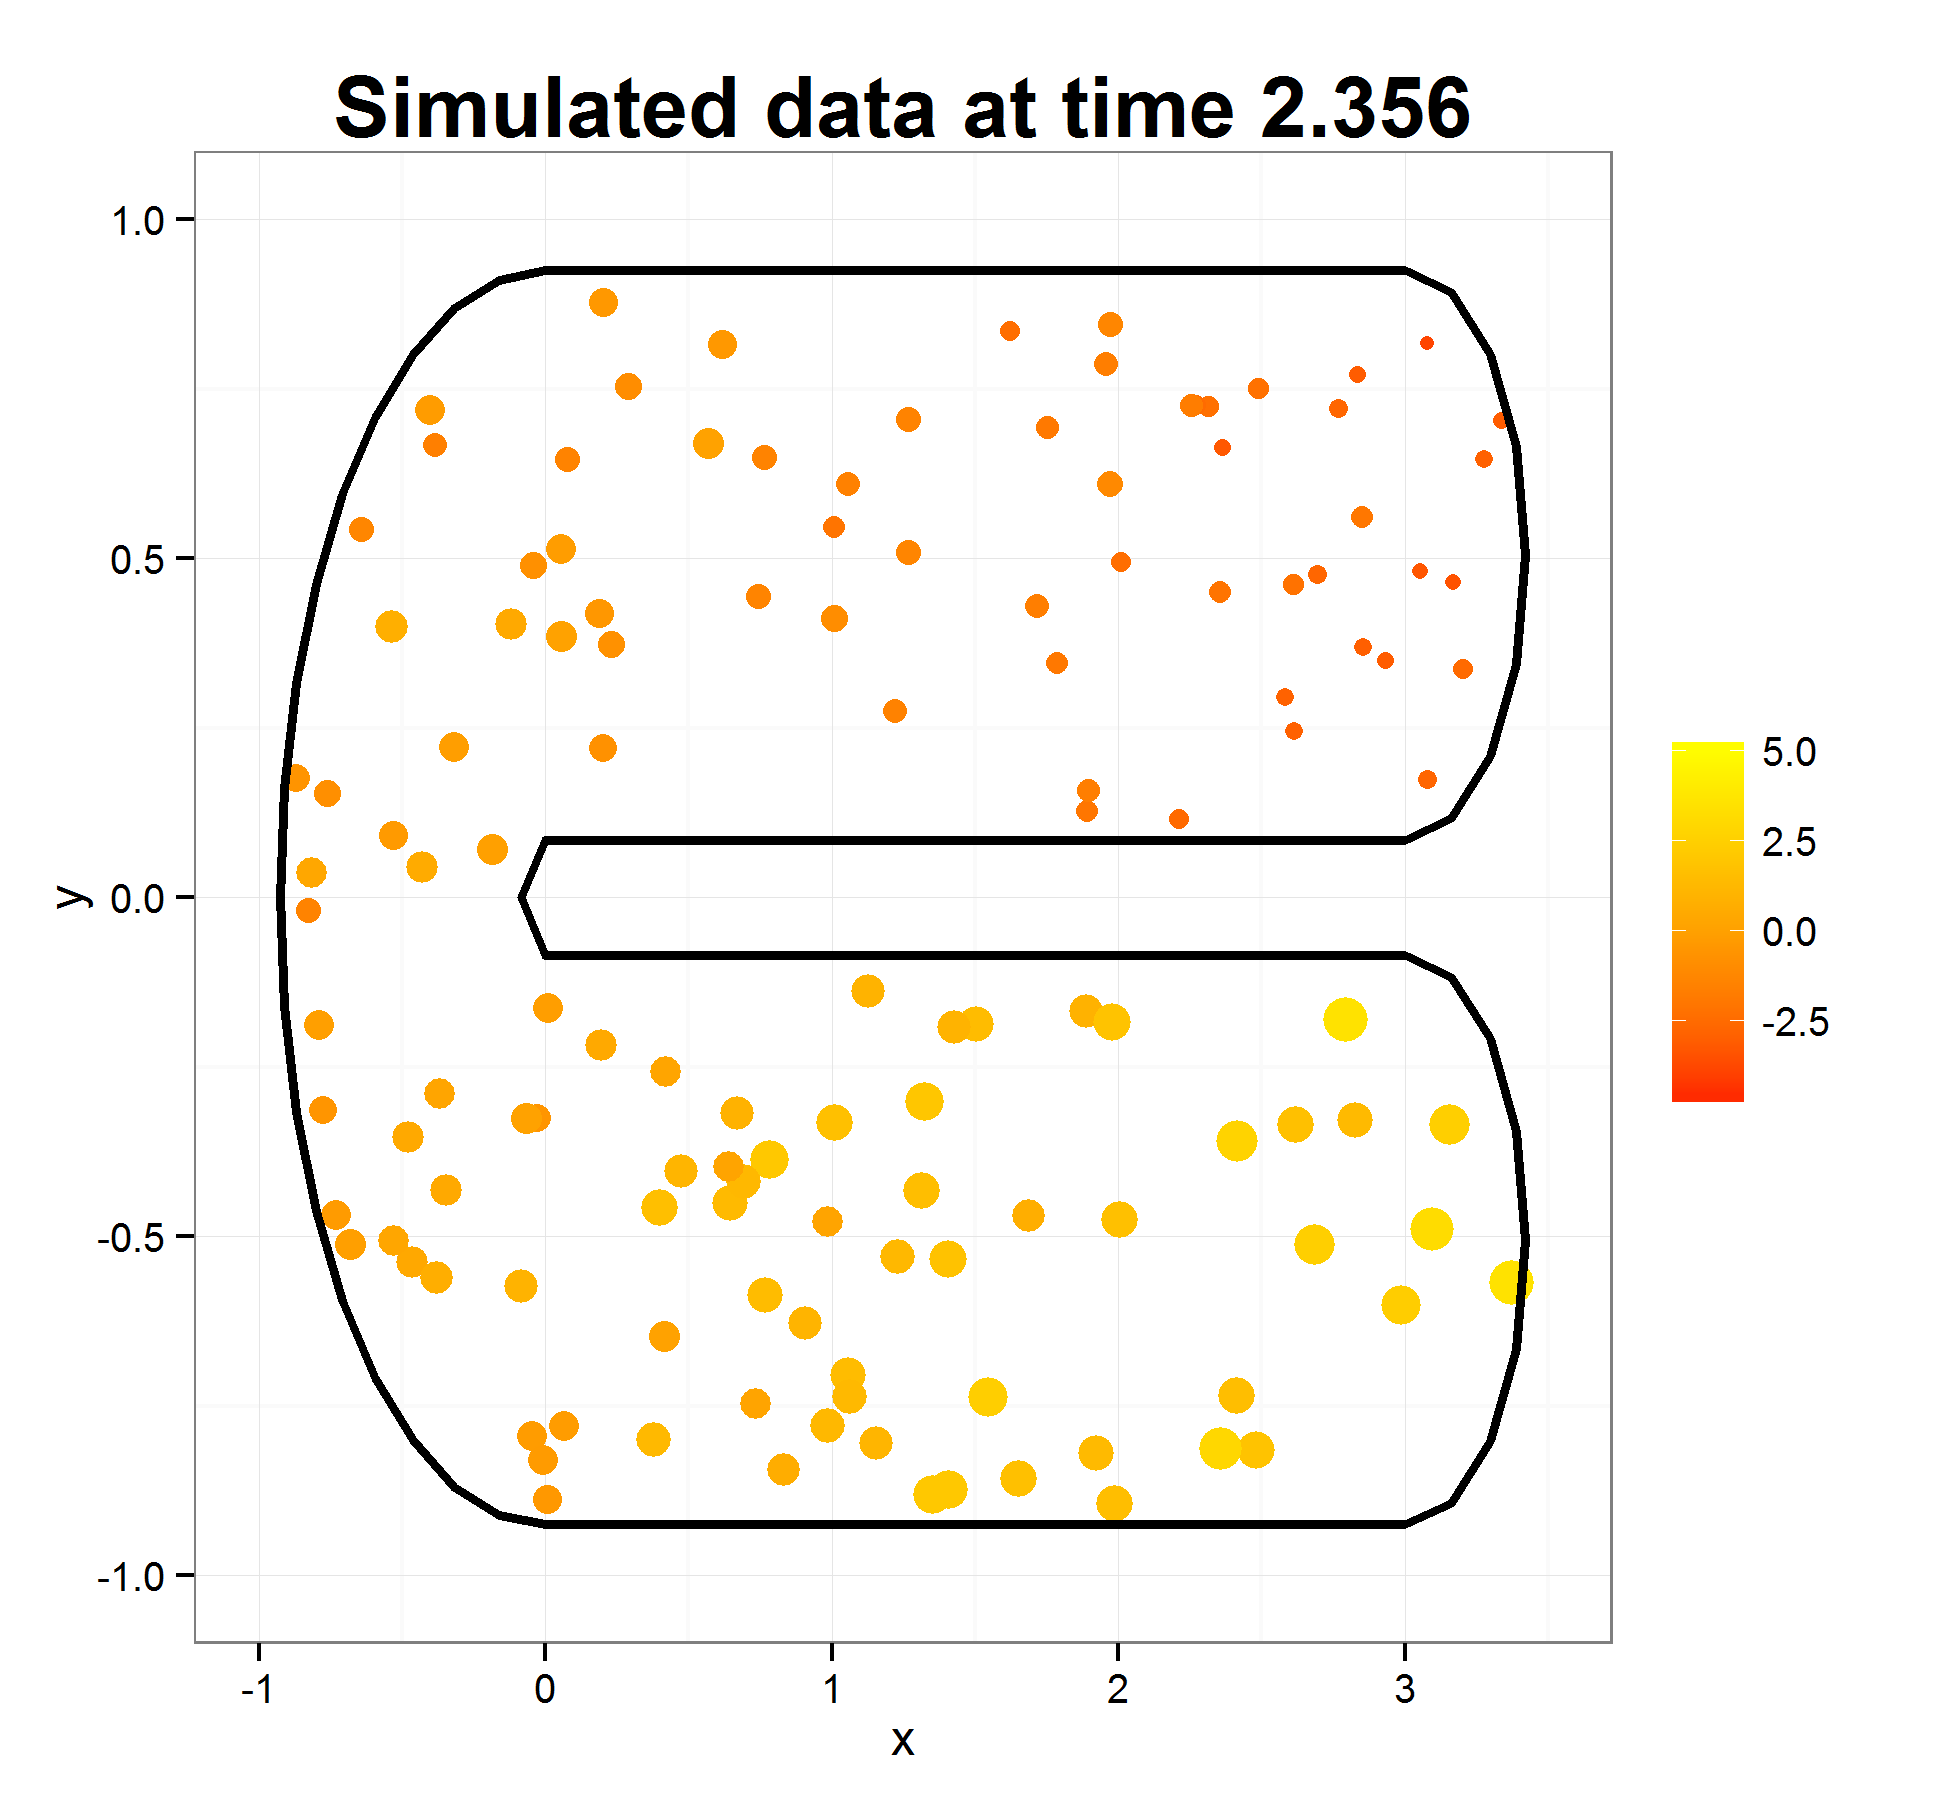
\includegraphics[trim=0.8cm 0.8cm 2.5cm 1.2cm,clip=true,width=0.19\textwidth,valign=t]{Immagini/simulazioni/Dati_tempo4.png}&
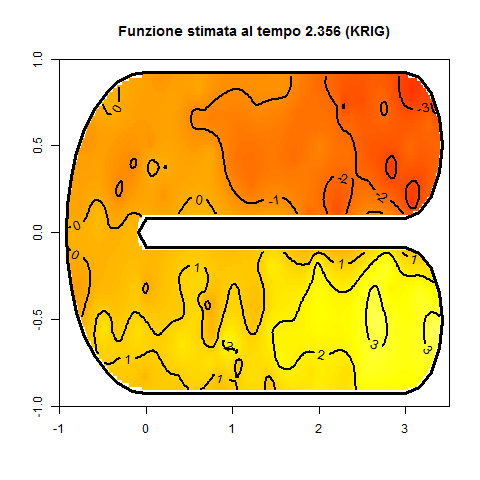
\includegraphics[trim=0cm 0cm 0cm 1.8cm,clip=true,width=0.19\textwidth,valign=t]{Immagini/simulazioni/KRIGtempo4.png}&
\includegraphics[trim=0cm 0cm 0cm 1.8cm,clip=true,width=0.19\textwidth,valign=t]{Immagini/simulazioni/TPStempo4.png}&
\includegraphics[trim=0cm 0cm 0cm 1.8cm,clip=true,width=0.19\textwidth,valign=t]{Immagini/simulazioni/SOAPtempo4.png}&
\includegraphics[trim=0cm 0cm 0cm 1.8cm,clip=true,width=0.19\textwidth,valign=t]{Immagini/simulazioni/STSRtempo4.png}

\end{tabular}
\caption{Per alcuni istanti di tempo, funzione test $f(\protect\underline{p},t)$ reale, dati simulati, stime ottenute rispettivamente con kriging spazio-temporale, soap film smoothing, thin plate splines e ST-PDE, caso senza covariata}
\label{fig:confronto_altri_metodi_nocov}
\end{figure}
\end{landscape}

\section{Caso con covariata}

La stessa analisi è stata eseguita nel caso con covariata, generata in tutti i punti esattamente come fatto nel capitolo \ref{cap:domC}. Nella calcolo del $\mathrm{RMSE}$ è stato considerato solo la parte di risposta spiegata dalla funzione $f(\underline p,t)$, poiché non è opportuno generare nuovamente valori per la covariata nei punti di validazione. I boxplot riportati in fig. \ref{fig:cfrcovar1} possono quindi essere considerati come valutazione della bontà della stima della parte funzionale del modello. Per confrontare la parte spiegata dalla covariata sono stati tracciati i boxplot in fig. \ref{fig:cfrcovar2}, con le stime di $\hat{\beta}$ calcolate durante le 50 iterazioni. Come è già stato riportato in precedenza, il kriging non è stato analizzato per alcuni problemi riguardanti l'uso del pacchetto \textit{gstat} in presenza di covariate.

Le conclusioni sono perfettamente analoghe al caso precedente. La stima di $\beta$ non presenta differenze, ma nella parte funzionale il caso ST-PDE è nuovamente il migliore. Dai plot della funzione stimata ad alcuni istanti di tempo fissati in fig. \ref{fig:confronto_altri_metodi_cov} si possono trarre le stesse conclusioni dal caso senza covariata. Il modello ST-PDE è quello che più si avvicina alla funzione reale.

\begin{figure}[t]
	\centering
	\subfigure[$\mathrm{RMSE}$]
   {
   \label{fig:cfrcovar1}
	\includegraphics[width=0.46\textwidth]{Immagini/Confronto_metodi_covar.png}   
   }
	\subfigure[Stime $\protect\hat{\beta}$]
   {
   \label{fig:cfrcovar2}
	\includegraphics[width=0.46\textwidth]{Immagini/Confronto_metodi_beta.png}
   }
	\caption{Confronto tra i metodi, caso con covariata}
	\label{fig:cfrcovar}
\end{figure}

\begin{landscape}
\begin{figure}
\centering
\begin{tabular}{lccccc}
& Funzione reale & Dati generati & TPS & SOAP & ST-PDE \\
&&&&&\\
\parbox[t]{2mm}{\multirow{3}{*}{\rotatebox[origin=r]{90}{$t=0$}}}&\includegraphics[trim=0cm 0cm 0cm 1.8cm,clip=true,width=0.19\textwidth,valign=t]{Immagini/simulazioni_covar/REALEtempo1.png} &
\includegraphics[trim=0.8cm 0.8cm 2.5cm 1.2cm,clip=true,width=0.19\textwidth,valign=t]{immagini/simulazioni_covar/Dati_tempo1.png}&
\includegraphics[trim=0cm 0cm 0cm 1.8cm,clip=true,width=0.19\textwidth,valign=t]{Immagini/simulazioni_covar/TPStempo1.png}&
\includegraphics[trim=0cm 0cm 0cm 1.8cm,clip=true,width=0.19\textwidth,valign=t]{Immagini/simulazioni_covar/SOAPtempo1.png}&
\includegraphics[trim=0cm 0cm 0cm 1.8cm,clip=true,width=0.19\textwidth,valign=t]{Immagini/simulazioni_covar/STSRtempo1.png}\\
\parbox[t]{2mm}{\multirow{3}{*}{\rotatebox[origin=c]{90}{$t=0.785$}}}&
\includegraphics[trim=0cm 0cm 0cm 1.8cm,clip=true,width=0.19\textwidth,valign=t]{Immagini/simulazioni_covar/REALEtempo2.png}&
\includegraphics[trim=0.8cm 0.8cm 2.5cm 1.2cm,clip=true,width=0.19\textwidth,valign=t]{Immagini/simulazioni_covar/Dati_tempo2.png}&
\includegraphics[trim=0cm 0cm 0cm 1.8cm,clip=true,width=0.19\textwidth,valign=t]{Immagini/simulazioni_covar/TPStempo2.png}&
\includegraphics[trim=0cm 0cm 0cm 1.8cm,clip=true,width=0.19\textwidth,valign=t]{Immagini/simulazioni_covar/SOAPtempo2.png}&
\includegraphics[trim=0cm 0cm 0cm 1.8cm,clip=true,width=0.19\textwidth,valign=t]{Immagini/simulazioni_covar/STSRtempo2.png}\\
\parbox[t]{2mm}{\multirow{3}{*}{\rotatebox[origin=c]{90}{$t=\ 1.571$}}}&
\includegraphics[trim=0cm 0cm 0cm 1.8cm,clip=true,width=0.19\textwidth,valign=t]{Immagini/simulazioni_covar/REALEtempo3.png}&
\includegraphics[trim=0.8cm 0.8cm 2.5cm 1.2cm,clip=true,width=0.19\textwidth,valign=t]{Immagini/simulazioni_covar/Dati_tempo3.png}&
\includegraphics[trim=0cm 0cm 0cm 1.8cm,clip=true,width=0.19\textwidth,valign=t]{Immagini/simulazioni_covar/TPStempo3.png}&
\includegraphics[trim=0cm 0cm 0cm 1.8cm,clip=true,width=0.19\textwidth,valign=t]{Immagini/simulazioni_covar/SOAPtempo3.png}&
\includegraphics[trim=0cm 0cm 0cm 1.8cm,clip=true,width=0.19\textwidth,valign=t]{Immagini/simulazioni_covar/STSRtempo3.png}\\
\parbox[t]{2mm}{\multirow{3}{*}{\rotatebox[origin=c]{90}{$t=2.356$}}}&
\includegraphics[trim=0cm 0cm 0cm 1.8cm,clip=true,width=0.19\textwidth,valign=t]{Immagini/simulazioni_covar/REALEtempo4.png}&
\includegraphics[trim=0.8cm 0.8cm 2.5cm 1.2cm,clip=true,width=0.19\textwidth,valign=t]{Immagini/simulazioni_covar/Dati_tempo4.png}&
\includegraphics[trim=0cm 0cm 0cm 1.8cm,clip=true,width=0.19\textwidth,valign=t]{Immagini/simulazioni_covar/TPStempo4.png}&
\includegraphics[trim=0cm 0cm 0cm 1.8cm,clip=true,width=0.19\textwidth,valign=t]{Immagini/simulazioni_covar/SOAPtempo4.png}&
\includegraphics[trim=0cm 0cm 0cm 1.8cm,clip=true,width=0.19\textwidth,valign=t]{Immagini/simulazioni_covar/STSRtempo4.png}
\end{tabular}
\caption{Per alcuni istanti di tempo, funzione test $f(\protect\underline{p},t)$ reale, dati simulati, stime ottenute rispettivamente con soap film smoothing, thin plate splines e ST-PDE, caso con covariata}
\label{fig:confronto_altri_metodi_cov}
\end{figure}
\end{landscape}


\chapter{Applicazione alla produzione di rifiuti urbani nella provincia di Venezia}
\label{cap:rifiuti}

L'applicazione principale per il modello ST-PDE in questo lavoro di tesi riguarda i dati della produzione di rifiuti urbani nel periodo di anni dal 1997 al 2011 nella provincia di Venezia. Per rifiuti urbani si intendono rifiuti domestici, rifiuti prodotti in locali, aree pubbliche, parchi, giardini o spiagge, rifiuti provenienti dalla pulizia delle strade o di altri luoghi pubblici. Non sono conteggiati i rifiuti speciali (tra cui ad esempio quelli industriali, agricoli o provenienti da attività commerciali o di costruzione) o pericolosi (per i quali esistono programmi di smaltimento particolari).

In realtà i dati raccolti dall'Agenzia Regionale per la Prevenzione e Protezione Ambientale del Veneto (Arpav) e condivisi sul sito Open Data Veneto riguardano tutta la regione. Tuttavia è stata analizzata solo la provincia di Venezia per due motivi. Innanzitutto l'interesse per la zona della laguna veneta e per le particolarità del dominio spaziale da cui essa è descritta. Inoltre considerare tutto il Veneto aumenterebbe notevolmente le dimensioni delle matrici in gioco causando una grossa spesa computazionale per la ricerca della soluzione. Quindi è stato scelto di concentrarsi su un dominio più piccolo ma nel quale è possibile notare più facilmente le caratteristiche dell'andamento del fenomeno della produzione dei rifiuti urbani e le proprietà di stima del modello.

Per ogni comune della provincia di Venezia e per ogni anno è disponibile il numero di rifiuti totali raccolti in tonnellate e la popolazione residente. La popolazione è certamente un valore influente per la produzione di rifiuti, perciò la quantità di riferimento non sarà il valore dei rifiuti totali raccolti in ogni anno per comune, ma il valore pro capite.

Le coordinate spaziali dei comuni sono la longitudine e la latitudine, disponibili on line\footnote{\href{http://www.dossier.net/utilities/coordinate-geografiche/}{http://www.dossier.net/utilities/coordinate-geografiche/}}. Nel caso dei comuni con dato replicato (sez. \ref{sez:comunireplicati}), le coordinate sono state ottenute da Google Maps.

La più importante ipotesi iniziale in questa applicazione è la scelta di riferire i dati riguardanti la raccolta dei rifiuti di tutto il territorio comunale in un unico punto, corrispondente al capoluogo. Potrebbe essere più appropriato riferire i dati all'intero territorio comunale o alla zona urbanizzata del comune (non su tutto il territorio sono prodotti rifiuti urbani). Ma per semplicità lo studio è eseguito con dati puntiformi normalizzati rispetto alla popolazione. 

\section{Il turismo come possibile covariata}

L'inclusione della popolazione residente nella risposta tramite la scelta di usare i valori pro capite è necessaria, poiché permette di depurare la risposta da una variabile che per sua natura la influenzerebbe. Ma sarebbe un errore fermarsi solo alla popolazione residente, poiché anche i turisti rappresentano una componente non trascurabile di produzione di rifiuti urbani.

Nella provincia di Venezia sono presenti molte zone di elevata attrazione turistica. Grande importanza è da attribuire a Venezia, ma si hanno anche zone balneari (come Lido di Venezia, Cavallino-Treporti, Jesolo, San Michele al Tagliamento, Bibione, ecc...). L'informazione scelta per sintetizzare l'attività turistica è il numero di posti letto totali del comune, valore disponibile grazie all'applicativo dell'Istat \textit{Atlante Statistico dei Comuni}\footnote{\href{http://www.istat.it/it/archivio/113712}{http://www.istat.it/it/archivio/113712}} per ogni anno. Il totale dei posti letto per comune è la somma di vari tipi di attività non solamente alberghiere in senso stretto (ad esempio sono conteggiati anche esercizi complementari, bed \& breakfast, campeggi) e sarà considerato normalizzato per la popolazione residente per uniformità con la risposta. I valori ricavati saranno inseriti nel modello come possibile covariata.


\section{Trattamento del dominio}

Per poter studiare il problema a livello computazionale occorre avere una buona approssimazione della frontiera della regione. Questa è disponibile nel pacchetto R \textit{raster} che descrive dati geografici di moltissime zone del mondo sia a livello nazionale che locale (nel caso italiano province e comuni) tramite poligoni molto precisi.

Una volta scaricata la provincia di Venezia da \textit{raster}, si è riscontrato subito un problema: la regione è composta da un insieme di 101 poligoni distinti (a causa delle numerose isole di cui è composta la laguna) e ogni poligono ha un alto numero di vertici (ad esempio, la prima delle due regioni corrispondenti alla parte interna della provincia ha 10538 vertici). Non è possibile analizzare il problema su un territorio così descritto, perciò è stata necessaria una analisi iniziale della frontiera per ridurne la complessità. 

\begin{figure}[t]
	\centering
	\subfigure[Tutti i poligoni]
   {
   \label{fig:Ven_poligonitutti}
	\includegraphics[width=0.46\textwidth]{Immagini/Ven_poligoni.png}   
   }
	\subfigure[Poligoni scelti]
   {
   \label{fig:Ven_poligoniscelti}
	\includegraphics[width=0.46\textwidth]{Immagini/Ven_poligoniscelti.png}
   }
	\caption{Poligoni disponibili nel pacchetto \textit{raster}}
	\label{fig:Ven_poligoni}
\end{figure}

Oltre all'entroterra (composto da due poligoni) saranno considerate solo le più più rilevanti isole della laguna a livello di popolazione e turismo: Venezia, Murano, Lido di Venezia, Pellestrina e Chioggia (composta da due poligoni). In fig. \ref{fig:Ven_poligoni} (tracciata, come per le successive, con il pacchetto R \textit{RgoogleMaps}) sono visualizzati i poligoni disponibili in \textit{raster} e quelli scelti per l'analisi. Come sarà indicato nel paragrafo successivo, tutte queste isole sono state trattate per la riduzione dei vertici e, per creare un poligono unico, sono state unite tra loro con ponti dove era possibile. Tra le isole collegate solamente via mare con il resto del territorio sono stati simulati ponti in corrispondenza delle trafficate linee di trasporto pubblico con traghetto. 

\subsection{Regression splines}

Per ridurre l'elevato numero di vertici di ognuno dei poligoni considerati (e la conseguente complessità della stima) è stato necessario ricorrere a tecniche di smoothing di dati funzionali. Ad ogni poligono è possibile associare una coppia di funzioni: la latitudine e la longitudine rispetto all'ascissa curvilinea (disponibili per punti, corrispondenti ai vertici di \textit{raster}) da rappresentare in funzioni di base. Successivamente, le nuove funzioni stimate sono state valutate in un numero molto inferiore di valori dell'ascissa curvilinea. Con le nuove coordinate ottenute dopo questo procedimento è stata costruita la nuova definizione della regione.

\begin{figure}[t]
	\centering
	\begin{minipage}{.32\textwidth}
	\includegraphics[width=\textwidth]{Immagini/Ven_Longitudine.png}
	\includegraphics[width=\textwidth]{Immagini/Ven_Latitudine.png}
	\end{minipage}%
	\begin{minipage}{.64\textwidth}
	\includegraphics[width=\textwidth]{Immagini/Ven_Regione.png}
	\end{minipage}
	\caption{Smoothing con \textit{Regression Splines} cubiche per il primo poligono dell'entroterra della provincia di Venezia}
	\label{fig:Ven_ent1}
\end{figure}

Per avere una rappresentazione ottimale tramite funzioni di base sono state provate più tecniche. La scelta definitiva è ricaduta sull'uso di \textit{Regression Splines} cubiche senza penalizzazione della derivata seconda. Infatti i risultati non sono stati migliori con le altre tecniche provate a causa della zona interna alla laguna di Venezia, fortemente frastagliata: ad esempio penalizzare la derivata seconda ha eliminato troppe asperità presenti sulle coste del territorio, mentre l'utilizzo di \textit{Kernel Smoothing} ha portato alla definizione di regioni che, dopo la triangolazione, presentavano un maggior numero di triangoli composti solamente da punti di frontiera (e quindi senza dati) rispetto agli altri metodi.

Una volta fissato un ragionevole numero di punti con cui descrivere la regione sono stati eseguiti più tentativi per decidere il miglior numero di funzioni di base. Il criterio di scelta è stato complesso, poiché sono stati esclusi i valori che generavano intersezioni nella nuova descrizione della regione e comuni esterni alla frontiera. Il miglior valore per \textit{Regression Splines} è stato quello che, una volta eseguito lo smoothing della regione, ha causato la minor distanza tra i nuovi punti della regione e il poligono iniziale di \textit{raster}. In fig. \ref{fig:Ven_ent1} è riportato il risultato dello smoothing sul primo poligono che descrive l'entroterra della provincia di Venezia (nella versione definitiva ha 100 punti, molti meno dei 10538 iniziali).  



Dopo aver ripetuto l'analisi per ognuna delle isole elencate precedentemente (eccetto Chioggia, aggregata al dominio in modo molto più semplificato), la descrizione finale è stata ricavata unendo tra loro tutti i nuovi poligoni. In seguito è stata eliminata una zona costiera dell'entroterra della laguna di Venezia che, sebbene presente sia in \textit{raster} che nei grafici di Google Maps, corrisponde ad una parte fangosa e paludosa e quindi disabitata. Non essendo possibile che su di essa siano prodotti rifiuti, è stata tagliata dalla regione. Per questo motivo si troverà sempre una zona non analizzata sui grafici con mappe di Google Maps. In fig. \ref{fig:Ven_rgm} è riportata la descrizione finale del dominio con i punti spaziali considerati.
\begin{figure}[t]
	\centering
	\subfigure[Provincia di Venezia]
   {
   \label{fig:Ven_rgm_tot}
	\includegraphics[width=0.46\textwidth]{Immagini/Ven_punti.png}   
   }
	\subfigure[Zoom della laguna]
   {
   \label{fig:Ven_rgm_zoom}
	\includegraphics[width=0.46\textwidth]{Immagini/Ven_puntizoom.png}
   }
	\caption{Frontiera e punti spaziali per la provincia di Venezia}
	\label{fig:Ven_rgm}
\end{figure}

\subsection{Replica dei dati}
\label{sez:comunireplicati}

L'uso di valori pro capite per rifiuti e posti letto consente di replicare il dato del comune anche su altri punti in cui risulta necessario. Ad esempio, le isole di Murano, Lido di Venezia e Pellestrina non sono sedi di comune, ma si riferiscono a Venezia. Quindi il dato di Venezia è stato replicato in queste isole ad ogni anno, per avere un valore di riferimento anche nelle isole. I dati replicati dal comune di Venezia sono visualizzati in rosso in fig. \ref{fig:Ven_rep1}. Come si può notare, anche nell'isola di Venezia è stato duplicato il dato, per poter ottenere una triangolazione senza troppi triangoli composti solo da punti di frontiera in una zona di particolare rilevanza. 

Un caso particolare riguarda il comune di Cavallino-Treporti, che è stato istituito nel 1999 con una parte dei territori del comune di Venezia. La separazione all'interno dei dati, però, è presente dal 2002. Di conseguenza prima di questo anno il dato in Cavallino-Treporti è una replica del dato di Venezia. Cavallino-Treporti corrisponde al punto blu in fig. \ref{fig:Ven_rep2}.

Un altro punto di replica del dato è Bibione, località balneare vicina a Lignano Sabbiadoro (che però non è in Veneto) ed interna alla regione (punto verde in fig. \ref{fig:Ven_rep2}). Il comune di riferimento di Bibione (San Michele al Tagliamento) è lontano, pertanto si genera una parte di territorio senza dati molto ampia nell'estremità orientale della provincia. Quindi la replica della misurazione in Bibione consente di avere un dato in una zona rilevante (già dai grafici in fig. \ref{fig:Ven_bubbledati} e \ref{fig:Ven_bubblePL} si potrà capire l'importanza della zona balneare in questo studio) e di coprire anche un'estremità del dominio altrimenti priva di riferimenti.

\begin{figure}[t]
\centering
\subfigure[Repliche del dato di Venezia]
   {
   \label{fig:Ven_rep1}
	\includegraphics[width=0.46\textwidth]{Immagini/Repliche1.png}   
   }
\subfigure[Cavallino-Treporti e Bibione]
   {
   \label{fig:Ven_rep2}
	\includegraphics[width=0.46\textwidth]{Immagini/Repliche2.png}
   }
\caption{Dati replicati}
\label{fig:Ven_rep}
\end{figure}


\subsection{Triangolazione del dominio}

La triangolazione è stata prodotta tramite il pacchetto R \textit{RTriangle}. Poiché nella zona ad est il numero di capoluoghi di comune (e quindi di nodi della triangolazione) è minore rispetto al resto della regione, è stata fissata un'area massima per i triangoli generati da \textit{RTriangle}. Questo ha reso la triangolazione più fitta anche dove non lo sarebbe stata, e garantirà una stima della risposta più precisa nella zona balneare che, come si potrà notare in seguito, ha una grande importanza per la distribuzione dei rifiuti. Affinchè questo sia possibile sono stati aggiunti nuovi punti spaziali all'interno della regione, che resteranno senza dato per tutta l'analisi ma saranno utili per la definizione dei triangoli. In fig. \ref{fig:Ven_triang} si ha la triangolazione finale che sarà usata da ora in avanti.

In conclusione, il dominio è descritto da 418 punti (49 con dati, 369 di frontiera o aggiunti durante la creazione della triangolazione) e da 480 triangoli.
\begin{figure}[t]
\centering
\subfigure[Provincia di Venezia]
   {
   \label{fig:Ven_triang_tot}
	\includegraphics[width=0.46\textwidth]{Immagini/Ven_triang.png}   
   }
\subfigure[Zoom della laguna]
   {
   \label{fig:Ven_triang_zoom}
	\includegraphics[width=0.46\textwidth]{Immagini/Ven_triangzoom.png}
   }
\caption{Triangolazione della provincia di Venezia}
\label{fig:Ven_triang}
\end{figure}

\section{Analisi preliminare dei dati}
Prima di eseguire l'analisi, è opportuno avere una visualizzazione dei dati sul dominio della provincia di Venezia. In fig. \ref{fig:Ven_bubbledati} e \ref{fig:Ven_bubblePL} sono visualizzati, rispettivamente, i valori dei rifiuti e dei posti letto pro capite (realizzati grazie all'aiuto del pacchetto R \textit{ggmap}), che permettono di avere un'idea della loro distribuzione in spazio e tempo.
\newpage
\begin{figure}[H]
	\centering
	\includegraphics[trim=0cm 0cm 0cm 0cm,clip=true,width=0.45\textwidth]{Immagini/venezia_dati/Dati1997.png}
	%\includegraphics[trim=0cm 0cm 0cm 2cm,clip=true,width=0.45\textwidth]{Immagini/venezia_dati/Dati1998.png}
	\includegraphics[trim=0cm 0cm 0cm 0cm,clip=true,width=0.45\textwidth]{Immagini/venezia_dati/Dati1999.png}
	%\includegraphics[trim=0cm 0cm 0cm 2cm,clip=true,width=0.45\textwidth]{Immagini/venezia_dati/Dati2000.png}
	\includegraphics[trim=0cm 0cm 0cm 0cm,clip=true,width=0.45\textwidth]{Immagini/venezia_dati/Dati2001.png}
	%\includegraphics[trim=0cm 0cm 0cm 2cm,clip=true,width=0.45\textwidth]{Immagini/venezia_dati/Dati2002.png}
	\includegraphics[trim=0cm 0cm 0cm 0cm,clip=true,width=0.45\textwidth]{Immagini/venezia_dati/Dati2003.png}
	%\includegraphics[trim=0cm 0cm 0cm 2cm,clip=true,width=0.45\textwidth]{Immagini/venezia_dati/Dati2004.png}
	\includegraphics[trim=0cm 0cm 0cm 0cm,clip=true,width=0.45\textwidth]{Immagini/venezia_dati/Dati2005.png}
	%\includegraphics[trim=0cm 0cm 0cm 2cm,clip=true,width=0.45\textwidth]{Immagini/venezia_dati/Dati2006.png}
	\includegraphics[trim=0cm 0cm 0cm 0cm,clip=true,width=0.45\textwidth]{Immagini/venezia_dati/Dati2007.png}
	%\includegraphics[trim=0cm 0cm 0cm 2cm,clip=true,width=0.45\textwidth]{Immagini/venezia_dati/Dati2008.png}
	\includegraphics[trim=0cm 0cm 0cm 0cm,clip=true,width=0.45\textwidth]{Immagini/venezia_dati/Dati2009.png}
	%\includegraphics[trim=0cm 0cm 0cm 2cm,clip=true,width=0.45\textwidth]{Immagini/venezia_dati/Dati2010.png}
	\includegraphics[trim=0cm 0cm 0cm 0cm,clip=true,width=0.45\textwidth]{Immagini/venezia_dati/Dati2011.png}
	\caption{Rifiuti urbani pro capite ogni due anni dal 1997 al 2011}
	\label{fig:Ven_bubbledati}
\end{figure}
\newpage
\begin{figure}[H]
	\centering
	\includegraphics[trim=0cm 0cm 0cm 0cm,clip=true,width=0.45\textwidth]{Immagini/venezia_dati/PL1997.png}
	%\includegraphics[trim=0cm 0cm 0cm 2cm,clip=true,width=0.45\textwidth]{Immagini/venezia_dati/PL1998.png}
	\includegraphics[trim=0cm 0cm 0cm 0cm,clip=true,width=0.45\textwidth]{Immagini/venezia_dati/PL1999.png}
	%\includegraphics[trim=0cm 0cm 0cm 2cm,clip=true,width=0.45\textwidth]{Immagini/venezia_dati/PL2000.png}
	\includegraphics[trim=0cm 0cm 0cm 0cm,clip=true,width=0.45\textwidth]{Immagini/venezia_dati/PL2001.png}
	%\includegraphics[trim=0cm 0cm 0cm 2cm,clip=true,width=0.45\textwidth]{Immagini/venezia_dati/PL2002.png}
	\includegraphics[trim=0cm 0cm 0cm 0cm,clip=true,width=0.45\textwidth]{Immagini/venezia_dati/PL2003.png}
	%\includegraphics[trim=0cm 0cm 0cm 2cm,clip=true,width=0.45\textwidth]{Immagini/venezia_dati/PL2004.png}
	\includegraphics[trim=0cm 0cm 0cm 0cm,clip=true,width=0.45\textwidth]{Immagini/venezia_dati/PL2005.png}
	%\includegraphics[trim=0cm 0cm 0cm 2cm,clip=true,width=0.45\textwidth]{Immagini/venezia_dati/PL2006.png}
	\includegraphics[trim=0cm 0cm 0cm 0cm,clip=true,width=0.45\textwidth]{Immagini/venezia_dati/PL2007.png}
	%\includegraphics[trim=0cm 0cm 0cm 2cm,clip=true,width=0.45\textwidth]{Immagini/venezia_dati/PL2008.png}
	\includegraphics[trim=0cm 0cm 0cm 0cm,clip=true,width=0.45\textwidth]{Immagini/venezia_dati/PL2009.png}
	%\includegraphics[trim=0cm 0cm 0cm 2cm,clip=true,width=0.45\textwidth]{Immagini/venezia_dati/PL2010.png}
	\includegraphics[trim=0cm 0cm 0cm 0cm,clip=true,width=0.45\textwidth]{Immagini/venezia_dati/PL2011.png}
	\caption{Posti letto pro capite ogni due anni dal 1997 al 2011}
	\label{fig:Ven_bubblePL}
\end{figure}
\newpage
\begin{figure}[t]
\centering
	\includegraphics[width=0.60\textwidth]{Immagini/Matplot.png}   
 \caption{Andamento temporale della produzione dei rifiuti urbani nei comuni}
   \label{fig:Ven_matplot}
\end{figure}
Da questa analisi iniziale si può già notare come la produzione di rifiuti sia più alta nella zona balneare della regione e come non presenti grosse variazioni nel tempo in quasi tutti i comuni, poiché i dati sono più o meno simili negli anni. Questo è evidenziato anche in fig. \ref{fig:Ven_matplot}, dove sono stati collegati tra loro i dati al variare del tempo per ogni comune. Si distinguono subito due gruppi (valori più alti per la zona balneare e più bassi negli altri comuni) totalmente distinti, eccetto per un comune (Cavallino-Treporti) che subisce un forte innalzamento nel tempo.

Dai grafici in fig. \ref{fig:Ven_bubblePL} per il numero di posti letto pro capite si può notare che la covariata assume valori decisamente più alti nella zona balneare rispetto al resto della regione. Contrariamente a quello che si potrebbe pensare, non si ha un elevato valore di posti letto nell'isola di Venezia. Invece si ha una grossa variazione nel comune di Cavallino-Treporti dopo la separazione dal comune di Venezia (si nota che il raggio della bolla aumenta notevolmente dopo il 2002). Questo indica che i posti letto sono in realtà più densi in Cavallino-Treporti, ma quando il dato era unito al comune di Venezia questo effetto non poteva essere colto in modo così dettagliato. Ci si può quindi aspettare che la funzione stimata presenti un comportamento differente in Cavallino-Treporti nelle due situazioni.

\subsection{Funzioni di base}
Le basi in spazio scelte per l'applicazione del modello sono gli elementi finiti lineari anche in questo caso. Ad ognuno dei punti spaziali (interni o di frontiera) è associata una funzione di base, coerentemente con la triangolazione prodotta. Di conseguenza si ha $N=418$ mentre il numero di punti con dati $n$ è minore ed è pari a 49.

In tempo, esattamente come nel caso del dominio a forma di C, saranno adottate come funzioni di base le B-splines cubiche. L'intervallo temporale per la descrizione del dominio è $[1997,2011]$ e i dati sono disponibili con cadenza annuale. Anche in questo caso si assume che il numero di basi sia pari al numero di istanti temporali a disposizione, quindi $M=m=15$.

\section{Applicazione del modello senza covariata}

Prima di calcolare i risultati dell'analisi occorre fissare i parametri $\lambda_S$ e $\lambda_T$. Il procedimento è perfettamente analogo a quello ricavato nel caso del dominio a forma di C per ricavare una buona approssimazione del minimo di $\mathrm{GCV}(\underline \lambda)$ in eq. \ref{eq:GCV}. A seguito di alcuni tentativi su griglie discrete, la produzione dei rifiuti è stata analizzata con $\underline \lambda = (10^{-9}, 10^{-0.125})$. In fig. \ref{fig:Ven_ris} sono riportati i risultati ottenuti nei 15 anni a disposizione. Questi grafici permettono di studiare il profilo della funzione nei vari istanti temporali in modo molto accurato, perchè la scala cromatica è stata resa uniforme tra tutti gli anni.

Successivamente sarà rappresentata anche la stima dell'evoluzione temporale della funzione in alcuni comuni, riportati in fig. \ref{fig:Ven_selected}.
\newline
\newline
\newline
\newline
\newline
\begin{figure}[h]
	\centering
	\includegraphics[width=0.45\textwidth]{Immagini/comuni_selezionati.png}   
   \caption{Comuni selezionati per l'analisi dei risultati}
	\label{fig:Ven_selected}
\end{figure}



\newpage
\begin{figure}[H]
	\centering
	\includegraphics[width=0.43\textwidth ,height=0.235\textheight]{Immagini/venezia_senza_covariate/Anno1997.png}
	\includegraphics[width=0.43\textwidth ,height=0.235\textheight]{Immagini/venezia_senza_covariate/Anno1998.png}
	\includegraphics[width=0.43\textwidth ,height=0.235\textheight]{Immagini/venezia_senza_covariate/Anno1999.png}
	\includegraphics[width=0.43\textwidth ,height=0.235\textheight]{Immagini/venezia_senza_covariate/Anno2000.png}
	\includegraphics[width=0.43\textwidth ,height=0.235\textheight]{Immagini/venezia_senza_covariate/Anno2001.png}
	\includegraphics[width=0.43\textwidth ,height=0.235\textheight]{Immagini/venezia_senza_covariate/Anno2002.png}
	\includegraphics[width=0.43\textwidth ,height=0.235\textheight]{Immagini/venezia_senza_covariate/Anno2003.png}
	\includegraphics[width=0.43\textwidth ,height=0.235\textheight]{Immagini/venezia_senza_covariate/Anno2004.png}
\end{figure}
\newpage
\begin{figure}[H]
	\centering
	\includegraphics[width=0.43\textwidth ,height=0.235\textheight]{Immagini/venezia_senza_covariate/Anno2005.png}
	\includegraphics[width=0.43\textwidth ,height=0.235\textheight]{Immagini/venezia_senza_covariate/Anno2006.png}
	\includegraphics[width=0.43\textwidth ,height=0.235\textheight]{Immagini/venezia_senza_covariate/Anno2007.png}
	\includegraphics[width=0.43\textwidth ,height=0.235\textheight]{Immagini/venezia_senza_covariate/Anno2008.png}
	\includegraphics[width=0.43\textwidth ,height=0.235\textheight]{Immagini/venezia_senza_covariate/Anno2009.png}
	\includegraphics[width=0.43\textwidth ,height=0.235\textheight]{Immagini/venezia_senza_covariate/Anno2010.png}
	\includegraphics[width=0.43\textwidth ,height=0.235\textheight]{Immagini/venezia_senza_covariate/Anno2011.png}
\caption{Stima della funzione spazio-temporale della produzione di rifiuti urbani pro capite nella provincia di Venezia a tempi fissati dal 1997 al 2011, caso senza covariata}
\label{fig:Ven_ris}
\end{figure}
\newpage

\begin{figure}[t]
	\centering
	\subfigure[Cavarzere]
   {
	\includegraphics[width=0.31\textwidth]{Immagini/venezia_senza_covariate/Cavarzere.png}   
   }
	\subfigure[Venezia]
   {
	\includegraphics[width=0.31\textwidth]{Immagini/venezia_senza_covariate/Venezia.png}
   }
	\subfigure[Cavallino-Treporti]
   {
	\includegraphics[width=0.31\textwidth]{Immagini/venezia_senza_covariate/Cavallino-Treporti.png}   
   }
	\subfigure[Jesolo]
   {
	\includegraphics[width=0.31\textwidth]{Immagini/venezia_senza_covariate/Jesolo.png}
   }
	\subfigure[Caorle]
   {
	\includegraphics[width=0.31\textwidth]{Immagini/venezia_senza_covariate/Caorle.png}   
   }
	\subfigure[Bibione]
   {
	\includegraphics[width=0.31\textwidth]{Immagini/venezia_senza_covariate/Bibione.png}
   }
	\caption{Stima della produzione di rifiuti urbani pro capite in alcuni comuni, caso senza covariata}
	\label{fig:Ven_tempo}
\end{figure}

Da tutti questi grafici è confermata la deduzione iniziale: i rifiuti sono massimi nella parte balneare della regione e minimi nella parte interna. I valori più alti si registrano in Bibione, ad est della regione. Questo conferma l'intuizione della replica del dato in questo punto. Contrariamente a quanto poteva essere supposto inizialmente, Venezia (meta turistica di fama internazionale) non è la località con la produzione più alta. Come già si notava dai grafici in fig. \ref{fig:Ven_bubblePL}, il turismo sarà rilevante nell'analisi della produzione di rifiuti e la causa non sarà Venezia (dove la produzione non è eccessivamente diversa dagli altri comuni) ma le località balneari.

Le variazioni temporali della funzione in generale non sono marcate (i grafici in fig. \ref{fig:Ven_ris} sono molto simili) ma si possono notare alcune particolarità. In fig. \ref{fig:Ven_tempo} sono tracciati gli sviluppi temporali stimati in alcuni comuni. I punti rossi corrispondono al dato misurato. La funzione stimata spiega bene l'andamento tracciato dai dati iniziali senza cadere nell'eccessiva interpolazione. Infatti, lo smoothing imposto dal modello tramite la penalizzazione della derivata seconda in tempo non permette di avere variazioni repentine poiché $\lambda_T$ non è eccessivamente basso. Ad esempio, nei grafici di Venezia e Cavallino-Treporti, i cambiamenti dovuti alla separazione del comune dal 2002 hanno provocato un mutamento dello sviluppo temporale, ma l'andamento generale è comunque colto dal modello. 

Si noti come la risposta cresca velocemente in Cavallino-Treporti (già si vedeva in fig. \ref{fig:Ven_matplot}). In fig. \ref{fig:Ven_ris} il cambiamento più marcato nel corso degli anni è proprio in questa località. La separazione dal comune di Venezia del 2002 rende il dato più preciso in Cavallino-Treporti, che successivamente cresce negli anni. Quindi l'utilizzo di questo metodo, che considera accuratamente la geometria spaziale del problema, si conferma appropriato. Se non fosse ritenuta esclusa la zona marittima della laguna, il dato di Cavallino-Treporti influenzerebbe i comuni circostanti, Venezia compresa. Invece l'effetto dell'innalzamento del dato si propaga solo verso sud-ovest, fino al termine della piccola parte di terra prima del mare.

\section{Applicazione del modello con covariata}

Le analisi sono state eseguite con $\underline \lambda = (10^{-7.625}, 10^{-0.125})$, valore ricavato come nei casi precedenti. Come si potrà notare dai prossimi grafici, dove è riportata la stima della funzione $f(\underline p,t)$ in tutti i punti senza l'aggiunta della parte spiegata dalla covariata, nelle zone dove la produzione di rifiuti pro capite era massima nel caso senza covariate ora risultano i valori più bassi.
\newpage
\begin{figure}[H]
	\centering
	\includegraphics[width=0.43\textwidth ,height=0.235\textheight]{Immagini/venezia_con_covariate/Anno1997.png}
	\includegraphics[width=0.43\textwidth ,height=0.235\textheight]{Immagini/venezia_con_covariate/Anno1998.png}
	\includegraphics[width=0.43\textwidth ,height=0.235\textheight]{Immagini/venezia_con_covariate/Anno1999.png}
	\includegraphics[width=0.43\textwidth ,height=0.235\textheight]{Immagini/venezia_con_covariate/Anno2000.png}
	\includegraphics[width=0.43\textwidth ,height=0.235\textheight]{Immagini/venezia_con_covariate/Anno2001.png}
	\includegraphics[width=0.43\textwidth ,height=0.235\textheight]{Immagini/venezia_con_covariate/Anno2002.png}
	\includegraphics[width=0.43\textwidth ,height=0.235\textheight]{Immagini/venezia_con_covariate/Anno2003.png}
	\includegraphics[width=0.43\textwidth ,height=0.235\textheight]{Immagini/venezia_con_covariate/Anno2004.png}
\end{figure}
\newpage
\begin{figure}[H]
	\centering
	\includegraphics[width=0.43\textwidth ,height=0.235\textheight]{Immagini/venezia_con_covariate/Anno2005.png}
	\includegraphics[width=0.43\textwidth ,height=0.235\textheight]{Immagini/venezia_con_covariate/Anno2006.png}
	\includegraphics[width=0.43\textwidth ,height=0.235\textheight]{Immagini/venezia_con_covariate/Anno2007.png}
	\includegraphics[width=0.43\textwidth ,height=0.235\textheight]{Immagini/venezia_con_covariate/Anno2008.png}
	\includegraphics[width=0.43\textwidth ,height=0.235\textheight]{Immagini/venezia_con_covariate/Anno2009.png}
	\includegraphics[width=0.43\textwidth ,height=0.235\textheight]{Immagini/venezia_con_covariate/Anno2010.png}
	\includegraphics[width=0.43\textwidth ,height=0.235\textheight]{Immagini/venezia_con_covariate/Anno2011.png}
\caption{Stima della parte funzionale della produzione di rifiuti urbani pro capite nella provincia di Venezia a tempi fissati dal 1997 al 2011, caso con covariata}
\label{fig:Vencovar_ris}
\end{figure}
\newpage

\begin{figure}[t]
	\centering
	\subfigure[Cavarzere]
   {
	\includegraphics[width=0.31\textwidth]{Immagini/venezia_con_covariate/Cavarzere.png}   
   }
	\subfigure[Venezia]
   {
	\includegraphics[width=0.31\textwidth]{Immagini/venezia_con_covariate/Venezia.png}
   }
	\subfigure[Cavallino-Treporti]
   {
	\includegraphics[width=0.31\textwidth]{Immagini/venezia_con_covariate/Cavallino-Treporti.png}   
   }
	\subfigure[Jesolo]
   {
	\includegraphics[width=0.31\textwidth]{Immagini/venezia_con_covariate/Jesolo.png}
   }
	\subfigure[Caorle]
   {
	\includegraphics[width=0.31\textwidth]{Immagini/venezia_con_covariate/Caorle.png}   
   }
	\subfigure[Bibione]
   {
	\includegraphics[width=0.31\textwidth]{Immagini/venezia_con_covariate/Bibione.png}
   }
	\caption{Stima della parte funzionale produzione della produzione di rifiuti urbani pro capite in alcuni comuni, caso con covariata}
	\label{fig:Vencovar_tempo}
\end{figure}
\newpage
In fig. \ref{fig:Vencovar_tempo} sono tracciati i grafici della funzione stimata (senza il termine di covariata) negli stessi comuni che sono stati scelti per il caso senza covariata. I punti tracciati in rosso rappresentano il dato senza i termine della covariata, sottratto attraverso la moltiplicazione per $\hat{\beta}$ stimato. Non possono essere considerati come la parte di dati generati esattamente dalla funzione, ma come una sua buona approssimazione (ma sono comunque ciò che è analizzato dal modello per la stime di $\hat{\underline{c}}$, come già evidenziato in sez. \ref{sez:beta}).

L'interpretazione del risultato in questo caso è legata all'alta affluenza turistica nelle zone balneari. Come già si notava dai grafici iniziali in fig. \ref{fig:Ven_bubbledati} e \ref{fig:Ven_bubblePL}, su tutta la zona costiera non si hanno solo i massimi dei rifiuti pro capite ma anche del numero di posti letto pro capite. I valori della covariata nella parte interna della regione sono quasi trascurabili rispetto alle località balneari. Quindi non solo la produzione di rifiuti è massima sulla parte settentrionale della costa, ma ancora di più, in proporzione, lo è la covariata.

Il modello stima
$$
\hat{\beta}\approx274.034 \ .
$$
Più la covariata è alta, più è sottratta informazione a $\hat{f}(\underline p,t)$ dal termine con covariata, poiché $\hat{\beta}$ è costante in spazio e tempo. Perciò la funzione ha un profilo quasi simile ad una traslazione del caso senza covariate nella parte interna del dominio (in questa zona il numero di posti letto pro capite, come era stato evidenziato in fig. \ref{fig:Ven_bubblePL}, è quasi nullo) e fortemente ribassato (talvolta fino a valori negativi) nella zona balneare a causa dell'alto contributo della covariata. Dall'intervallo di confidenza per $\beta$
$$
\beta \in [271.923;276.148]
$$
si può dedurre che la covariata non può essere esclusa dal modello.

Di nuovo è interessante il comportamento nel comune di Cavallino-Treporti, dove la funzione subisce una grossa variazione dopo la divisione dal comune di Venezia per l'aumento del numero dei posti letto. Attorno all'anno 2002 si ha un aumento molto forte della covariata (si veda fig. \ref{fig:Ven_bubblePL}), perciò la funzione si abbassa di colpo. Tuttavia, visto che questo è dovuto alla maggior precisione del dato in Cavallino-Treporti, è un cambiamento utile a spiegar meglio la risposta. Gli effetti dovuti alle proprietà di smoothing poste dal modello (non troppo interpolanti, poiché anche in questo caso $\lambda_T$ non ha un valore eccessivamente basso) portano ad un cambiamento smussato attorno all'anno della separazione del dato.
\newpage
\thispagestyle{empty}

\chapter{Conclusioni e sviluppi futuri}
\label{cap:conclusione}

In questo lavoro di tesi è stato analizzato nel dettaglio il modello ST-PDE nell'ambito della stima funzionale per dati varianti all'interno di un dominio spaziale e di un intervallo temporale. L'algoritmo di stima, particolarmente adatto a domini spaziali complessi, è stato implementato in codice R. Dal confronto con gli altri metodi e da quanto ricavato con le stime, soprattutto sul dominio a forma di C in cui è possibile conoscere il valore reale della funzione, si può concludere che i risultati prodotti sono molto buoni.

Il modello è stato proposto a seguito della necessità di dover analizzare la produzione dei rifiuti urbani tra il 1997 e il 2011 nella provincia di Venezia. I dati, disponibili per comune, sono stati localizzati in punti corrispondenti al capoluogo. Tuttavia potrebbero essere considerati in modo più preciso (ma anche più complesso) come dati areali definiti sul territorio dei comuni o sulla zona urbanizzata del comune (visto che i rifiuti urbani non sono prodotti fuori da questa zona). Quindi un possibile sviluppo futuro di questo lavoro può essere sicuramente l'estensione del modello a dati non puntiformi e la conseguente applicazione a questo problema. I risultati ottenuti dalla stima con dati puntiformi sono comunque buoni, perché spiegano appropriatamente il modello. Una conferma da un eventuale modello per dati areali, però, sarebbe senza dubbio interessante.

Diversa è la valutazione conclusiva sulle prestazioni computazionali del codice. Per semplicità le basi degli elementi finiti sono state utilizzate soltanto lineari e la produzione dei rifiuti è stata analizzata solamente nella provincia di Venezia, pur avendo a disposizione i dati di tutto il Veneto. Inoltre, durante l'esecuzione del codice, si è potuto notare come alcune funzioni come la minimizzazione di $\mathrm{GCV}(\underline \lambda)$ o il calcolo dei valori stimati ad un istante di tempo fissato (usato per tracciare il profilo della funzione ad un certo anno) siano molto lente. Ovviamente per analisi di dataset di grosse dimensioni deve essere messa in conto una spesa di tempo elevata, ma R certamente non ha aiutato. Infatti, è noto che R non sia un linguaggio di programmazione fortemente efficiente e questo ha prodotto la lentezza di esecuzione. Un chiaro sviluppo futuro può essere l'uso del codice come base per la creazione di un algoritmo più veloce attraverso l'integrazione con un linguaggio di programmazione più efficiente (come il C++) o dell'eventuale parallelizzazione nei colli di bottiglia più evidenti. Dopo che sarà stata sviluppata l'integrazione del codice sarà possibile garantire un'analisi più agile anche per dataset di dimensioni più elevate o per elementi finiti di ordine maggiore. In questo modo si avrà a disposizione uno strumento di analisi statistica buono non solo dal punto di vista dei risultati, ma anche in termini di efficienza computazionale.


\begin{thebibliography}{99}


\bibitem{art:augustin}
N.H. Augustin, V.M. Trenkel, S.N. Wood, P. Lorance, \emph{Space-time modelling of blue ling for fisheries stock management}, Environmetrics, 24, 109–119, 2013.

\bibitem{art:azzimonti}
L. Azzimonti, L.M. Sangalli, P. Secchi, M. Domanin, F. Nobile, \emph{Blood flow velocity field estimation via spatial regression with PDE penalization}, Journal of the American Statistical Association, 2015.

\bibitem{package:Matrix}
D. Bates, M. Maechler, \emph{Matrix: Sparse and Dense Matrix Classes and Methods}, R package version 1.1-5, 2015, \href{http://CRAN.R-project.org/package=Matrix}{http://CRAN.R-project.org/package=Matrix}

\bibitem{art:caballero}
W. Caballero, R. Giraldo, J. Mateu, \emph{A universal kriging approach for spatial functional data}, Stochastic Environmental Research and Risk Assessment 27(7), pp. 1553-1563, Springer, 2013.

\bibitem{art:gcv}
P. Craven, G. Wahba, \emph{Smoothing noisy data with spline functions: estimating the correct degree of smoothing by the method of generalized cross-validation}, Numerische Mathematik, 31, pp. 377–403, 1979.

\bibitem{art:cressie}
N. Cressie, C.K. Wikle, \emph{Statistics for spatio-temporal data}, John Wiley \& Sons, 2011.

\bibitem{package:raster}
R.J. Hijmans, \emph{raster: Geographic data analysis and modeling}, R package version 2.3-24, 2015. \href{http://CRAN.R-project.org/package=raster}{http://CRAN.R-project.org/package=raster}

\bibitem{package:ggmap}
D. Kahle, H. Wickham, \emph{ggmap: Spatial Visualization with ggplot2}, The R Journal, 5(1), pp. 144-161. \href{http://journal.r-project.org/archive/2013-1/kahle-wickham.pdf}{http://journal.r-project.org/archive/2013-1/kahle-wickham.pdf}

\bibitem{package:rgooglemaps}
M. Loecher, \emph{RgoogleMaps: Overlays on Google map tiles in R}, R package version 1.2.0.6, 2014. \href{http://CRAN.R-project.org/package=RgoogleMaps}{http://CRAN.R-project.org/package=RgoogleMaps}

\bibitem{art:marra}
G. Marra, D.L. Miller, Luca Zanin, \emph{Modelling the spatiotemporal distribution of the incidence of resident foreign population}, Statistica Neerlandica, 66, pp. 133–160, 2012.

\bibitem{art:menafoglio2}
A. Menafoglio, A. Guadagnini, P. Secchi, \emph{A kriging approach based on Aitchison geometry for the characterization of particle-size curves in heterogeneous aquifers}, Stochastic Environmental Research and Risk Assessment, 28(7), pp. 1835-1851, 2014.

\bibitem{art:menafoglio1}
A. Menafoglio, P. Secchi, M. Dalla Rosa et al., \emph{A Universal Kriging predictor for spatially dependent functional data of a Hilbert Space}, Electronic Journal of Statistics, 7, pp. 2209-2240, 2013.

\bibitem{package:gstat}
E.J. Pebesma, \emph{Multivariable geostatistics in S: the gstat package}, Computers \& Geosciences, 30, pp. 683-691, 2000.

\bibitem{art:quarteroni}
A. Quarteroni, \emph{Modellistica numerica per problemi differenziali}, Springer-Verlag Italia, 2012.

\bibitem{prog:R}
R Core Team, \emph{R: A Language and Environment for Statistical Computing}, R Foundation for Statistical Computing, Vienna, 2013, \href{http://www.R-project.org/}{http://www.R-project.org/}

\bibitem{art:ramsaysilverman}
J.O. Ramsay, B.W. Silverman, \emph{Functional Data Analysis}, Springer, 2005.

\bibitem{package:fda}
J.O. Ramsay, H. Wickham, S. Graves, G. Hooker, \emph{fda: Functional Data Analysis}, R package version 2.4.3, 2013, \href{http://CRAN.R-project.org/package=fda}{http://CRAN.R-project.org/package=fda}

\bibitem{art:ramsay}
T.O. Ramsay, \emph{Spline smoothing over difficult regions}, Journal of the Royal Statistical Society, Series B, 64, pp. 307–319, 2002.

\bibitem{art:sangalli}
L.M. Sangalli, J.O. Ramsay, T.O. Ramsay, \emph{Spatial spline regression models}, Journal of the Royal Statistical Society, Series B, 75, pp. 681–703, 2013.

\bibitem{package:RTriangle}
J.R. Shewchuk, \emph{Triangle: Engineering a 2D quality mesh generator and Delaunay triangulator}, in: M.C. Lin, D. Manocha (eds.), \emph{Applied Computational Geometry: Towards Geometric Engineering}, 1148, series Lecture Notes in Computer Science, pp. 203-222, Springer-Verlag, 1996. From the First ACM Workshop on Applied Computational Geometry.

\bibitem{package:ggplot2}
H. Wickham, \emph{ggplot2: elegant graphics for data analysis}, Springer New York, 2009.

\bibitem{package:mgcv1}
S.N. Wood, \emph{Fast stable restricted maximum likelihood and marginal likelihood estimation of semiparametric generalized linear models}, Journal of the Royal Statistical Society (B) 73(1), pp. 3-36, 2011.

\bibitem{package:mgcv2}
S.N. Wood, \emph{Stable and efficient multiple smoothing parameter estimation for generalized additive models}, Journal of the American Statistical Association, 99, pp. 673-686, 2004.

\bibitem{package:mgcv3}
S.N. Wood, \emph{Generalized Additive Models: An Introduction with R}, Chapman and Hall/CRC, 2006.

\bibitem{package:mgcv4}
S.N. Wood, \emph{Thin-plate regression splines}, Journal of the Royal Statistical Society (B), 65(1), pp. 95-114, 2003.
  
\bibitem{package:mgcv5}
S.N. Wood, \emph{Modelling and smoothing parameter estimation with multiple quadratic penalties}, Journal of the Royal Statistical Society (B), 62(2), pp. 413-428, 2000.

\bibitem{art:wood}
S.N. Wood, M.W. Bravington, S.L. Hedley, \emph{Soap film smoothing}, Journal of the Royal Statistical Society, Series B, 70, pp. 931–955, 2008.


\end{thebibliography}


\end{document}
